\RequirePackage{fix-cm}

\documentclass[a4paper,12pt,oneside]{book}%Minko has fleqn bonus.. I don't like: flushes equations to the left

\setlength{\textheight}{25cm}
\setlength{\textwidth}{17.5cm}
\setlength{\hoffset}{-2cm}
\setlength{\voffset}{-3cm}

\usepackage{cmap} %fixes the cyrillic search
\usepackage[utf8]{inputenc}
\usepackage[T1,T2A]{fontenc}
\usepackage[greek,bulgarian]{babel}

\usepackage{amsmath,amssymb,amsthm}

%for pseudocode obviously
\usepackage[linesnumbered,vlined,commentsnumbered,noend]{algorithm2e}

%for \definecolor
\usepackage[usenames,dvipsnames,svgnames]{xcolor}
\definecolor{AliceBlue}{rgb}{0.94,0.97,1.00}
\definecolor{AntiqueWhite1}{rgb}{1.00,0.94,0.86}
\definecolor{AntiqueWhite2}{rgb}{0.93,0.87,0.80}
\definecolor{AntiqueWhite3}{rgb}{0.80,0.75,0.69}
\definecolor{AntiqueWhite4}{rgb}{0.55,0.51,0.47}
\definecolor{AntiqueWhite}{rgb}{0.98,0.92,0.84}
\definecolor{BlanchedAlmond}{rgb}{1.00,0.92,0.80}
\definecolor{BlueViolet}{rgb}{0.54,0.17,0.89}
\definecolor{CadetBlue1}{rgb}{0.60,0.96,1.00}
\definecolor{CadetBlue2}{rgb}{0.56,0.90,0.93}
\definecolor{CadetBlue3}{rgb}{0.48,0.77,0.80}
\definecolor{CadetBlue4}{rgb}{0.33,0.53,0.55}
\definecolor{CadetBlue}{rgb}{0.37,0.62,0.63}
\definecolor{CornflowerBlue}{rgb}{0.39,0.58,0.93}
\definecolor{DarkBlue}{rgb}{0.00,0.00,0.55}
\definecolor{DarkCyan}{rgb}{0.00,0.55,0.55}
\definecolor{DarkGoldenrod1}{rgb}{1.00,0.73,0.06}
\definecolor{DarkGoldenrod2}{rgb}{0.93,0.68,0.05}
\definecolor{DarkGoldenrod3}{rgb}{0.80,0.58,0.05}
\definecolor{DarkGoldenrod4}{rgb}{0.55,0.40,0.03}
\definecolor{DarkGoldenrod}{rgb}{0.72,0.53,0.04}
\definecolor{DarkGray}{rgb}{0.66,0.66,0.66}
\definecolor{DarkGreen}{rgb}{0.00,0.39,0.00}
\definecolor{DarkGrey}{rgb}{0.66,0.66,0.66}
\definecolor{DarkKhaki}{rgb}{0.74,0.72,0.42}
\definecolor{DarkMagenta}{rgb}{0.55,0.00,0.55}
\definecolor{DarkOliveGreen1}{rgb}{0.79,1.00,0.44}
\definecolor{DarkOliveGreen2}{rgb}{0.74,0.93,0.41}
\definecolor{DarkOliveGreen3}{rgb}{0.64,0.80,0.35}
\definecolor{DarkOliveGreen4}{rgb}{0.43,0.55,0.24}
\definecolor{DarkOliveGreen}{rgb}{0.33,0.42,0.18}
\definecolor{DarkOrange1}{rgb}{1.00,0.50,0.00}
\definecolor{DarkOrange2}{rgb}{0.93,0.46,0.00}
\definecolor{DarkOrange3}{rgb}{0.80,0.40,0.00}
\definecolor{DarkOrange4}{rgb}{0.55,0.27,0.00}
\definecolor{DarkOrange}{rgb}{1.00,0.55,0.00}
\definecolor{DarkOrchid1}{rgb}{0.75,0.24,1.00}
\definecolor{DarkOrchid2}{rgb}{0.70,0.23,0.93}
\definecolor{DarkOrchid3}{rgb}{0.60,0.20,0.80}
\definecolor{DarkOrchid4}{rgb}{0.41,0.13,0.55}
\definecolor{DarkOrchid}{rgb}{0.60,0.20,0.80}
\definecolor{DarkRed}{rgb}{0.55,0.00,0.00}
\definecolor{DarkSalmon}{rgb}{0.91,0.59,0.48}
\definecolor{DarkSeaGreen1}{rgb}{0.76,1.00,0.76}
\definecolor{DarkSeaGreen2}{rgb}{0.71,0.93,0.71}
\definecolor{DarkSeaGreen3}{rgb}{0.61,0.80,0.61}
\definecolor{DarkSeaGreen4}{rgb}{0.41,0.55,0.41}
\definecolor{DarkSeaGreen}{rgb}{0.56,0.74,0.56}
\definecolor{DarkSlateBlue}{rgb}{0.28,0.24,0.55}
\definecolor{DarkSlateGray1}{rgb}{0.59,1.00,1.00}
\definecolor{DarkSlateGray2}{rgb}{0.55,0.93,0.93}
\definecolor{DarkSlateGray3}{rgb}{0.47,0.80,0.80}
\definecolor{DarkSlateGray4}{rgb}{0.32,0.55,0.55}
\definecolor{DarkSlateGray}{rgb}{0.18,0.31,0.31}
\definecolor{DarkSlateGrey}{rgb}{0.18,0.31,0.31}
\definecolor{DarkTurquoise}{rgb}{0.00,0.81,0.82}
\definecolor{DarkViolet}{rgb}{0.58,0.00,0.83}
\definecolor{DeepPink1}{rgb}{1.00,0.08,0.58}
\definecolor{DeepPink2}{rgb}{0.93,0.07,0.54}
\definecolor{DeepPink3}{rgb}{0.80,0.06,0.46}
\definecolor{DeepPink4}{rgb}{0.55,0.04,0.31}
\definecolor{DeepPink}{rgb}{1.00,0.08,0.58}
\definecolor{DeepSkyBlue1}{rgb}{0.00,0.75,1.00}
\definecolor{DeepSkyBlue2}{rgb}{0.00,0.70,0.93}
\definecolor{DeepSkyBlue3}{rgb}{0.00,0.60,0.80}
\definecolor{DeepSkyBlue4}{rgb}{0.00,0.41,0.55}
\definecolor{DeepSkyBlue}{rgb}{0.00,0.75,1.00}
\definecolor{DimGray}{rgb}{0.41,0.41,0.41}
\definecolor{DimGrey}{rgb}{0.41,0.41,0.41}
\definecolor{DodgerBlue1}{rgb}{0.12,0.56,1.00}
\definecolor{DodgerBlue2}{rgb}{0.11,0.53,0.93}
\definecolor{DodgerBlue3}{rgb}{0.09,0.45,0.80}
\definecolor{DodgerBlue4}{rgb}{0.06,0.31,0.55}
\definecolor{DodgerBlue}{rgb}{0.12,0.56,1.00}
\definecolor{FloralWhite}{rgb}{1.00,0.98,0.94}
\definecolor{ForestGreen}{rgb}{0.13,0.55,0.13}
\definecolor{GhostWhite}{rgb}{0.97,0.97,1.00}
\definecolor{GreenYellow}{rgb}{0.68,1.00,0.18}
\definecolor{HotPink1}{rgb}{1.00,0.43,0.71}
\definecolor{HotPink2}{rgb}{0.93,0.42,0.65}
\definecolor{HotPink3}{rgb}{0.80,0.38,0.56}
\definecolor{HotPink4}{rgb}{0.55,0.23,0.38}
\definecolor{HotPink}{rgb}{1.00,0.41,0.71}
\definecolor{IndianRed1}{rgb}{1.00,0.42,0.42}
\definecolor{IndianRed2}{rgb}{0.93,0.39,0.39}
\definecolor{IndianRed3}{rgb}{0.80,0.33,0.33}
\definecolor{IndianRed4}{rgb}{0.55,0.23,0.23}
\definecolor{IndianRed}{rgb}{0.80,0.36,0.36}
\definecolor{LavenderBlush1}{rgb}{1.00,0.94,0.96}
\definecolor{LavenderBlush2}{rgb}{0.93,0.88,0.90}
\definecolor{LavenderBlush3}{rgb}{0.80,0.76,0.77}
\definecolor{LavenderBlush4}{rgb}{0.55,0.51,0.53}
\definecolor{LavenderBlush}{rgb}{1.00,0.94,0.96}
\definecolor{LawnGreen}{rgb}{0.49,0.99,0.00}
\definecolor{LemonChiffon1}{rgb}{1.00,0.98,0.80}
\definecolor{LemonChiffon2}{rgb}{0.93,0.91,0.75}
\definecolor{LemonChiffon3}{rgb}{0.80,0.79,0.65}
\definecolor{LemonChiffon4}{rgb}{0.55,0.54,0.44}
\definecolor{LemonChiffon}{rgb}{1.00,0.98,0.80}
\definecolor{LightBlue1}{rgb}{0.75,0.94,1.00}
\definecolor{LightBlue2}{rgb}{0.70,0.87,0.93}
\definecolor{LightBlue3}{rgb}{0.60,0.75,0.80}
\definecolor{LightBlue4}{rgb}{0.41,0.51,0.55}
\definecolor{LightBlue}{rgb}{0.68,0.85,0.90}
\definecolor{LightCoral}{rgb}{0.94,0.50,0.50}
\definecolor{LightCyan1}{rgb}{0.88,1.00,1.00}
\definecolor{LightCyan2}{rgb}{0.82,0.93,0.93}
\definecolor{LightCyan3}{rgb}{0.71,0.80,0.80}
\definecolor{LightCyan4}{rgb}{0.48,0.55,0.55}
\definecolor{LightCyan}{rgb}{0.88,1.00,1.00}
\definecolor{LightGoldenrod1}{rgb}{1.00,0.93,0.55}
\definecolor{LightGoldenrod2}{rgb}{0.93,0.86,0.51}
\definecolor{LightGoldenrod3}{rgb}{0.80,0.75,0.44}
\definecolor{LightGoldenrod4}{rgb}{0.55,0.51,0.30}
\definecolor{LightGoldenrodYellow}{rgb}{0.98,0.98,0.82}
\definecolor{LightGoldenrod}{rgb}{0.93,0.87,0.51}
\definecolor{LightGray}{rgb}{0.83,0.83,0.83}
\definecolor{LightGreen}{rgb}{0.56,0.93,0.56}
\definecolor{LightGrey}{rgb}{0.83,0.83,0.83}
\definecolor{LightPink1}{rgb}{1.00,0.68,0.73}
\definecolor{LightPink2}{rgb}{0.93,0.64,0.68}
\definecolor{LightPink3}{rgb}{0.80,0.55,0.58}
\definecolor{LightPink4}{rgb}{0.55,0.37,0.40}
\definecolor{LightPink}{rgb}{1.00,0.71,0.76}
\definecolor{LightSalmon1}{rgb}{1.00,0.63,0.48}
\definecolor{LightSalmon2}{rgb}{0.93,0.58,0.45}
\definecolor{LightSalmon3}{rgb}{0.80,0.51,0.38}
\definecolor{LightSalmon4}{rgb}{0.55,0.34,0.26}
\definecolor{LightSalmon}{rgb}{1.00,0.63,0.48}
\definecolor{LightSeaGreen}{rgb}{0.13,0.70,0.67}
\definecolor{LightSkyBlue1}{rgb}{0.69,0.89,1.00}
\definecolor{LightSkyBlue2}{rgb}{0.64,0.83,0.93}
\definecolor{LightSkyBlue3}{rgb}{0.55,0.71,0.80}
\definecolor{LightSkyBlue4}{rgb}{0.38,0.48,0.55}
\definecolor{LightSkyBlue}{rgb}{0.53,0.81,0.98}
\definecolor{LightSlateBlue}{rgb}{0.52,0.44,1.00}
\definecolor{LightSlateGray}{rgb}{0.47,0.53,0.60}
\definecolor{LightSlateGrey}{rgb}{0.47,0.53,0.60}
\definecolor{LightSteelBlue1}{rgb}{0.79,0.88,1.00}
\definecolor{LightSteelBlue2}{rgb}{0.74,0.82,0.93}
\definecolor{LightSteelBlue3}{rgb}{0.64,0.71,0.80}
\definecolor{LightSteelBlue4}{rgb}{0.43,0.48,0.55}
\definecolor{LightSteelBlue}{rgb}{0.69,0.77,0.87}
\definecolor{LightYellow1}{rgb}{1.00,1.00,0.88}
\definecolor{LightYellow2}{rgb}{0.93,0.93,0.82}
\definecolor{LightYellow3}{rgb}{0.80,0.80,0.71}
\definecolor{LightYellow4}{rgb}{0.55,0.55,0.48}
\definecolor{LightYellow}{rgb}{1.00,1.00,0.88}
\definecolor{LimeGreen}{rgb}{0.20,0.80,0.20}
\definecolor{MediumAquamarine}{rgb}{0.40,0.80,0.67}
\definecolor{MediumBlue}{rgb}{0.00,0.00,0.80}
\definecolor{MediumOrchid1}{rgb}{0.88,0.40,1.00}
\definecolor{MediumOrchid2}{rgb}{0.82,0.37,0.93}
\definecolor{MediumOrchid3}{rgb}{0.71,0.32,0.80}
\definecolor{MediumOrchid4}{rgb}{0.48,0.22,0.55}
\definecolor{MediumOrchid}{rgb}{0.73,0.33,0.83}
\definecolor{MediumPurple1}{rgb}{0.67,0.51,1.00}
\definecolor{MediumPurple2}{rgb}{0.62,0.47,0.93}
\definecolor{MediumPurple3}{rgb}{0.54,0.41,0.80}
\definecolor{MediumPurple4}{rgb}{0.36,0.28,0.55}
\definecolor{MediumPurple}{rgb}{0.58,0.44,0.86}
\definecolor{MediumSeaGreen}{rgb}{0.24,0.70,0.44}
\definecolor{MediumSlateBlue}{rgb}{0.48,0.41,0.93}
\definecolor{MediumSpringGreen}{rgb}{0.00,0.98,0.60}
\definecolor{MediumTurquoise}{rgb}{0.28,0.82,0.80}
\definecolor{MediumVioletRed}{rgb}{0.78,0.08,0.52}
\definecolor{MidnightBlue}{rgb}{0.10,0.10,0.44}
\definecolor{MintCream}{rgb}{0.96,1.00,0.98}
\definecolor{MistyRose1}{rgb}{1.00,0.89,0.88}
\definecolor{MistyRose2}{rgb}{0.93,0.84,0.82}
\definecolor{MistyRose3}{rgb}{0.80,0.72,0.71}
\definecolor{MistyRose4}{rgb}{0.55,0.49,0.48}
\definecolor{MistyRose}{rgb}{1.00,0.89,0.88}
\definecolor{NavajoWhite1}{rgb}{1.00,0.87,0.68}
\definecolor{NavajoWhite2}{rgb}{0.93,0.81,0.63}
\definecolor{NavajoWhite3}{rgb}{0.80,0.70,0.55}
\definecolor{NavajoWhite4}{rgb}{0.55,0.47,0.37}
\definecolor{NavajoWhite}{rgb}{1.00,0.87,0.68}
\definecolor{NavyBlue}{rgb}{0.00,0.00,0.50}
\definecolor{OldLace}{rgb}{0.99,0.96,0.90}
\definecolor{OliveDrab1}{rgb}{0.75,1.00,0.24}
\definecolor{OliveDrab2}{rgb}{0.70,0.93,0.23}
\definecolor{OliveDrab3}{rgb}{0.60,0.80,0.20}
\definecolor{OliveDrab4}{rgb}{0.41,0.55,0.13}
\definecolor{OliveDrab}{rgb}{0.42,0.56,0.14}
\definecolor{OrangeRed1}{rgb}{1.00,0.27,0.00}
\definecolor{OrangeRed2}{rgb}{0.93,0.25,0.00}
\definecolor{OrangeRed3}{rgb}{0.80,0.22,0.00}
\definecolor{OrangeRed4}{rgb}{0.55,0.15,0.00}
\definecolor{OrangeRed}{rgb}{1.00,0.27,0.00}
\definecolor{PaleGoldenrod}{rgb}{0.93,0.91,0.67}
\definecolor{PaleGreen1}{rgb}{0.60,1.00,0.60}
\definecolor{PaleGreen2}{rgb}{0.56,0.93,0.56}
\definecolor{PaleGreen3}{rgb}{0.49,0.80,0.49}
\definecolor{PaleGreen4}{rgb}{0.33,0.55,0.33}
\definecolor{PaleGreen}{rgb}{0.60,0.98,0.60}
\definecolor{PaleTurquoise1}{rgb}{0.73,1.00,1.00}
\definecolor{PaleTurquoise2}{rgb}{0.68,0.93,0.93}
\definecolor{PaleTurquoise3}{rgb}{0.59,0.80,0.80}
\definecolor{PaleTurquoise4}{rgb}{0.40,0.55,0.55}
\definecolor{PaleTurquoise}{rgb}{0.69,0.93,0.93}
\definecolor{PaleVioletRed1}{rgb}{1.00,0.51,0.67}
\definecolor{PaleVioletRed2}{rgb}{0.93,0.47,0.62}
\definecolor{PaleVioletRed3}{rgb}{0.80,0.41,0.54}
\definecolor{PaleVioletRed4}{rgb}{0.55,0.28,0.36}
\definecolor{PaleVioletRed}{rgb}{0.86,0.44,0.58}
\definecolor{PapayaWhip}{rgb}{1.00,0.94,0.84}
\definecolor{PeachPuff1}{rgb}{1.00,0.85,0.73}
\definecolor{PeachPuff2}{rgb}{0.93,0.80,0.68}
\definecolor{PeachPuff3}{rgb}{0.80,0.69,0.58}
\definecolor{PeachPuff4}{rgb}{0.55,0.47,0.40}
\definecolor{PeachPuff}{rgb}{1.00,0.85,0.73}
\definecolor{PowderBlue}{rgb}{0.69,0.88,0.90}
\definecolor{RosyBrown1}{rgb}{1.00,0.76,0.76}
\definecolor{RosyBrown2}{rgb}{0.93,0.71,0.71}
\definecolor{RosyBrown3}{rgb}{0.80,0.61,0.61}
\definecolor{RosyBrown4}{rgb}{0.55,0.41,0.41}
\definecolor{RosyBrown}{rgb}{0.74,0.56,0.56}
\definecolor{RoyalBlue1}{rgb}{0.28,0.46,1.00}
\definecolor{RoyalBlue2}{rgb}{0.26,0.43,0.93}
\definecolor{RoyalBlue3}{rgb}{0.23,0.37,0.80}
\definecolor{RoyalBlue4}{rgb}{0.15,0.25,0.55}
\definecolor{RoyalBlue}{rgb}{0.25,0.41,0.88}
\definecolor{SaddleBrown}{rgb}{0.55,0.27,0.07}
\definecolor{SandyBrown}{rgb}{0.96,0.64,0.38}
\definecolor{SeaGreen1}{rgb}{0.33,1.00,0.62}
\definecolor{SeaGreen2}{rgb}{0.31,0.93,0.58}
\definecolor{SeaGreen3}{rgb}{0.26,0.80,0.50}
\definecolor{SeaGreen4}{rgb}{0.18,0.55,0.34}
\definecolor{SeaGreen}{rgb}{0.18,0.55,0.34}
\definecolor{SkyBlue1}{rgb}{0.53,0.81,1.00}
\definecolor{SkyBlue2}{rgb}{0.49,0.75,0.93}
\definecolor{SkyBlue3}{rgb}{0.42,0.65,0.80}
\definecolor{SkyBlue4}{rgb}{0.29,0.44,0.55}
\definecolor{SkyBlue}{rgb}{0.53,0.81,0.92}
\definecolor{SlateBlue1}{rgb}{0.51,0.44,1.00}
\definecolor{SlateBlue2}{rgb}{0.48,0.40,0.93}
\definecolor{SlateBlue3}{rgb}{0.41,0.35,0.80}
\definecolor{SlateBlue4}{rgb}{0.28,0.24,0.55}
\definecolor{SlateBlue}{rgb}{0.42,0.35,0.80}
\definecolor{SlateGray1}{rgb}{0.78,0.89,1.00}
\definecolor{SlateGray2}{rgb}{0.73,0.83,0.93}
\definecolor{SlateGray3}{rgb}{0.62,0.71,0.80}
\definecolor{SlateGray4}{rgb}{0.42,0.48,0.55}
\definecolor{SlateGray}{rgb}{0.44,0.50,0.56}
\definecolor{SlateGrey}{rgb}{0.44,0.50,0.56}
\definecolor{SpringGreen1}{rgb}{0.00,1.00,0.50}
\definecolor{SpringGreen2}{rgb}{0.00,0.93,0.46}
\definecolor{SpringGreen3}{rgb}{0.00,0.80,0.40}
\definecolor{SpringGreen4}{rgb}{0.00,0.55,0.27}
\definecolor{SpringGreen}{rgb}{0.00,1.00,0.50}
\definecolor{SteelBlue1}{rgb}{0.39,0.72,1.00}
\definecolor{SteelBlue2}{rgb}{0.36,0.67,0.93}
\definecolor{SteelBlue3}{rgb}{0.31,0.58,0.80}
\definecolor{SteelBlue4}{rgb}{0.21,0.39,0.55}
\definecolor{SteelBlue}{rgb}{0.27,0.51,0.71}
\definecolor{VioletRed1}{rgb}{1.00,0.24,0.59}
\definecolor{VioletRed2}{rgb}{0.93,0.23,0.55}
\definecolor{VioletRed3}{rgb}{0.80,0.20,0.47}
\definecolor{VioletRed4}{rgb}{0.55,0.13,0.32}
\definecolor{VioletRed}{rgb}{0.82,0.13,0.56}
\definecolor{WhiteSmoke}{rgb}{0.96,0.96,0.96}
\definecolor{YellowGreen}{rgb}{0.60,0.80,0.20}
\definecolor{aliceblue}{rgb}{0.94,0.97,1.00}
\definecolor{antiquewhite}{rgb}{0.98,0.92,0.84}
\definecolor{aquamarine1}{rgb}{0.50,1.00,0.83}
\definecolor{aquamarine2}{rgb}{0.46,0.93,0.78}
\definecolor{aquamarine3}{rgb}{0.40,0.80,0.67}
\definecolor{aquamarine4}{rgb}{0.27,0.55,0.45}
\definecolor{aquamarine}{rgb}{0.50,1.00,0.83}
\definecolor{azure1}{rgb}{0.94,1.00,1.00}
\definecolor{azure2}{rgb}{0.88,0.93,0.93}
\definecolor{azure3}{rgb}{0.76,0.80,0.80}
\definecolor{azure4}{rgb}{0.51,0.55,0.55}
\definecolor{azure}{rgb}{0.94,1.00,1.00}
\definecolor{beige}{rgb}{0.96,0.96,0.86}
\definecolor{bisque1}{rgb}{1.00,0.89,0.77}
\definecolor{bisque2}{rgb}{0.93,0.84,0.72}
\definecolor{bisque3}{rgb}{0.80,0.72,0.62}
\definecolor{bisque4}{rgb}{0.55,0.49,0.42}
\definecolor{bisque}{rgb}{1.00,0.89,0.77}
\definecolor{black}{rgb}{0.00,0.00,0.00}
\definecolor{blanchedalmond}{rgb}{1.00,0.92,0.80}
\definecolor{blue1}{rgb}{0.00,0.00,1.00}
\definecolor{blue2}{rgb}{0.00,0.00,0.93}
\definecolor{blue3}{rgb}{0.00,0.00,0.80}
\definecolor{blue4}{rgb}{0.00,0.00,0.55}
\definecolor{blueviolet}{rgb}{0.54,0.17,0.89}
\definecolor{blue}{rgb}{0.00,0.00,1.00}
\definecolor{brown1}{rgb}{1.00,0.25,0.25}
\definecolor{brown2}{rgb}{0.93,0.23,0.23}
\definecolor{brown3}{rgb}{0.80,0.20,0.20}
\definecolor{brown4}{rgb}{0.55,0.14,0.14}
\definecolor{brown}{rgb}{0.65,0.16,0.16}
\definecolor{burlywood1}{rgb}{1.00,0.83,0.61}
\definecolor{burlywood2}{rgb}{0.93,0.77,0.57}
\definecolor{burlywood3}{rgb}{0.80,0.67,0.49}
\definecolor{burlywood4}{rgb}{0.55,0.45,0.33}
\definecolor{burlywood}{rgb}{0.87,0.72,0.53}
\definecolor{cadetblue}{rgb}{0.37,0.62,0.63}
\definecolor{chartreuse1}{rgb}{0.50,1.00,0.00}
\definecolor{chartreuse2}{rgb}{0.46,0.93,0.00}
\definecolor{chartreuse3}{rgb}{0.40,0.80,0.00}
\definecolor{chartreuse4}{rgb}{0.27,0.55,0.00}
\definecolor{chartreuse}{rgb}{0.50,1.00,0.00}
\definecolor{chocolate1}{rgb}{1.00,0.50,0.14}
\definecolor{chocolate2}{rgb}{0.93,0.46,0.13}
\definecolor{chocolate3}{rgb}{0.80,0.40,0.11}
\definecolor{chocolate4}{rgb}{0.55,0.27,0.07}
\definecolor{chocolate}{rgb}{0.82,0.41,0.12}
\definecolor{coral1}{rgb}{1.00,0.45,0.34}
\definecolor{coral2}{rgb}{0.93,0.42,0.31}
\definecolor{coral3}{rgb}{0.80,0.36,0.27}
\definecolor{coral4}{rgb}{0.55,0.24,0.18}
\definecolor{coral}{rgb}{1.00,0.50,0.31}
\definecolor{cornflowerblue}{rgb}{0.39,0.58,0.93}
\definecolor{cornsilk1}{rgb}{1.00,0.97,0.86}
\definecolor{cornsilk2}{rgb}{0.93,0.91,0.80}
\definecolor{cornsilk3}{rgb}{0.80,0.78,0.69}
\definecolor{cornsilk4}{rgb}{0.55,0.53,0.47}
\definecolor{cornsilk}{rgb}{1.00,0.97,0.86}
\definecolor{cyan1}{rgb}{0.00,1.00,1.00}
\definecolor{cyan2}{rgb}{0.00,0.93,0.93}
\definecolor{cyan3}{rgb}{0.00,0.80,0.80}
\definecolor{cyan4}{rgb}{0.00,0.55,0.55}
\definecolor{cyan}{rgb}{0.00,1.00,1.00}
\definecolor{darkblue}{rgb}{0.00,0.00,0.55}
\definecolor{darkcyan}{rgb}{0.00,0.55,0.55}
\definecolor{darkgoldenrod}{rgb}{0.72,0.53,0.04}
\definecolor{darkgray}{rgb}{0.66,0.66,0.66}
\definecolor{darkgreen}{rgb}{0.00,0.39,0.00}
\definecolor{darkgrey}{rgb}{0.66,0.66,0.66}
\definecolor{darkkhaki}{rgb}{0.74,0.72,0.42}
\definecolor{darkmagenta}{rgb}{0.55,0.00,0.55}
\definecolor{darkolive}{rgb}{0.33,0.42,0.18}
\definecolor{darkorange}{rgb}{1.00,0.55,0.00}
\definecolor{darkorchid}{rgb}{0.60,0.20,0.80}
\definecolor{darkred}{rgb}{0.55,0.00,0.00}
\definecolor{darksalmon}{rgb}{0.91,0.59,0.48}
\definecolor{darksea}{rgb}{0.56,0.74,0.56}
\definecolor{darkslate}{rgb}{0.18,0.31,0.31}
\definecolor{darkslate}{rgb}{0.18,0.31,0.31}
\definecolor{darkslate}{rgb}{0.28,0.24,0.55}
\definecolor{darkturquoise}{rgb}{0.00,0.81,0.82}
\definecolor{darkviolet}{rgb}{0.58,0.00,0.83}
\definecolor{deeppink}{rgb}{1.00,0.08,0.58}
\definecolor{deepsky}{rgb}{0.00,0.75,1.00}
\definecolor{dimgray}{rgb}{0.41,0.41,0.41}
\definecolor{dimgrey}{rgb}{0.41,0.41,0.41}
\definecolor{dodgerblue}{rgb}{0.12,0.56,1.00}
\definecolor{firebrick1}{rgb}{1.00,0.19,0.19}
\definecolor{firebrick2}{rgb}{0.93,0.17,0.17}
\definecolor{firebrick3}{rgb}{0.80,0.15,0.15}
\definecolor{firebrick4}{rgb}{0.55,0.10,0.10}
\definecolor{firebrick}{rgb}{0.70,0.13,0.13}
\definecolor{floralwhite}{rgb}{1.00,0.98,0.94}
\definecolor{forestgreen}{rgb}{0.13,0.55,0.13}
\definecolor{gainsboro}{rgb}{0.86,0.86,0.86}
\definecolor{ghostwhite}{rgb}{0.97,0.97,1.00}
\definecolor{gold1}{rgb}{1.00,0.84,0.00}
\definecolor{gold2}{rgb}{0.93,0.79,0.00}
\definecolor{gold3}{rgb}{0.80,0.68,0.00}
\definecolor{gold4}{rgb}{0.55,0.46,0.00}
\definecolor{goldenrod1}{rgb}{1.00,0.76,0.15}
\definecolor{goldenrod2}{rgb}{0.93,0.71,0.13}
\definecolor{goldenrod3}{rgb}{0.80,0.61,0.11}
\definecolor{goldenrod4}{rgb}{0.55,0.41,0.08}
\definecolor{goldenrod}{rgb}{0.85,0.65,0.13}
\definecolor{gold}{rgb}{1.00,0.84,0.00}
\definecolor{gray0}{rgb}{0.00,0.00,0.00}
\definecolor{gray100}{rgb}{1.00,1.00,1.00}
\definecolor{gray10}{rgb}{0.10,0.10,0.10}
\definecolor{gray11}{rgb}{0.11,0.11,0.11}
\definecolor{gray12}{rgb}{0.12,0.12,0.12}
\definecolor{gray13}{rgb}{0.13,0.13,0.13}
\definecolor{gray14}{rgb}{0.14,0.14,0.14}
\definecolor{gray15}{rgb}{0.15,0.15,0.15}
\definecolor{gray16}{rgb}{0.16,0.16,0.16}
\definecolor{gray17}{rgb}{0.17,0.17,0.17}
\definecolor{gray18}{rgb}{0.18,0.18,0.18}
\definecolor{gray19}{rgb}{0.19,0.19,0.19}
\definecolor{gray1}{rgb}{0.01,0.01,0.01}
\definecolor{gray20}{rgb}{0.20,0.20,0.20}
\definecolor{gray21}{rgb}{0.21,0.21,0.21}
\definecolor{gray22}{rgb}{0.22,0.22,0.22}
\definecolor{gray23}{rgb}{0.23,0.23,0.23}
\definecolor{gray24}{rgb}{0.24,0.24,0.24}
\definecolor{gray25}{rgb}{0.25,0.25,0.25}
\definecolor{gray26}{rgb}{0.26,0.26,0.26}
\definecolor{gray27}{rgb}{0.27,0.27,0.27}
\definecolor{gray28}{rgb}{0.28,0.28,0.28}
\definecolor{gray29}{rgb}{0.29,0.29,0.29}
\definecolor{gray2}{rgb}{0.02,0.02,0.02}
\definecolor{gray30}{rgb}{0.30,0.30,0.30}
\definecolor{gray31}{rgb}{0.31,0.31,0.31}
\definecolor{gray32}{rgb}{0.32,0.32,0.32}
\definecolor{gray33}{rgb}{0.33,0.33,0.33}
\definecolor{gray34}{rgb}{0.34,0.34,0.34}
\definecolor{gray35}{rgb}{0.35,0.35,0.35}
\definecolor{gray36}{rgb}{0.36,0.36,0.36}
\definecolor{gray37}{rgb}{0.37,0.37,0.37}
\definecolor{gray38}{rgb}{0.38,0.38,0.38}
\definecolor{gray39}{rgb}{0.39,0.39,0.39}
\definecolor{gray3}{rgb}{0.03,0.03,0.03}
\definecolor{gray40}{rgb}{0.40,0.40,0.40}
\definecolor{gray41}{rgb}{0.41,0.41,0.41}
\definecolor{gray42}{rgb}{0.42,0.42,0.42}
\definecolor{gray43}{rgb}{0.43,0.43,0.43}
\definecolor{gray44}{rgb}{0.44,0.44,0.44}
\definecolor{gray45}{rgb}{0.45,0.45,0.45}
\definecolor{gray46}{rgb}{0.46,0.46,0.46}
\definecolor{gray47}{rgb}{0.47,0.47,0.47}
\definecolor{gray48}{rgb}{0.48,0.48,0.48}
\definecolor{gray49}{rgb}{0.49,0.49,0.49}
\definecolor{gray4}{rgb}{0.04,0.04,0.04}
\definecolor{gray50}{rgb}{0.50,0.50,0.50}
\definecolor{gray51}{rgb}{0.51,0.51,0.51}
\definecolor{gray52}{rgb}{0.52,0.52,0.52}
\definecolor{gray53}{rgb}{0.53,0.53,0.53}
\definecolor{gray54}{rgb}{0.54,0.54,0.54}
\definecolor{gray55}{rgb}{0.55,0.55,0.55}
\definecolor{gray56}{rgb}{0.56,0.56,0.56}
\definecolor{gray57}{rgb}{0.57,0.57,0.57}
\definecolor{gray58}{rgb}{0.58,0.58,0.58}
\definecolor{gray59}{rgb}{0.59,0.59,0.59}
\definecolor{gray5}{rgb}{0.05,0.05,0.05}
\definecolor{gray60}{rgb}{0.60,0.60,0.60}
\definecolor{gray61}{rgb}{0.61,0.61,0.61}
\definecolor{gray62}{rgb}{0.62,0.62,0.62}
\definecolor{gray63}{rgb}{0.63,0.63,0.63}
\definecolor{gray64}{rgb}{0.64,0.64,0.64}
\definecolor{gray65}{rgb}{0.65,0.65,0.65}
\definecolor{gray66}{rgb}{0.66,0.66,0.66}
\definecolor{gray67}{rgb}{0.67,0.67,0.67}
\definecolor{gray68}{rgb}{0.68,0.68,0.68}
\definecolor{gray69}{rgb}{0.69,0.69,0.69}
\definecolor{gray6}{rgb}{0.06,0.06,0.06}
\definecolor{gray70}{rgb}{0.70,0.70,0.70}
\definecolor{gray71}{rgb}{0.71,0.71,0.71}
\definecolor{gray72}{rgb}{0.72,0.72,0.72}
\definecolor{gray73}{rgb}{0.73,0.73,0.73}
\definecolor{gray74}{rgb}{0.74,0.74,0.74}
\definecolor{gray75}{rgb}{0.75,0.75,0.75}
\definecolor{gray76}{rgb}{0.76,0.76,0.76}
\definecolor{gray77}{rgb}{0.77,0.77,0.77}
\definecolor{gray78}{rgb}{0.78,0.78,0.78}
\definecolor{gray79}{rgb}{0.79,0.79,0.79}
\definecolor{gray7}{rgb}{0.07,0.07,0.07}
\definecolor{gray80}{rgb}{0.80,0.80,0.80}
\definecolor{gray81}{rgb}{0.81,0.81,0.81}
\definecolor{gray82}{rgb}{0.82,0.82,0.82}
\definecolor{gray83}{rgb}{0.83,0.83,0.83}
\definecolor{gray84}{rgb}{0.84,0.84,0.84}
\definecolor{gray85}{rgb}{0.85,0.85,0.85}
\definecolor{gray86}{rgb}{0.86,0.86,0.86}
\definecolor{gray87}{rgb}{0.87,0.87,0.87}
\definecolor{gray88}{rgb}{0.88,0.88,0.88}
\definecolor{gray89}{rgb}{0.89,0.89,0.89}
\definecolor{gray8}{rgb}{0.08,0.08,0.08}
\definecolor{gray90}{rgb}{0.90,0.90,0.90}
\definecolor{gray91}{rgb}{0.91,0.91,0.91}
\definecolor{gray92}{rgb}{0.92,0.92,0.92}
\definecolor{gray93}{rgb}{0.93,0.93,0.93}
\definecolor{gray94}{rgb}{0.94,0.94,0.94}
\definecolor{gray95}{rgb}{0.95,0.95,0.95}
\definecolor{gray96}{rgb}{0.96,0.96,0.96}
\definecolor{gray97}{rgb}{0.97,0.97,0.97}
\definecolor{gray98}{rgb}{0.98,0.98,0.98}
\definecolor{gray99}{rgb}{0.99,0.99,0.99}
\definecolor{gray9}{rgb}{0.09,0.09,0.09}
\definecolor{gray}{rgb}{0.75,0.75,0.75}
\definecolor{green1}{rgb}{0.00,1.00,0.00}
\definecolor{green2}{rgb}{0.00,0.93,0.00}
\definecolor{green3}{rgb}{0.00,0.80,0.00}
\definecolor{green4}{rgb}{0.00,0.55,0.00}
\definecolor{greenyellow}{rgb}{0.68,1.00,0.18}
\definecolor{green}{rgb}{0.00,1.00,0.00}
\definecolor{grey0}{rgb}{0.00,0.00,0.00}
\definecolor{grey100}{rgb}{1.00,1.00,1.00}
\definecolor{grey10}{rgb}{0.10,0.10,0.10}
\definecolor{grey11}{rgb}{0.11,0.11,0.11}
\definecolor{grey12}{rgb}{0.12,0.12,0.12}
\definecolor{grey13}{rgb}{0.13,0.13,0.13}
\definecolor{grey14}{rgb}{0.14,0.14,0.14}
\definecolor{grey15}{rgb}{0.15,0.15,0.15}
\definecolor{grey16}{rgb}{0.16,0.16,0.16}
\definecolor{grey17}{rgb}{0.17,0.17,0.17}
\definecolor{grey18}{rgb}{0.18,0.18,0.18}
\definecolor{grey19}{rgb}{0.19,0.19,0.19}
\definecolor{grey1}{rgb}{0.01,0.01,0.01}
\definecolor{grey20}{rgb}{0.20,0.20,0.20}
\definecolor{grey21}{rgb}{0.21,0.21,0.21}
\definecolor{grey22}{rgb}{0.22,0.22,0.22}
\definecolor{grey23}{rgb}{0.23,0.23,0.23}
\definecolor{grey24}{rgb}{0.24,0.24,0.24}
\definecolor{grey25}{rgb}{0.25,0.25,0.25}
\definecolor{grey26}{rgb}{0.26,0.26,0.26}
\definecolor{grey27}{rgb}{0.27,0.27,0.27}
\definecolor{grey28}{rgb}{0.28,0.28,0.28}
\definecolor{grey29}{rgb}{0.29,0.29,0.29}
\definecolor{grey2}{rgb}{0.02,0.02,0.02}
\definecolor{grey30}{rgb}{0.30,0.30,0.30}
\definecolor{grey31}{rgb}{0.31,0.31,0.31}
\definecolor{grey32}{rgb}{0.32,0.32,0.32}
\definecolor{grey33}{rgb}{0.33,0.33,0.33}
\definecolor{grey34}{rgb}{0.34,0.34,0.34}
\definecolor{grey35}{rgb}{0.35,0.35,0.35}
\definecolor{grey36}{rgb}{0.36,0.36,0.36}
\definecolor{grey37}{rgb}{0.37,0.37,0.37}
\definecolor{grey38}{rgb}{0.38,0.38,0.38}
\definecolor{grey39}{rgb}{0.39,0.39,0.39}
\definecolor{grey3}{rgb}{0.03,0.03,0.03}
\definecolor{grey40}{rgb}{0.40,0.40,0.40}
\definecolor{grey41}{rgb}{0.41,0.41,0.41}
\definecolor{grey42}{rgb}{0.42,0.42,0.42}
\definecolor{grey43}{rgb}{0.43,0.43,0.43}
\definecolor{grey44}{rgb}{0.44,0.44,0.44}
\definecolor{grey45}{rgb}{0.45,0.45,0.45}
\definecolor{grey46}{rgb}{0.46,0.46,0.46}
\definecolor{grey47}{rgb}{0.47,0.47,0.47}
\definecolor{grey48}{rgb}{0.48,0.48,0.48}
\definecolor{grey49}{rgb}{0.49,0.49,0.49}
\definecolor{grey4}{rgb}{0.04,0.04,0.04}
\definecolor{grey50}{rgb}{0.50,0.50,0.50}
\definecolor{grey51}{rgb}{0.51,0.51,0.51}
\definecolor{grey52}{rgb}{0.52,0.52,0.52}
\definecolor{grey53}{rgb}{0.53,0.53,0.53}
\definecolor{grey54}{rgb}{0.54,0.54,0.54}
\definecolor{grey55}{rgb}{0.55,0.55,0.55}
\definecolor{grey56}{rgb}{0.56,0.56,0.56}
\definecolor{grey57}{rgb}{0.57,0.57,0.57}
\definecolor{grey58}{rgb}{0.58,0.58,0.58}
\definecolor{grey59}{rgb}{0.59,0.59,0.59}
\definecolor{grey5}{rgb}{0.05,0.05,0.05}
\definecolor{grey60}{rgb}{0.60,0.60,0.60}
\definecolor{grey61}{rgb}{0.61,0.61,0.61}
\definecolor{grey62}{rgb}{0.62,0.62,0.62}
\definecolor{grey63}{rgb}{0.63,0.63,0.63}
\definecolor{grey64}{rgb}{0.64,0.64,0.64}
\definecolor{grey65}{rgb}{0.65,0.65,0.65}
\definecolor{grey66}{rgb}{0.66,0.66,0.66}
\definecolor{grey67}{rgb}{0.67,0.67,0.67}
\definecolor{grey68}{rgb}{0.68,0.68,0.68}
\definecolor{grey69}{rgb}{0.69,0.69,0.69}
\definecolor{grey6}{rgb}{0.06,0.06,0.06}
\definecolor{grey70}{rgb}{0.70,0.70,0.70}
\definecolor{grey71}{rgb}{0.71,0.71,0.71}
\definecolor{grey72}{rgb}{0.72,0.72,0.72}
\definecolor{grey73}{rgb}{0.73,0.73,0.73}
\definecolor{grey74}{rgb}{0.74,0.74,0.74}
\definecolor{grey75}{rgb}{0.75,0.75,0.75}
\definecolor{grey76}{rgb}{0.76,0.76,0.76}
\definecolor{grey77}{rgb}{0.77,0.77,0.77}
\definecolor{grey78}{rgb}{0.78,0.78,0.78}
\definecolor{grey79}{rgb}{0.79,0.79,0.79}
\definecolor{grey7}{rgb}{0.07,0.07,0.07}
\definecolor{grey80}{rgb}{0.80,0.80,0.80}
\definecolor{grey81}{rgb}{0.81,0.81,0.81}
\definecolor{grey82}{rgb}{0.82,0.82,0.82}
\definecolor{grey83}{rgb}{0.83,0.83,0.83}
\definecolor{grey84}{rgb}{0.84,0.84,0.84}
\definecolor{grey85}{rgb}{0.85,0.85,0.85}
\definecolor{grey86}{rgb}{0.86,0.86,0.86}
\definecolor{grey87}{rgb}{0.87,0.87,0.87}
\definecolor{grey88}{rgb}{0.88,0.88,0.88}
\definecolor{grey89}{rgb}{0.89,0.89,0.89}
\definecolor{grey8}{rgb}{0.08,0.08,0.08}
\definecolor{grey90}{rgb}{0.90,0.90,0.90}
\definecolor{grey91}{rgb}{0.91,0.91,0.91}
\definecolor{grey92}{rgb}{0.92,0.92,0.92}
\definecolor{grey93}{rgb}{0.93,0.93,0.93}
\definecolor{grey94}{rgb}{0.94,0.94,0.94}
\definecolor{grey95}{rgb}{0.95,0.95,0.95}
\definecolor{grey96}{rgb}{0.96,0.96,0.96}
\definecolor{grey97}{rgb}{0.97,0.97,0.97}
\definecolor{grey98}{rgb}{0.98,0.98,0.98}
\definecolor{grey99}{rgb}{0.99,0.99,0.99}
\definecolor{grey9}{rgb}{0.09,0.09,0.09}
\definecolor{grey}{rgb}{0.75,0.75,0.75}
\definecolor{honeydew1}{rgb}{0.94,1.00,0.94}
\definecolor{honeydew2}{rgb}{0.88,0.93,0.88}
\definecolor{honeydew3}{rgb}{0.76,0.80,0.76}
\definecolor{honeydew4}{rgb}{0.51,0.55,0.51}
\definecolor{honeydew}{rgb}{0.94,1.00,0.94}
\definecolor{hotpink}{rgb}{1.00,0.41,0.71}
\definecolor{indianred}{rgb}{0.80,0.36,0.36}
\definecolor{ivory1}{rgb}{1.00,1.00,0.94}
\definecolor{ivory2}{rgb}{0.93,0.93,0.88}
\definecolor{ivory3}{rgb}{0.80,0.80,0.76}
\definecolor{ivory4}{rgb}{0.55,0.55,0.51}
\definecolor{ivory}{rgb}{1.00,1.00,0.94}
\definecolor{khaki1}{rgb}{1.00,0.96,0.56}
\definecolor{khaki2}{rgb}{0.93,0.90,0.52}
\definecolor{khaki3}{rgb}{0.80,0.78,0.45}
\definecolor{khaki4}{rgb}{0.55,0.53,0.31}
\definecolor{khaki}{rgb}{0.94,0.90,0.55}
\definecolor{lavenderblush}{rgb}{1.00,0.94,0.96}
\definecolor{lavender}{rgb}{0.90,0.90,0.98}
\definecolor{lawngreen}{rgb}{0.49,0.99,0.00}
\definecolor{lemonchiffon}{rgb}{1.00,0.98,0.80}
\definecolor{lightblue}{rgb}{0.68,0.85,0.90}
\definecolor{lightcoral}{rgb}{0.94,0.50,0.50}
\definecolor{lightcyan}{rgb}{0.88,1.00,1.00}
\definecolor{lightgoldenrod}{rgb}{0.93,0.87,0.51}
\definecolor{lightgoldenrod}{rgb}{0.98,0.98,0.82}
\definecolor{lightgray}{rgb}{0.83,0.83,0.83}
\definecolor{lightgreen}{rgb}{0.56,0.93,0.56}
\definecolor{lightgrey}{rgb}{0.83,0.83,0.83}
\definecolor{lightpink}{rgb}{1.00,0.71,0.76}
\definecolor{lightsalmon}{rgb}{1.00,0.63,0.48}
\definecolor{lightsea}{rgb}{0.13,0.70,0.67}
\definecolor{lightsky}{rgb}{0.53,0.81,0.98}
\definecolor{lightslate}{rgb}{0.47,0.53,0.60}
\definecolor{lightslate}{rgb}{0.47,0.53,0.60}
\definecolor{lightslate}{rgb}{0.52,0.44,1.00}
\definecolor{lightsteel}{rgb}{0.69,0.77,0.87}
\definecolor{lightyellow}{rgb}{1.00,1.00,0.88}
\definecolor{limegreen}{rgb}{0.20,0.80,0.20}
\definecolor{linen}{rgb}{0.98,0.94,0.90}
\definecolor{magenta1}{rgb}{1.00,0.00,1.00}
\definecolor{magenta2}{rgb}{0.93,0.00,0.93}
\definecolor{magenta3}{rgb}{0.80,0.00,0.80}
\definecolor{magenta4}{rgb}{0.55,0.00,0.55}
\definecolor{magenta}{rgb}{1.00,0.00,1.00}
\definecolor{maroon1}{rgb}{1.00,0.20,0.70}
\definecolor{maroon2}{rgb}{0.93,0.19,0.65}
\definecolor{maroon3}{rgb}{0.80,0.16,0.56}
\definecolor{maroon4}{rgb}{0.55,0.11,0.38}
\definecolor{maroon}{rgb}{0.69,0.19,0.38}
\definecolor{mediumaquamarine}{rgb}{0.40,0.80,0.67}
\definecolor{mediumblue}{rgb}{0.00,0.00,0.80}
\definecolor{mediumorchid}{rgb}{0.73,0.33,0.83}
\definecolor{mediumpurple}{rgb}{0.58,0.44,0.86}
\definecolor{mediumsea}{rgb}{0.24,0.70,0.44}
\definecolor{mediumslate}{rgb}{0.48,0.41,0.93}
\definecolor{mediumspring}{rgb}{0.00,0.98,0.60}
\definecolor{mediumturquoise}{rgb}{0.28,0.82,0.80}
\definecolor{mediumviolet}{rgb}{0.78,0.08,0.52}
\definecolor{midnightblue}{rgb}{0.10,0.10,0.44}
\definecolor{mintcream}{rgb}{0.96,1.00,0.98}
\definecolor{mistyrose}{rgb}{1.00,0.89,0.88}
\definecolor{moccasin}{rgb}{1.00,0.89,0.71}
\definecolor{navajowhite}{rgb}{1.00,0.87,0.68}
\definecolor{navyblue}{rgb}{0.00,0.00,0.50}
\definecolor{navy}{rgb}{0.00,0.00,0.50}
\definecolor{oldlace}{rgb}{0.99,0.96,0.90}
\definecolor{olivedrab}{rgb}{0.42,0.56,0.14}
\definecolor{orange1}{rgb}{1.00,0.65,0.00}
\definecolor{orange2}{rgb}{0.93,0.60,0.00}
\definecolor{orange3}{rgb}{0.80,0.52,0.00}
\definecolor{orange4}{rgb}{0.55,0.35,0.00}
\definecolor{orangered}{rgb}{1.00,0.27,0.00}
\definecolor{orange}{rgb}{1.00,0.65,0.00}
\definecolor{orchid1}{rgb}{1.00,0.51,0.98}
\definecolor{orchid2}{rgb}{0.93,0.48,0.91}
\definecolor{orchid3}{rgb}{0.80,0.41,0.79}
\definecolor{orchid4}{rgb}{0.55,0.28,0.54}
\definecolor{orchid}{rgb}{0.85,0.44,0.84}
\definecolor{palegoldenrod}{rgb}{0.93,0.91,0.67}
\definecolor{palegreen}{rgb}{0.60,0.98,0.60}
\definecolor{paleturquoise}{rgb}{0.69,0.93,0.93}
\definecolor{paleviolet}{rgb}{0.86,0.44,0.58}
\definecolor{papayawhip}{rgb}{1.00,0.94,0.84}
\definecolor{peachpuff}{rgb}{1.00,0.85,0.73}
\definecolor{peru}{rgb}{0.80,0.52,0.25}
\definecolor{pink1}{rgb}{1.00,0.71,0.77}
\definecolor{pink2}{rgb}{0.93,0.66,0.72}
\definecolor{pink3}{rgb}{0.80,0.57,0.62}
\definecolor{pink4}{rgb}{0.55,0.39,0.42}
\definecolor{pink}{rgb}{1.00,0.75,0.80}
\definecolor{plum1}{rgb}{1.00,0.73,1.00}
\definecolor{plum2}{rgb}{0.93,0.68,0.93}
\definecolor{plum3}{rgb}{0.80,0.59,0.80}
\definecolor{plum4}{rgb}{0.55,0.40,0.55}
\definecolor{plum}{rgb}{0.87,0.63,0.87}
\definecolor{powderblue}{rgb}{0.69,0.88,0.90}
\definecolor{purple1}{rgb}{0.61,0.19,1.00}
\definecolor{purple2}{rgb}{0.57,0.17,0.93}
\definecolor{purple3}{rgb}{0.49,0.15,0.80}
\definecolor{purple4}{rgb}{0.33,0.10,0.55}
\definecolor{purple}{rgb}{0.63,0.13,0.94}
\definecolor{red1}{rgb}{1.00,0.00,0.00}
\definecolor{red2}{rgb}{0.93,0.00,0.00}
\definecolor{red3}{rgb}{0.80,0.00,0.00}
\definecolor{red4}{rgb}{0.55,0.00,0.00}
\definecolor{red}{rgb}{1.00,0.00,0.00}
\definecolor{rosybrown}{rgb}{0.74,0.56,0.56}
\definecolor{royalblue}{rgb}{0.25,0.41,0.88}
\definecolor{saddlebrown}{rgb}{0.55,0.27,0.07}
\definecolor{salmon1}{rgb}{1.00,0.55,0.41}
\definecolor{salmon2}{rgb}{0.93,0.51,0.38}
\definecolor{salmon3}{rgb}{0.80,0.44,0.33}
\definecolor{salmon4}{rgb}{0.55,0.30,0.22}
\definecolor{salmon}{rgb}{0.98,0.50,0.45}
\definecolor{sandybrown}{rgb}{0.96,0.64,0.38}
\definecolor{seagreen}{rgb}{0.18,0.55,0.34}
\definecolor{seashell1}{rgb}{1.00,0.96,0.93}
\definecolor{seashell2}{rgb}{0.93,0.90,0.87}
\definecolor{seashell3}{rgb}{0.80,0.77,0.75}
\definecolor{seashell4}{rgb}{0.55,0.53,0.51}
\definecolor{seashell}{rgb}{1.00,0.96,0.93}
\definecolor{sienna1}{rgb}{1.00,0.51,0.28}
\definecolor{sienna2}{rgb}{0.93,0.47,0.26}
\definecolor{sienna3}{rgb}{0.80,0.41,0.22}
\definecolor{sienna4}{rgb}{0.55,0.28,0.15}
\definecolor{sienna}{rgb}{0.63,0.32,0.18}
\definecolor{skyblue}{rgb}{0.53,0.81,0.92}
\definecolor{slateblue}{rgb}{0.42,0.35,0.80}
\definecolor{slategray}{rgb}{0.44,0.50,0.56}
\definecolor{slategrey}{rgb}{0.44,0.50,0.56}
\definecolor{snow1}{rgb}{1.00,0.98,0.98}
\definecolor{snow2}{rgb}{0.93,0.91,0.91}
\definecolor{snow3}{rgb}{0.80,0.79,0.79}
\definecolor{snow4}{rgb}{0.55,0.54,0.54}
\definecolor{snow}{rgb}{1.00,0.98,0.98}
\definecolor{springgreen}{rgb}{0.00,1.00,0.50}
\definecolor{steelblue}{rgb}{0.27,0.51,0.71}
\definecolor{tan1}{rgb}{1.00,0.65,0.31}
\definecolor{tan2}{rgb}{0.93,0.60,0.29}
\definecolor{tan3}{rgb}{0.80,0.52,0.25}
\definecolor{tan4}{rgb}{0.55,0.35,0.17}
\definecolor{tan}{rgb}{0.82,0.71,0.55}
\definecolor{thistle1}{rgb}{1.00,0.88,1.00}
\definecolor{thistle2}{rgb}{0.93,0.82,0.93}
\definecolor{thistle3}{rgb}{0.80,0.71,0.80}
\definecolor{thistle4}{rgb}{0.55,0.48,0.55}
\definecolor{thistle}{rgb}{0.85,0.75,0.85}
\definecolor{tomato1}{rgb}{1.00,0.39,0.28}
\definecolor{tomato2}{rgb}{0.93,0.36,0.26}
\definecolor{tomato3}{rgb}{0.80,0.31,0.22}
\definecolor{tomato4}{rgb}{0.55,0.21,0.15}
\definecolor{tomato}{rgb}{1.00,0.39,0.28}
\definecolor{turquoise1}{rgb}{0.00,0.96,1.00}
\definecolor{turquoise2}{rgb}{0.00,0.90,0.93}
\definecolor{turquoise3}{rgb}{0.00,0.77,0.80}
\definecolor{turquoise4}{rgb}{0.00,0.53,0.55}
\definecolor{turquoise}{rgb}{0.25,0.88,0.82}
\definecolor{violetred}{rgb}{0.82,0.13,0.56}
\definecolor{violet}{rgb}{0.93,0.51,0.93}
\definecolor{wheat1}{rgb}{1.00,0.91,0.73}
\definecolor{wheat2}{rgb}{0.93,0.85,0.68}
\definecolor{wheat3}{rgb}{0.80,0.73,0.59}
\definecolor{wheat4}{rgb}{0.55,0.49,0.40}
\definecolor{wheat}{rgb}{0.96,0.87,0.70}
\definecolor{whitesmoke}{rgb}{0.96,0.96,0.96}
\definecolor{white}{rgb}{1.00,1.00,1.00}
\definecolor{yellow1}{rgb}{1.00,1.00,0.00}
\definecolor{yellow2}{rgb}{0.93,0.93,0.00}
\definecolor{yellow3}{rgb}{0.80,0.80,0.00}
\definecolor{yellow4}{rgb}{0.55,0.55,0.00}
\definecolor{yellowgreen}{rgb}{0.60,0.80,0.20}
\definecolor{yellow}{rgb}{1.00,1.00,0.00}


\usepackage[unicode]{hyperref}
\hypersetup{colorlinks=true,linkcolor=mydarkblue,citecolor=mydarkblue,urlcolor=mydarkblue}

%for the color boxes
\usepackage{tcolorbox}
\tcbuselibrary{most}

%for removing the "Chapter X" and "Section X"
\usepackage{titlesec}
\usepackage{lipsum}

%for my cases
\usepackage{enumitem}

%for flow chars (блок схеми)
\usepackage{tikz}
\usetikzlibrary{shapes.geometric, arrows}
%\usetikzlibrary{automata, arrows.meta, positioning}

%for figure [H]
\usepackage{float}

%for mathclap (sums underset/overset not to space the rest)
\usepackage{mathtools}

%bold math mode
\usepackage{bm}

%sctiptlike font
\usepackage{mathrsfs}

%align*
%\usepackage{nccmath}
%add counter to subsubsection and it in the table of contents
\setcounter{tocdepth}{3}
\setcounter{secnumdepth}{3}

\theoremstyle{definition}
\newtheorem{theorem}{Теорема}[chapter]
\newtheorem{definition}{Дефиниция}[chapter]
\newtheorem{problem}{{\bf Задача}}[chapter]
\newtheorem{proposition}{Твърдение}[chapter]
\newtheorem{corollary}[theorem]{Следствие}
\newtheorem{lemma}{Лема}[chapter]
\newtheorem{example}{Пример}[chapter]
\newtheorem*{solution}{Решение}
\newtheorem*{base}{База}
\newtheorem*{indhypothesis}{Индуктивна хипотеза}
\newtheorem*{indstep}{Индуктивна стъпка}
\newtheorem*{maintenance}{Поддръжка}
\newtheorem*{termination}{Терминация}


%\theoremstyle{remark}
\newtheorem{remark}{Забележка}[chapter]
\newtheorem*{remark*}{Забележка}%[chapter]
\newtheorem{application}{Приложение}[chapter]
\newtheorem*{application*}{Приложение}%[chapter]

\newcommand{\remref}[1]{\hyperref[#1]{\textbf{Забележка }}\textbf{\ref{#1}}}
\newcommand{\probref}[1]{\hyperref[#1]{\textbf{Задача }}\textbf{\ref{#1}}}
\newcommand{\thmref}[1]{\hyperref[#1]{\textbf{Теорема }}\textbf{\ref{#1}}}
\newcommand{\exmref}[1]{\hyperref[#1]{\textbf{Пример }}\textbf{\ref{#1}}}
\newcommand{\aplref}[1]{\hyperref[#1]{\textbf{Приложение }}\textbf{\ref{#1}}}



%remove "Chapter X" and "Section X".. decided to have them stay..
%\titleformat{\chapter}[display]{\normalfont\bfseries}{}{0pt}{\Large}
%\titleformat{\section}[display]{\normalfont\bfseries}{}{0pt}{\Large}

%useful colors
\definecolor{mycol1}{RGB}{203, 22, 243}
\definecolor{mybrown}{RGB}{102, 45, 0}
\definecolor{mygreen}{RGB}{0, 80, 40}
\definecolor{myblue}{RGB}{0,100,255}
\definecolor{mydarkblue}{RGB}{0,0,189}
\definecolor{myred}{RGB}{220,35,35}
\definecolor{mybordertheorem}{RGB}{80,45,22}
\definecolor{mybackgroundtheorem}{RGB}{244,227,215}
\definecolor{myborderfigure}{RGB}{68,85,00}
\definecolor{mybackgroundfigure}{RGB}{238,255,170}

%no idea what are those used for...
%\definecolor{myCgreen}{rgb}{0,0.6,0}
%\definecolor{myCgray}{rgb}{0.5,0.5,0.5}
%\definecolor{myCmauve}{rgb}{0.58,0,0.82}

%rename Глава to Семинар
%\makeatletter
%\renewcommand{\@chapapp}{Семинар}
%\makeatother

%something for the table of contents (to be as Minko's)
\makeatletter
\renewcommand*\l@section{\@dottedtocline{1}{1.42em}{2.7em}}
\makeatother

%something for the table of contents (to be as Minko's)
\makeatletter
\renewcommand*\l@subsection{\@dottedtocline{2}{4.086em}{3.2em}}
\makeatother

%style for the color box "Допълнение"
\tcbset{mytcbbox/.style={
		breakable, enhanced,
		enhanced jigsaw,
		colbacktitle=red!60!black,%black!1!white,
		fonttitle=\bfseries,coltitle=white,%mygreen,
		coltext=mygreen,colback=mygreen!2!white,colframe=red!60!black, arc is angular,
		attach boxed title to top center=
		{yshift=-0.25mm-\tcboxedtitleheight/2,yshifttext=2mm-\tcboxedtitleheight/2},
		boxed title style={enhanced,boxrule=0.5mm,
			frame code={ \path[tcb fill frame] ([xshift=-4mm]frame.west)
				-- (frame.north west) -- (frame.north east) -- ([xshift=4mm]frame.east)
				-- (frame.south east) -- (frame.south west) -- cycle; },
			interior code={ \path[tcb fill interior] ([xshift=-2mm]interior.west)
				-- (interior.north west) -- (interior.north east)
				-- ([xshift=2mm]interior.east) -- (interior.south east) -- (interior.south west)
				-- cycle;}} 
}}

%color box "Допълнение"
\newtcolorbox[auto counter,
number within=chapter,
list inside=myframe %used if in future needed to print table of contents for Допълнения
]{insertedframe}[2][]{%
	mytcbbox,
	list text = {#2},
	title=Допълнение \thetcbcounter: #2, #1,
}

%color box for everything else
%LABELS:
%the automatic label is <prefix> "th" (the last thing in curly brackets) then <separator> : (or change with label separator=<char>) and then <marker> (the random bonus curly brackets when making new boxtheorem).. <prefix><separator><marker>
%to use specific label when making new boxtheorem add in square brackets label=<labelname> in the begining like that:
%\begin{boxtheorem}[label=th-integral-criterion]{Интегрален критерий (частен случай)}{}
\newtcbtheorem[number within=chapter, list inside=mytheo]{boxtheorem}{Теорема}%
{reset, enhanced, every box,
	colback=black!2!white, colframe=black!85!white, coltext=black!85!white,
	fonttitle=\small\bfseries, drop fuzzy shadow}{th}
\newtcbtheorem[number within=chapter]{boxlemma}{Лема}%
{reset, enhanced, every box,
	colback=black!2!white, colframe=black!85!white, coltext=black!85!white,
	fonttitle=\small\bfseries, drop fuzzy shadow}{lem}
\newtcbtheorem[number within=chapter]{boxcorollary}{Следствие}%
{reset, enhanced, every box,
	colback=black!2!white, colframe=black!85!white, coltext=black!85!white,
	fonttitle=\small\bfseries, drop fuzzy shadow}{cor}
\newtcbtheorem[number within=chapter, list inside=mynotation]{boxnotation}{Нотация}%
{reset, enhanced, every box,
	colback=black!2!white, colframe=black!85!white, coltext=black!85!white,
	fonttitle=\small\bfseries, drop fuzzy shadow}{not}
\newtcbtheorem[number within=chapter]{boxdefinition}{Дефиниция}%
{reset, enhanced, every box,
	colback=black!2!white, colframe=black!85!white, coltext=black!85!white,
	fonttitle=\small\bfseries, drop fuzzy shadow}{def}
\newtcbtheorem[number within=chapter]{boxconvention}{Конвенция}%
{reset, enhanced, every box,
	colback=black!2!white, colframe=black!85!white, coltext=black!85!white,
	fonttitle=\small\bfseries, drop fuzzy shadow}{conv}
\newtcbtheorem[number within=chapter]{boxproblem}{Задача}%
{reset, enhanced, every box,
	colback=black!2!white, colframe=black!85!white, coltext=black!85!white,
	fonttitle=\small\bfseries, drop fuzzy shadow}{probl}
\newtcbtheorem[number within=chapter, list inside=mycompproblem]{boxcompproblem}{Изч.\ Задача}%
{reset, enhanced, every box,
	colback=black!2!white, colframe=black!85!white, coltext=black!85!white,
	fonttitle=\small\bfseries, drop fuzzy shadow}{compprobl}
\newtcbtheorem[number within=chapter]{boxremark}{Забележка}%
{reset, enhanced, every box,
	colback=black!2!white, colframe=black!85!white, coltext=black!85!white,
	fonttitle=\small\bfseries, drop fuzzy shadow}{rem}
\newtcbtheorem[number within=chapter]{boxobservation}{Наблюдение}%
{reset, enhanced, every box,
	colback=black!2!white, colframe=black!85!white, coltext=black!85!white,
	fonttitle=\small\bfseries, drop fuzzy shadow}{obs}
\newtcbtheorem[number within=chapter]{boxclarification}{Разяснение}%
{reset, enhanced, every box,
	colback=black!2!white, colframe=black!85!white, coltext=black!85!white,
	fonttitle=\small\bfseries, drop fuzzy shadow}{clarification}
\newtcbtheorem[number within=chapter]{boxalgorithm}{Алгоритъм}%
{reset, enhanced, every box,
	colback=black!2!white, colframe=black!85!white, coltext=black!85!white,
	fonttitle=\small\bfseries, drop fuzzy shadow}{alg}
\newtcbtheorem[number within=chapter]{boxhypothesis}{Хипотеза}%
{reset, enhanced, every box,
	colback=black!2!white, colframe=black!85!white, coltext=black!85!white,
	fonttitle=\small\bfseries, drop fuzzy shadow}{hyp}
\newtcbtheorem[number within=chapter]{boxfact}{Факт}%
{reset, enhanced, every box,
	colback=black!2!white, colframe=black!85!white, coltext=black!85!white,
	fonttitle=\small\bfseries, drop fuzzy shadow}{fct}

%those two with different style..
\newtcbtheorem[number within=chapter]{boxinvariant}{Инвариант}%
{reset, enhanced, every box,
	colback=gold, colframe=black!85!white, coltext=black!85!white,
	coltitle=gold, width= 0.92 \linewidth, before=\par\smallskip\centering,after=\par,
	fonttitle=\small\bfseries, drop fuzzy shadow}{invar}
\newtcolorbox[number within=chapter, list inside=myreduction]{boxreduction}[2][]{detach title,
	before upper={Редукция~\thereductioncounter: \tcbtitle},
	colbacktitle=black,
	colback=white,coltitle=black,
	title={#2},#1}


%main properties.. removed the counter
\newtcbtheorem{boxmainproperties}{Основни свойства}%
{reset, enhanced, every box,
	colback=black!2!white, colframe=black!85!white, coltext=black!85!white,
	fonttitle=\small\bfseries, drop fuzzy shadow, theorem name}{mprops}



%environment for pseudocode (helper)
\newsavebox{\helpbox}
\newenvironment{colboxTre}[1]
{\newcommand\colboxcolor{#1}\begin{lrbox}{\helpbox}}
{\end{lrbox} \colorbox[HTML]{\colboxcolor}{\usebox{\helpbox}}}

%environment for pseudocode
\newenvironment{pseudocode}
{\setlength{\parskip}{-1cm}\SetNlSty{}{}{.}\begin{flushleft}\begin{colboxTre}{EFF0F1}\begin{algorithm}[H]}
{\end{algorithm}\end{colboxTre}\end{flushleft}\setlength{\parskip}{0cm}}

%pseudocode bonus things
\SetKwBlock{Mybegin}{}{}
\SetKwRepeat{Do}{do}{while}
\SetKwFor{Myfor}{for}{}{}
\SetKwFor{Myforstep}{for}{with step}{}
\SetKw{Withstep}{$\KwSty{with step}$}
\SetKw{True}{$\KwSty{TRUE}$}
\SetKw{False}{$\KwSty{FALSE}$}



%my cases - сл.2.1.1.3
\newlist{mycase}{enumerate}{4}
\setlist[mycase,1]{label=\textbf{сл.\arabic*}}
\setlist[mycase,2]{label=\textbf{сл.\arabic{mycasei}.\arabic*}}
\setlist[mycase,3]{label=\textbf{сл.\arabic{mycasei}.\arabic{mycaseii}.\arabic*}}
\setlist[mycase,4]{label=\textbf{сл.\arabic{mycasei}.\arabic{mycaseii}.\arabic{mycaseiii}.\arabic*}}
%next one is mycaseiv

%for flow chars (блок схеми)
\tikzstyle{io} = [ellipse, minimum width=3cm, minimum height=1cm, text centered, draw=black] %input-output box
\tikzstyle{st} = [rectangle, minimum width=3cm, minimum height=1cm, text centered, draw=black] %state box
\tikzstyle{if} = [diamond, minimum size=2cm, text centered, draw=black] %if box
\tikzstyle{arrow} = [thick, ->, >=stealth] %obviously :D

\title{Семинарни по ДАА\\\large (чернова)}
\author{Траян Господинов}

\begin{document} 
	
	\maketitle
	
	\tableofcontents
	
	\chapter{Асимптотични нотации}
	%Асимптотични нотации

\section{Теория}

Започваме с припомняне на две дефинции от математическия анализ.

\begin{boxdefinition}{Асимптотично неотрицателна функция}{asym-non-negative}
	Ще казваме, че $f:\mathbb{R}_0^+\to\mathbb{R}$ е асимптотично неотрицателна, т.с.т.к. $\big(\exists n_0\in\mathbb{N}_0\big)\big(\forall n\ge n_0\big)\big(f(n)\ge0\big)$, където $\mathbb{R}_0^+$ са неотрицателнителните реални числа.
\end{boxdefinition}

\begin{boxdefinition}{Асимптотично положителна функция}{asym-positive}\label{asym-positive}
	Ще казваме, че $f:\mathbb{R}+0^+\rightarrow\mathbb{R}$ е асимптотично положителна, т.с.т.к. $\big(\exists n_0\in\mathbb{N}_0\big)\big(\forall n\ge n_0\big)\big(f(n)>0\big)$.
\end{boxdefinition}

\noindent
С $\mathscr{F}^+$ и $\mathscr{F}_0$ ще означаваме съответно множествата от всички асимптотично положителни и множествата от всички асимптотично неотрицателни функции. Функции в тези класове ще имат семантика на $\emph{брой стъпки до приключване изпълнението на дадена програма}$, което очевидно няма как да ни върне отрицателен резултат.
Също така ще се интересуваме да сравняваме (асимптотично) такива функции. За целта въвеждаме пет (несобствени) класа от фунции спрямо асимптотиката на дадена функция.

\begin{boxdefinition}{Основни класове от функции, спрямо асимптотиката на фукнция}{}\label{bdef-asymp-classes}
	Нека $g\in\mathscr{F}^+$. Дефинираме следните пет класа:
	\begin{itemize}
		\item $O(g)\leftrightharpoons\{f\in\mathscr{F}^+|\big(\exists c>0\big)\big(\exists n_0\in\mathbb{N}_0\big)\big(\forall n\ge n_0\big)\big(0\le f(n)\le cg(n)\big)\}$
		\item $o(g)\leftrightharpoons\{f\in\mathscr{F}^+|\big(\forall c>0\big)\big(\exists n_0\in\mathbb{N}_0\big)\big(\forall n\ge n_0\big)\big(0\le f(n)\le cg(n)\big)\}$
		\item $\Omega(g)\leftrightharpoons\{f\in\mathscr{F}^+|\big(\exists c>0\big)\big(\exists n_0\in\mathbb{N}_0\big)\big(\forall n\ge n_0\big)\big(0\le cg(n)\le f(n)\big)\}$
		\item $\omega(g)\leftrightharpoons\{f\in\mathscr{F}^+|\big(\forall c>0\big)\big(\exists n_0\in\mathbb{N}_0\big)\big(\forall n\ge n_0\big)\big(0\le cg(n)\le f(n)\big)\}$
		\item $\Theta(g)\leftrightharpoons\{f\in\mathscr{F}^+|\big(\exists c_1\!>\!0\big)\big(\exists c_2\!>\!0\big)\big(\exists n_0\!\in\!\mathbb{N}_0\big)\big(\forall n\!\ge\! n_0\big)\big(0\!\le\! c_1g(n)\!\le\! f(n)\!\le\! c_2g(n)\big)\}$
	\end{itemize}
	
\end{boxdefinition}

\begin{remark*}
	Поради исторически причини е прието да се пише $f=O(g)$ вместо $f\in O(g)$. Аналогично и за другите четири класа.
\end{remark*}\newpage

\begin{example}
	$O(n^2)=\{n^2,100n^2,\frac{n^2}5,n,{10}^6n,1,5n^2-1000n-1000,\dots\}$.

	\noindent
	Нека разгледаме примерни свидетели $c$ и $n_0$ за $f=O(n^2)$ съответно за $g(n)=n^2$ и $f(n)$:
	\begin{itemize}
		\item $f(n)=n^2$
		
		Директно се вижда, че $c=1$ и $n_0=0$ ни вършат работа:
		
		$\big(\forall n\ge\underbrace0_{n_0}\big)\big(0\le \underbrace{n^2}_{f(n)}\le\underbrace1_c*\underbrace{n^2}_{g(n)}\big)$
		\item $f(n)=100n^2$
		
		Отново лесно се преценя, че $c=100$ и $n_0=0$ ни вършат работа:
		
		$\big(\forall n\ge\underbrace0_{n_0}\big)\big(0\le \underbrace{100n^2}_{f(n)}\le\underbrace{100}_c*\underbrace{n^2}_{g(n)}\big)$
		
		\item $f(n)=\frac{n^2}5$
		
		Отново $c=1$ и $n_0=0$ ни вършат работа (разбира се и $c=\frac15$ $n_0=0$ също):
		
		$\big(\forall n\ge\underbrace0_{n_0}\big)\big(0\le \underbrace{\frac{n^2}5}_{f(n)}\le\underbrace1_c*\underbrace{n^2}_{g(n)}\big)$
		
		\item $f(n)=5n^2-1000n-1000$
		
		Макар и сташно на първи поглед, отново лесно се преценя, че $c={10}^7$ и $n_0=0$ ни вършат работа (разбира се това не е минимален избор на $c$ и $n_0$.. интересува ни само да намерим кои да е):
		
		$\big(\forall n\ge\underbrace0_{n_0}\big)\big(0\le \underbrace{5n^2-1000n-1000}_{f(n)}\le\underbrace{{10}^7}_c*\underbrace{n^2}_{g(n)}\big)$
	\end{itemize}
\end{example}

\noindent
Упражнете се с другите четири класа.

\begin{boxnotation}{Основни релации над асимптотично положителни функции}{}
	Въвеждаме следните пет релации за удобство:
	\begin{itemize}
		\item $f\preccurlyeq g\overset{\text{def}}\leftrightarrow f=O(g)$
		\item $f\prec g\overset{\text{def}}\leftrightarrow f=o(g)$
		\item $f\succcurlyeq g\overset{\text{def}}\leftrightarrow f=\Omega(g)$
		\item $f\succ g\overset{\text{def}}\leftrightarrow f=\omega(g)$
		\item $f\asymp g\overset{\text{def}}\leftrightarrow f=\Theta(g)$ (асимптотично равенство с точност до константа)
	\end{itemize}
\end{boxnotation}

\begin{boxnotation}{Асимптотично равенство}{}
	$f\sim g\overset{\text{def}}\leftrightarrow\lim\limits_{n\to\infty}\frac{f(n)}{g(n)}=1$
\end{boxnotation}

\begin{boxmainproperties}{Асимптотични релации}{}\label{mprop-1}
Нека $f,g\in\mathscr{F}^+$. Тогава:
	\begin{enumerate}
		\item $f\,\sigma\,g\land g\,\sigma\,h\rightarrow f\,\sigma\,h,\,\sigma\in\{\preccurlyeq,\prec,\succcurlyeq,\succ,\asymp\}$
		\item $f\,\sigma\,f,\,\sigma\in\{\preccurlyeq,\succcurlyeq,\asymp\}$
		\item $f\preccurlyeq g\land g\preccurlyeq f\rightarrow f\asymp g$
		\item $f\asymp g\leftrightarrow g\asymp f$
		\item $f\preccurlyeq g\leftrightarrow g\succcurlyeq f\,(\text{аналогично }f\prec g\leftrightarrow g\succ f)$
		\item $f+g\asymp max(f,g)$\\
			  $\textbf{Док: }\frac{f(n)+g(n)}2\le max(f(n),g(n))\le f(n)+g(n)$
		\item $\lim\limits_{n\to\infty}\frac{f(n)}{g(n)}=0\leftrightarrow f\prec g\,(f=o(g))$\\
			  $\textbf{Док:}$ От деф. на лимит имаме: $\big(\forall\varepsilon>0\big)\big(\exists n_0\in\mathbb{N}_0\big)\big(\forall n\ge n_0\big)\big(-\varepsilon<\frac{f(n)}{g(n)}<\varepsilon\big)$. Сега умножаваме двете страни по $g(n)$ и получаваме $-g(n)*\varepsilon<0<f(n)<g(n)*\varepsilon$, откъдето имаме $\big(\forall\varepsilon>0\big)\big(\exists n_0\in\mathbb{N}_0\big)\big(\forall n\ge n_0\big)\big(0\le f(n)\le\varepsilon g(n)\big)$, което е точно дефиницията на $\hyperref[bdef-asymp-classes]{o(g)}$. Обратната посока е аналогична.
		\item $\lim\limits_{n\to\infty}\frac{f(n)}{g(n)}=c>0\rightarrow f\asymp g\,(f=\Theta(g))$\\
			  $\textbf{Док:}$ От деф. на лимит имаме: $\big(\forall\varepsilon>0\big)\big(\exists n_0\in\mathbb{N}_0\big)\big(\forall n\ge n_0\big)\big(c-\varepsilon<\frac{f(n)}{g(n)}<c+\varepsilon\big)$. Сега умножаваме двете страни по $g(n)$ и получаваме $g(n)*(c-\varepsilon)<f(n)<g(n)*(c+\varepsilon)$. Тъй като $c>0$, то е ясно че има $\varepsilon>0:c-\varepsilon>0$. Тоест получихме $\big(\exists\varepsilon>0\big)\big(\exists n_0\in\mathbb{N}_0\big)\big(\forall n\ge n_0\big)\big(0<\underbrace{(c-\varepsilon)}_{c_1}g(n)<f(n)<\underbrace{(c+\varepsilon)}_{c_2}g(n)\big)$, което е
			  \vspace{-0.72cm}%-1.5\baselineskip}%
			  
			  точно дефиницията на $\hyperref[bdef-asymp-classes]{\Theta(g)}$.
			  \vspace{-0.15cm}
			  
			  Обратната посока $\textbf{не}$ е вярна.
		\item Нека $g$ не е ограничена отгоре и нека $a>1$. Тогава:
			  \begin{enumerate}
			  	\item $f\prec g\rightarrow a^{f(n)}\prec a^{g(n)}$ (нестрогия аналог $\textbf{не}$ е верен)
			  	\item $log_a\,f(n)\prec log_a\,g(n)\rightarrow f(n)\prec g(n)$ (нестрогия аналог $\textbf{не}$ е верен)
			  \end{enumerate}
		\item $\big(\forall a>1\big)\big(\forall t>0\big)\big(\forall\varepsilon>0\big)\big(log_a^t(n)\prec n^\varepsilon\big)$
	\end{enumerate}
\end{boxmainproperties}

\begin{boxfact}{Апроксимация на Стирлинг}{}
	$n!=\sqrt{2\pi n}\big(\frac{n}{e}\big)^n(1+\frac{1}{12n}+\frac{1}{288n^2}+\dots)$
\end{boxfact}

\begin{boxcorollary}{Асимптотична апроксимация на Стирлинг}{stirling}%\label{bcor-stirling}
	$n!\sim\sqrt{2\pi n}\big(\frac{n}{e}\big)^n$
\end{boxcorollary}

\begin{application*}
	\leavevmode
	\begin{itemize}
		\item $log(n!)\asymp nlog(n)$ (докажете за упражнение)
		\item $\binom{2n}{n}=\frac{(2n)!}{n!n!}\sim\frac{\sqrt{4\pi n}\big(\frac{2n}{e}\big)^{2n}}{2\pi n\big(\frac{n}{e}\big)^{2n}}=\frac{2^{2n}n^{2n}}{\sqrt{\pi n}\,n^{2n}}=\frac{2^{2n}}{\sqrt{\pi n}}=\frac{4^n}{\sqrt{\pi n}}$
	\end{itemize}
\end{application*}

\begin{boxfact}{Логаритми и техните свойства}{}\label{fact-log-props}
	\begin{enumerate}
		\setcounter{enumi}{-1}
		\item $\big(\forall a\in\mathbb{R}^+\backslash\{1\}\big)\big(\forall b\in\mathbb{R}^+\big)\big(a^x=b\leftrightarrow x=log_a(b)\big)$
		\item $a^{log_a(b)}=b$
		\item $log_{a^n}(b^m)=\frac mnlog_a(b)$
		\item
		\begin{enumerate}
			\item $log_a(x)+log_a(y)=log_a(xy)$
			\item $log_a(x)-log_a(y)=log_a(\frac{x}{y})$
		\end{enumerate}
		\item $log_a(x)=\frac{log_b(x)}{log_b(a)},\,b\in\mathbb{R}^+\backslash\{1\}$
		\begin{enumerate}
			\item $log_a(b)=\frac{1}{log_b(a)}$
			\item $log_b(a)*log_a(x)=log_b(x)$
		\end{enumerate}
		\item $a^{log_b(x)}=x^{log_b(a)}$
	\end{enumerate}
\end{boxfact}\leavevmode\newline


\section{Задачи}

\begin{problem}
	Нека $p(x)=a_0x^k+\dots+a_k$ е асимптотично положителен полином (т.е. $a_0>0$). Да се докаже, че $p(n)\asymp n^k$.
\end{problem}
\begin{solution}
	$\lim\limits_{n\to\infty}\frac{p(n)}{n^k}=\lim\limits_{n\to\infty}\frac{a_0x^k+\dots+a_k}{n^k}=\underbrace{\lim\limits_{n\to\infty}\frac{a_0n^k}{n^k}}_{a_0}+\underbrace{\lim\limits_{n\to\infty}\frac{a_1n^{k-1}}{n^k}}_0+\dots+\underbrace{\lim\limits_{n\to\infty}\frac{a_n}{n^k}}_0=a_0>0$.\\
	От основно свойство $\hyperref[mprop-1]{8}$ следва, че $p(n)\asymp n^k$.
\end{solution}\leavevmode\newline

\begin{problem}
	Нека $k\in\mathbb{N}^+$. Да се докаже, че $\binom nk\asymp n^k$.
\end{problem}
\begin{solution}
	$\lim\limits_{n\to\infty}\frac{\binom nk}{n^k}=\lim\limits_{n\to\infty}\frac{n(n-1)\dots(n-k+1)}{n^kk!}=\frac1{k!}>0$.
	От основно свойство $\hyperref[mprop-1]{8}$ следва, че $\binom nk\asymp n^k$.
\end{solution}\leavevmode\newline

\begin{problem}
	Да се докаже, че $(n+1)^n\asymp n^n$.
\end{problem}
\begin{solution}
	$\lim\limits_{n\to\infty}\frac{(n+1)^n}{n^n}=\lim\limits_{n\to\infty}\big(\frac{n+1}n\big)^n=e>0$.
	От основно свойство $\hyperref[mprop-1]{8}$ следва, че $(n+1)^n\asymp n^n$.
\end{solution}\leavevmode\newline

\begin{problem}
	Нека $f(n)=\begin{cases}
	1&,\lfloor n\rfloor\equiv0(2)\\
	n^2&,\lfloor n\rfloor\equiv1(2)
	\end{cases}$ и $g(n)=n$. Да се докаже, че те са асимптотично несравними.
\end{problem}
\begin{solution}
	За упражнение...
\end{solution}\leavevmode\newline

\begin{problem}
	Вярна ли е следната импликация: $f=O(g)\rightarrow(f=o(g)\lor f=\Theta(g))$?
\end{problem}
\begin{solution}
	Не е вярна!	Проверете за упражнение със следния контрапример:
	
	\noindent
	$f(n)=\begin{cases}
	n&,\lfloor n\rfloor\equiv0(2)\\
	1/n&,\lfloor n\rfloor\equiv1(2)
	\end{cases}$ и $g(n)=n$.
\end{solution}\leavevmode\newline

\begin{problem}
	Да се сортират по асимптотика следните функции:
	\vspace{0.25cm}
	\noindent
	\begin{center}
		$\begin{array}{llll}
			f_1(n)=n^3\qquad          & f_2(n)=\sqrt n\qquad    & f_3(n)=log(n)\qquad    & f_4(n)=log^2(n)      \vspace{0.2cm}\\
			f_5(n)=log^{(2)}(n)\qquad & f_6(n)=n!\qquad         & f_7(n)=a^n\qquad       & f_8(n)=a             \vspace{0.2cm}\\
			f_9(n)=n^n\qquad          & f_{10}(n)=n^{-2}\qquad  & f_{11}(n)=n^2\qquad    & f_{12}(n)=n^{log(n)}
		\end{array}$
	\end{center}
\end{problem}
\vspace{0.25cm}
\begin{solution}
	\leavevmode\newline
	$n^n\succ n!\succ a^n\succ n^{log(n)}\succ n^3\succ n^2\succ\sqrt n\succ log^2(n)\succ log(n)\succ log^{(2)}(n)\succ a\succ n^{-2}$\\
	Ще опишем подробно решенията:
	\begin{enumerate}[label=\textbf{\arabic*.}]
		\item $\bm{n^n\succ n!}$
		
		От анализа знаем, че $\lim\limits_{n\to\infty}\frac{n!}{n^n}=0$. Тогава от основно свойство $\hyperref[mprop-1]{7}$ следва, че $n!\prec n^n$.
		
		
		\vspace{0.2cm}
		\item $\bm{n!\succ a^n}$
		
		Ще приложим основно свойство $\hyperref[mprop-1]{9}\dots$ т.е. логаритмуваме двете страни и получаваме
		\begin{equation*}
			log(n!)\,\textbf?\,log(a^n)
		\end{equation*}
		\begin{equation*}
			nlog(n)\,\textbf?\,nlog(a)
		\end{equation*}
		Знаем, че $\lim\limits_{n\to\infty}\frac{nlog(a)}{nlog(n)}=0$. Тогава от основно свойство $\hyperref[mprop-1]{7}$ следва, че $nlog(a)\prec nlog(n)$. Оттук и от основно свойство $\hyperref[mprop-1]{9}$ следва, че $a^n\prec n!$.
		
		
		\vspace{0.2cm}
		\item $\bm{a^n\succ n^{log(n)}}$
		
		Ще приложим основно свойство $\hyperref[mprop-1]{9}\dots$ т.е. логаритмуваме двете страни и получаваме
		\begin{equation*}
			log(a^n)\,\textbf?\,log(n^{log(n)})
		\end{equation*}
		\begin{equation*}
			nlog(a)\,\textbf?\,log(n)log(n)
		\end{equation*}
		От основно свойство $\hyperref[mprop-1]{10}$ имаме $log(n)log(n)\prec nlog(a)$. Оттук и от основно свойство $\hyperref[mprop-1]{9}$ следва, че $n^{log(n)}\prec a^n$.
		
		
		\vspace{0.2cm}
		\item $\bm{n^{log(n)}\succ n^3}$
		
		Ще приложим основно свойство $\hyperref[mprop-1]{9}\dots$ т.е. логаритмуваме двете страни и получаваме
		\begin{equation*}
			log(n^{log(n)})\,\textbf?\,log(n^3)
		\end{equation*}
		\begin{equation*}
			log^2(n)\,\textbf?\,3log(n)
		\end{equation*}
		Знаем, че $\lim\limits_{n\to\infty}\frac{3log(n)}{log^2(n)}=0$. Тогава от основно свойство $\hyperref[mprop-1]{7}$ следва, че $3log(n)\prec log^2(n)$. Оттук и от основно свойство $\hyperref[mprop-1]{9}$ следва, че $n^3\prec n^{log(n)}$.
		
		
		\vspace{0.2cm}
		\item $\bm{n^3\succ n^2}$
		
		 Знаем, че $\lim\limits_{n\to\infty}\frac{n^2}{n^3}=0$. Тогава от основно свойство $\hyperref[mprop-1]{7}$ следва, че $n^2\prec n^3$.


		\vspace{0.2cm}
		\item $\bm{n^2\succ\sqrt n}$
		
		Знаем, че $\lim\limits_{n\to\infty}\frac{\sqrt n}{n^2}=0$. Тогава от основно свойство $\hyperref[mprop-1]{7}$ следва, че $\sqrt n\prec n^2$.
		
		
		\vspace{0.2cm}
		\item $\bm{\sqrt n\succ log^2(n)}$
		
		От основно свойство $\hyperref[mprop-1]{9}$ директно следва, че $log^2(n)\prec\sqrt n$.

		
		\vspace{0.2cm}
		\item $\bm{log^2(n)\succ log(n)}$

		Знаем, че $\lim\limits_{n\to\infty}\frac{log(n)}{log^2(n)}=0$. Тогава от основно свойство $\hyperref[mprop-1]{7}$ следва, че $log(n)\prec log^2(n)$.
		
		
		\vspace{0.2cm}
		\item $\bm{log(n)\succ log(log(n))}$
		
		Полагаме $m=log(n)$ и получаваме
		\begin{equation*}
			m\,\textbf?\,log(m)
		\end{equation*}
		От основно свойство $\hyperref[mprop-1]{10}$ следва, че $log(m)\prec m$. Сега като върнем полагането получаваме $log(log(n))\prec log(n)$.
		
		
		\vspace{0.2cm}
		\item $\bm{log(log(n))\succ a}$
		
		Знаем, че $\lim\limits_{n\to\infty}\frac{a}{log^{(2)}(n)}=0$. Тогава от основно свойство $\hyperref[mprop-1]{7}$ следва, че $a\prec log^{(2)}(n)$.
		

		\vspace{0.2cm}
		\item $\bm{a\succ n^{-2}}$

		Знаем, че $\lim\limits_{n\to\infty}\frac{n^{-2}}{a}=0$. Тогава от основно свойство $\hyperref[mprop-1]{7}$ следва, че $n^{-2}\prec a$.
	\end{enumerate}
\end{solution}\leavevmode\newline

\begin{problem}
	Да се сортират по асимптотика следните функции:
	\vspace{0.25cm}
	\noindent
	\begin{center}
		$\begin{array}{llll}
			f_1(n)=(\sqrt2)^{log(n)}\qquad  & f_2(n)=n^3\qquad             & f_3(n)=n!\qquad                         & f_4(n)=(log(n))!              \vspace{0.2cm}\\
			f_5(n)=e^{-2ln(n)}\qquad        & f_6(n)=log^2(n)\qquad        & f_7(n)=log(n!)\qquad                    & f_8(n)=2^{2^n}                \vspace{0.2cm}\\
			f_9(n)=n^{\frac1{log(n)}}\qquad & f_{10}(n)=log^{(2)}(n)\qquad & f_{11}(n)=\big(\frac{3}{2}\big)^n\qquad & f_{12}(n)=n2^n                \vspace{0.2cm}\\
			f_{13}(n)=4^{log(n)}\qquad      & f_{14}(n)=(n+1)!\qquad       & f_{15}(n)=\sqrt{log(n)}\qquad           & f_{16}(n)=2^{\sqrt{2log(n)}}  \vspace{0.2cm}\\
			f_{17}(n)=n^{log(log(n))}\qquad & f_{18}(n)=log(n)\qquad       & f_{19}(n)=2^{log(n)}\qquad              & f_{20}(n)=(log(n))^{log(n)}
		\end{array}$
	\end{center}
\end{problem}
\vspace{0.25cm}
\begin{solution}
	\leavevmode\newline
	$e^{-2ln(n)}\prec n^{\frac{1}{log(n)}}\prec log^{(2)}(n)\prec \sqrt{log(n)}\prec log(n)\prec log^2(n)\prec 2^{\sqrt{2log(n)}}\prec (\sqrt2)^{log(n)}\prec 2^{log(n)}\prec log(n!)\prec 4^{log(n)}\prec n^3\prec (log(n))!\prec (log(n))^{log(n)}\asymp n^{log(log(n))}\prec \big(\frac{3}{2}\big)^n\prec n2^n\prec n!\prec (n+1)!\prec 2^{2^n}$ Ще опишем подробно решенията:
	\begin{enumerate}[label=\textbf{\arabic*.}]
		
		\item $\bm{e^{-2ln(n)}\prec n^{\frac{1}{log(n)}}}$
		
		Ще преобразуваме функциите използвайки основните свойства на логаритмите:
		\begin{equation*}
			(e^{ln(n)})^{-2}\,\textbf?\,n^{log_n(2)}
		\end{equation*}
		\begin{equation*}
			(n^{ln(e)})^{-2}\,\textbf?\,2^{log_n(n)}
		\end{equation*}
		\begin{equation*}
			n^{-2}\,\textbf?\,2
		\end{equation*}
		Сега знаем, че $\lim\limits_{n\to\infty}\frac{n^{-2}}{2}=0$. Тогава от основно свойство $\hyperref[mprop-1]{7}$ следва, че $n^{-2}\prec2$.
		
		
		\vspace{0.2cm}
		\item $\bm{n^{\frac{1}{log(n)}}\prec log^{(2)}(n)}$
		
		Вече показахме, че $n^{\frac{1}{log(n)}}=2$. Сега знаем, че $\lim\limits_{n\to\infty}\frac2{log^{(2)}(n)}=0$. Тогава от основно свойство $\hyperref[mprop-1]{7}$ следва, че $2\prec log^{(2)}(n)$.
		
		
		\vspace{0.2cm}
		\item $\bm{log^{(2)}(n)\prec\sqrt{log(n)}}$
		
		Полагаме $m=log(n)$ и получаваме
		\begin{equation*}
			log(m)\,\textbf?\,\sqrt m
		\end{equation*}
		От основно свойство $\hyperref[mprop-1]{10}$ следва, че $log(m)\prec m$. Сега като върнем полагането получаваме $log^{(2)}(n)\prec\sqrt{log(n)}$.
		
		
		\vspace{0.2cm}
		\item $\bm{\sqrt{log(n)}\prec log(n)}$
		
		Директно прилагаме основно свойство $\hyperref[mprop-1]{7}$.
		
		
		\vspace{0.2cm}
		\item $\bm{log(n)\prec log^2(n)}$
		
		Директно прилагаме основно свойство $\hyperref[mprop-1]{7}$.
		
		
		\vspace{0.2cm}
		\item $\bm{(log(n))^2\prec2^{\sqrt{2log(n)}}}$
		
		Ще приложим основно свойство $\hyperref[mprop-1]{9}\dots$ т.е. логаритмуваме двете страни и получаваме
		\begin{equation*}
			log((log(n))^2)\,\textbf?\,log(2^{\sqrt{2log(n)}})
		\end{equation*}
		\begin{equation*}
			2log(log(n))\,\textbf?\,\sqrt{2log(n)}log(2)
		\end{equation*}
		Полагаме $m=log(n)$ и получаваме
		\begin{equation*}
			2log(m)\,\textbf?\,\sqrt{2m}
		\end{equation*}
		От основно свойство $\hyperref[mprop-1]{10}$ имаме $2log(m)\prec\sqrt{2m}$. Сега като върнем полагането имаме $2log(log(n))\prec\sqrt{2log(n)}$. Оттук и от основно свойство $\hyperref[mprop-1]{9}$ следва, че $(log(n))^2\prec2^{\sqrt{2log(n)}}$.
		
		
		\vspace{0.2cm}
		\item $\bm{2^{\sqrt{2log(n)}}\prec(\sqrt2)^{log(n)}}$
		
		Ще приложим основно свойство $\hyperref[mprop-1]{9}\dots$ т.е. логаритмуваме двете страни и получаваме
		\begin{equation*}
			log(2^{\sqrt{2log(n)}})\,\textbf?\,log(\sqrt n)
		\end{equation*}
		\begin{equation*}
			\sqrt{2log(n)}\,\textbf?\,\frac12log(n)
		\end{equation*}
		Знаем, че $\lim\limits_{n\to\infty}\frac{\sqrt{2log(n)}}{\frac12log(n)}=0$. Тогава от основно свойство $\hyperref[mprop-1]{7}$ следва, че $\sqrt{2log(n)}\prec \frac12log(n)$. Оттук и от основно свойство $\hyperref[mprop-1]{9}$ следва, че $2^{\sqrt{2log(n)}}\prec(\sqrt2)^{log(n)}$.
		
		
		\vspace{0.2cm}
		\item $\bm{(\sqrt2)^{log(n)}\prec2^{log(n)}}$
		
		Ще преобразуваме функциите използвайки основните свойства на логаритмите:
		\begin{equation*}
			n^{log(\sqrt2)}\,\textbf?\,n^{log(2)}
		\end{equation*}
		\begin{equation*}
			\sqrt n\,\textbf?\,n
		\end{equation*}
		Сега знаем, че $\lim\limits_{n\to\infty}\frac{\sqrt n}{n}=0$. Тогава от основно свойство $\hyperref[mprop-1]{7}$ следва, че $\sqrt n\prec n$.
		
		
		\vspace{0.2cm}
		\item $\bm{2^{log(n)}\prec log(n!)}$
		
		Вече показахме, че $2^{log(n)}=n$ и $log(n!)\asymp nlog(n)$. Сега знаем, че $\lim\limits_{n\to\infty}\frac n{nlog(n)}=0$. Тогава от основно свойство $\hyperref[mprop-1]{7}$ следва, че $n\prec nlog(n)$.
		
		
		\vspace{0.2cm}
		\item $\bm{log(n!)\prec 4^{log(n)}}$
		
		Ще преобразуваме $4^{log(n)}$ използвайки основните свойства на логаритмите:
		\begin{equation*}
			log(n!)\,\textbf?\,n^{log(4)}
		\end{equation*}
		\begin{equation*}
			nlog(n)\,\textbf?\,n^2
		\end{equation*}
		Тогава от основно свойство $\hyperref[mprop-1]{10}$ следва, че $nlog(n)\prec n^2$.
		
		
		\vspace{0.2cm}
		\item $\bm{4^{log(n)}\prec n^3}$
		
		Вече показахме, че $4^{log(n)}=n^2$. Сега знаем, че $\lim\limits_{n\to\infty}\frac{n^2}{n^3}=0$. Тогава от основно свойство $\hyperref[mprop-1]{7}$ следва, че $n^2\prec n^3$.
		
		
		\vspace{0.2cm}
		\item $\bm{n^3\prec(log(n))!}$
		
		Ще преобразуваме $(log(n))!$ използвайки $\hyperref[cor:stirling]{\text{апроксимацията на Стирлинг}}$:
		\begin{equation*}
			(log(n))!\sim\sqrt{2\pi log(n)}\bigg(\frac{log(n)}{e}\bigg)^{log(n)}
		\end{equation*}
		Ще приложим основно свойство $\hyperref[mprop-1]{9}\dots$ т.е. логаритмуваме двете страни и получаваме
		\begin{equation*}
			log(n^3)\,\textbf?\,log\Bigg(\sqrt{2\pi log(n)}\bigg(\frac{log(n)}{e}\bigg)^{log(n)}\Bigg)
		\end{equation*}
		\begin{equation*}
			3log(n)\,\textbf?\,\underbrace{log\big(\sqrt{2\pi log(n)}\big)}_{\asymp log(log(n))}+log(n)\,log(log(n))-log(n)log(e)
		\end{equation*}
		\begin{equation*}
			log(n)\,\textbf?\,log(n)\,log(log(n))
		\end{equation*}
		Знаем, че $\lim\limits_{n\to\infty}\frac{log(n)}{log(n)\,log(log(n))}=0$. Тогава от основно свойство $\hyperref[mprop-1]{7}$ следва, че $log(n)\prec log(n)\,log(log(n))$. Оттук и от основно свойство $\hyperref[mprop-1]{9}$ следва, че $n^3\prec(log(n))!$.
		
		
		\vspace{0.2cm}
		\item $\bm{(log(n))!\prec(log(n))^{log(n)}}$
		
		Полагаме $m=log(n)$ и получаваме
		\begin{equation*}
			m!\,\textbf?\,m^m
		\end{equation*}
		От анализа знаем, че $\lim\limits_{n\to\infty}\frac{m!}{m^m}=0$. Тогава от основно свойство $\hyperref[mprop-1]{7}$ следва, че $m!\prec m^m$.
		Сега като върнем полагането получаваме $(log(n))!\prec(log(n))^{log(n)}$.
		
		
		\vspace{0.2cm}
		\item $\bm{(log(n))^{log(n)}\asymp n^{log(log(n))}}$
		
		Директно прилагаме основно свойство $\hyperref[fact-log-props]{5}$ на логаритмите.
		

		\vspace{0.2cm}
		\item $\bm{n^{log(log(n))}\prec \big(\frac{3}{2}\big)^n}$

		Ще приложим основно свойство $\hyperref[mprop-1]{9}\dots$ т.е. логаритмуваме двете страни и получаваме
		\begin{equation*}
			log(n)\,log(log(n))\,\textbf?\,n
		\end{equation*}
		От основно свойство $\hyperref[mprop-1]{10}$ следва, че $log(n)\,log(log(n))\prec log^2(n)\prec n$. Оттук и от основно свойство $\hyperref[mprop-1]{9}$ следва, че $n^{log(log(n))}\prec \big(\frac{3}{2}\big)^n$.
		
		
		\vspace{0.2cm}
		\item $\bm{\big(\frac{3}{2}\big)^n\prec n2^n}$
		
		Директно прилагаме основно свойство $\hyperref[mprop-1]{7}$. //$\big(\frac{3}{2}\big)^n\prec 2^n\prec n2^n$
		
		
		\vspace{0.2cm}
		\item $\bm{n2^n\prec n!}$
		
		Ще приложим основно свойство $\hyperref[mprop-1]{9}\dots$ т.е. логаритмуваме двете страни и получаваме
		\begin{equation*}
			log(n2^n)\,\textbf?\,log(n!)
		\end{equation*}
		\begin{equation*}
			log(n)+nlog(2)\,\textbf?\,nlog(n)
		\end{equation*}
		Знаем, че $\lim\limits_{n\to\infty}\frac n{nlog(n)}=0$. Тогава от основно свойство $\hyperref[mprop-1]{7}$ следва, че $n\prec log(n)$. Оттук и от основно свойство $\hyperref[mprop-1]{9}$ следва, че $n2^n\prec n!$.
	
	
		\vspace{0.2cm}
		\item $\bm{n!\prec (n+1)!}$

		Директно прилагаме основно свойство $\hyperref[mprop-1]{7}$
		
		
		\vspace{0.2cm}
		\item $\bm{(n+1)!\prec2^{2^n}}$
		
		Ще приложим основно свойство $\hyperref[mprop-1]{9}\dots$ т.е. логаритмуваме двете страни и получаваме
		\begin{equation*}
			(n+1)log(n+1)\,\textbf?\,2^n
		\end{equation*}
		Логаритмуваме още веднъж
		\begin{equation*}
			log(n+1)\,log(log(n+1))\,\textbf?\,n
		\end{equation*}
		От основно свойство $\hyperref[mprop-1]{10}$ следва, че $log(n)\,log(log(n))\prec log^2(n)\prec n$. Оттук и от основно свойство $\hyperref[mprop-1]{9}$ следва, че $log(n)\,log(log(n))\prec2^n$. И отново от основно свойство $\hyperref[mprop-1]{9}$ следва, че $(n+1)!\prec2^{2^n}$.
	\end{enumerate}
\end{solution}
	
	\chapter{Анализ на коректността на алгоритми}
	\section{Итеративни алгоритми}\label{sec:iter-alg-correctness}

Коректност на итеративни алгоритми ще доказваме чрез $\textbf{\emph{инвариант}}$. Това е пособие, което много наподобява доказателство чрез индукция. Аналогично на индукцията имаме $\textbf{\emph{база}}$. Индуктивната хипотеза и индуктивната стъпка тук са обединени в една фаза - $\textbf{\emph{поддръжка}}$. Имаме нова фаза наречена $\textbf{\emph{терминация}}$.

\begin{boxremark}{}{}\label{brem-iter-only-cycle}
	Важно е да отбележим, че инвариантът е пособие за доказателство за коректност на итеративен цикъл, а $\textbf{не}$ за цял алгоритъм!
\end{boxremark}\leavevmode\newline

\begin{problem}
	Даден е следният алгоритъм  (зададен чрез $\textbf{\emph{псевдокод}}$):
	\begin{pseudocode}
		\SetKwData{ds}{s}
		\SetKwData{dn}{n}
		\SetKwData{di}{i}
		
		$Alg1(\dn)://\,\dn\in\mathbb{N}_0$
		\Mybegin
		{
			$\ds\leftarrow1$\;
			\Myfor{$\di\leftarrow1$ $\KwTo$ $\dn$}
			{
				$\ds\leftarrow\ds*2$\;
			}
		\KwRet{$\ds$}\;
		}
	\end{pseudocode}
	Какво връща той? Да се докаже формално.
\end{problem}
\begin{solution}
	Ще докажем, че $Alg1(n)=2^n$.
	\noindent
	\begin{boxinvariant*}{}{}
		При всяко $k$-то достигане на ред 3 имаме, че $s=2^{k-1}$ ($k$ броим от 1)
	\end{boxinvariant*}
\end{solution}
\begin{base}
	При $k=1$-во достигане на ред 3 имаме, че $s\overset{\text{ред 3}}=1=2^0=2^{k-1}$.
\end{base}
\begin{maintenance}
	Нека е вярно за някое $k$-то $\underline{\text{непоследно}}$ достигане на ред 3, т.е. имаме $s=2^{k-1}$. Сега се изпълнява тялото на цикъла, т.е. $s_{new}\overset{\text{ред 4}}=s_{old}*2\overset{\text{ИП}}=2^{k-1}*2=2^k=2^{(k+1)-1}$. След изпълнение на тялото на цикъла отново се връщаме на ред 3, като вече го достигаме за $(k+1)$-ви път (може да е последно достигане) и имаме $s=2^{(k+1)-1}$.
\end{maintenance}
\begin{termination}
	При $k=(n+1)$-то достигане на ред 3 тялото на цикъла няма да се изпълни. От инварианта имаме, че $s=2^{(n+1)-1}=2^n$. Директно връщаме $s=2^n$ на ред 5.
\end{termination}\leavevmode\newline

\begin{problem}
	Даден е следният алгоритъм:
	\begin{pseudocode}
		\SetKwData{ds}{s}
		\SetKwData{dn}{n}
		\SetKwData{dA}{A}
		\SetKwData{di}{i}
		
		$Alg2(\dA[1..\dn])://\,\dn\in\mathbb{N}^+\,,\dA\in\mathbb{R}^{\dn}$
		\Mybegin
		{
			$\ds\leftarrow0$\;
			\Myfor{$\di\leftarrow1$ $\KwTo$ $\dn$}
			{
				$\ds\leftarrow\ds+\dA[\di]$\;
			}
			\KwRet{$\ds$}\;
		}
	\end{pseudocode}
	Какво връща той? Да се докаже формално.
\end{problem}
\begin{solution}
	Ще докажем, че $Alg2(A[1..n])=\sum\limits_{j=1}^{n}A[j]$.
\end{solution}
\begin{boxinvariant*}{}{}
	При всяко $k$-то достигане на ред 3 имаме:
	\begin{itemize}
		\item $i=k$ (в рамките на курса ще го считаме за тривиално при $\emph{стандартни}$ for-цикли и няма да го доказваме)
		\item $s=\sum\limits_{j=1}^{k-1}A[j]$
	\end{itemize}
\end{boxinvariant*}
\begin{base}
	При $k=1$-во достигане на ред 3 имаме, че $s\overset{\text{ред 2}}=0=\sum\limits_{j=1}^{0}A[j]=\sum\limits_{j=1}^{k-1}A[j]$.
\end{base}
\begin{maintenance}
	Нека е вярно за някое непоследно достигане на ред 3, т.е. имаме $s=\sum\limits_{j=1}^{k-1}A[j]$. Сега се изпълнява тялото на цикъла $s_{new}\!\overset{\text{ред 4}}=s_{old}+A[i]=s_{old}+A[k]\overset{\text{ИП}}=\sum\limits_{j=1}^{k-1}A[j]+A[k]=\sum\limits_{j=1}^kA[j]$.
\end{maintenance}
\begin{termination}
	При $k=(n+1)$-то достигане на ред 3 тялото на цикъла няма да се изпълни. От инварианта имаме, че $s=\sum\limits_{j=1}^nA[j]$. Директно връщаме $s$ на ред 5.
\end{termination}\leavevmode\newline

%\leavevmode\newline\newline\newline

\section{Рекурсивни алгоритми}

За разлика от итеративните алгоритми, коректност на рекурсивни алгоритми ще доказваме чрез добре познатата ни $\textbf{\emph{пълна математическа индукция}}$ състояща се от три фази - $\textbf{\emph{база}}$, $\textbf{\emph{индуктивна хипотеза}}$ и $\textbf{\emph{индуктивна стъпка}}$.

\begin{boxremark}{}{}\label{brem-recu-whole-alg}
	Индукцията е пособие за доказателство за коректност на цял алгоритъм!
\end{boxremark}

\begin{boxremark}{Рекурсивен алгоритъм, съдържащ итеративен цикъл}{}
	За да докажем рекурсивен алгоритъм, съдържащ итеративен (един или повече) цикъл, то трябва да направим доказателство за коректност на всеки итеративен цикъл (използвайки $\textbf{\emph{инвариант}}$) след което да използваме $\textbf{\emph{пълна математическа индукция}}$ за доказателство за коректност на целия алгоритъм.
\end{boxremark}\leavevmode\newline

\begin{problem}
	Даден е следният алгоритъм:
	\begin{pseudocode}
		\SetKwData{da}{a}
		\SetKwData{dn}{n}
		
		$Alg3(\da,\dn)://\,\da\in\mathbb{R}\,,\dn\in\mathbb{N}_0$
		\Mybegin
		{
			\If{$\dn=0$}{\KwRet{$1$}\;}
			
			\If{$\dn\equiv0\,(mod\,2)$}{\KwRet{$Alg3(\da*\da,\dn/2)$}\;}
			
			\KwRet{$\da*Alg3(\da,\dn-1)$\;}
		}
	\end{pseudocode}
	Какво връща той? Да се докаже формално.
\end{problem}
\begin{solution}
	Ще докажем, че $Alg3(a,n)=a^n$ чрез пълна математическа индукция по $n$. Забележете, че $0^0=1$ по теоретико-множествена дефиниция (броят функции от $\emptyset$ в $\emptyset$ е единица).
\end{solution}
\begin{base}
	$(n=0)$	Директно имаме $Alg3(a,0)\underset{\text{ред}}{\overset{\text{2-3}}=}1$.
\end{base}
\begin{indhypothesis}
	Нека $\big(\forall m\le n\big)\big(Alg3(a,m)=a^m\big)$.
\end{indhypothesis}
\begin{indstep}
	Ще докажем за $n+1>0$. Разглеждаме два случая:
	\begin{mycase}
		\item $(n+1)\equiv0\,(mod\,2)$\\
		Тъй като $n+1>0$, то не влизаме в тялото на if на ред 2-3. Знаем, че $n+1>0$ и $(n+1)\equiv0\,(mod\,2)$, значи имаме $n+1\ge2$. Откъдето заключваме, че $\frac{n+1}2>0$. Влизаме в тялото на if на ред 4-5, като директно връщаме $Alg3(a*a,\underbrace{\frac{n+1}2}_{>\,0})\overset{\text{ИХ}}=(a*a)^{\frac{n+1}2}=a^{n+1}$.
		
		\item $(n+1)\equiv1\,(mod\,2)$\\
		Тъй като $n+1>0$, то не влизаме в тялото на if на ред 2-3. От друга страна, не влизаме в тялото на if на ред 4-5 заради $(n+1)\equiv1\,(mod\,2)$. Тоест достигаме ред 6, където директно връщаме $a*Alg3(a,(n+1)-1)=a*Alg3(a,n)\overset{\text{ИХ}}=a*a^n=a^{n+1}$.
	\end{mycase}
\end{indstep}\leavevmode\newline


\section{Блок схеми}
В $\remref{brem-iter-only-cycle}$ споменахме, че $\textbf{\emph{инвариант}}$ ни служи за доказване само на итеративни цикли, а не на цели алгоритми, а в $\remref{brem-recu-whole-alg}$ казахме, че използваме $\textbf{\emph{индукция}}$ за доказване на коректността на цели алгоритми. Това поражда въпроса: ,,С какво пособие доказваме итеративни алгоритми?``. Отговорът: чрез $\textbf{\emph{блок схеми}}$.

\begin{boxremark}{}{}
	Разглежданите итеративни алгоритми в настоящия курс са достатъчно прости, т.е. целият алгоритъм всъщност е само един (най-много два) цикъл(а). За тези алгоритми е напълно приемливо да се използва $\textbf{\emph{инвариант}}$ за доказателство за коректност на целия алгоритъм, но когато алгоритъмът не е просто един цикъл, то тогава се налага да доказваме коректност чрез $\textbf{\emph{блок схеми}}$. Поради тази причина в рамките на текущия курс не се изискват познания за $\textbf{\emph{блок схеми}}$.
\end{boxremark}\leavevmode\newline

\begin{problem}
	Даден е следният алгоритъм (зададен чрез $\textbf{\emph{блок схема}}$):
	\begin{figure}[H]
		\centering
		\scalebox{1}{\begin{tikzpicture}[node distance=2cm]
			\node (input) [io] {Вход: $n\in\mathbb{N}_0$};
			\node (st1) [st, below of=input] {$i=0$};
			\node (if1) [if, below of=st1, yshift=-0.5cm] {$i\ne n$};
			\node (st2) [st, below of=if1, yshift=-0.5cm] {$i\leftarrow i+1$};
			\node (output) [io, right of=if1, xshift=2cm] {Изход: $i$};
			
			\draw[arrow] (input) -- (st1);
			\draw[arrow] (st1) -- (if1) coordinate[pos=0.5] (ar1){};
			\draw[arrow] (if1) -- node[anchor=west]{да} (st2);
			\draw[arrow] (if1) -- node[anchor=south]{не} (output);
			\draw[arrow] (st2) -- ++(-2,0) |- (ar1);
		\end{tikzpicture}}
	\end{figure}
	\noindent
	Какво връща той? Да се докаже формално.
\end{problem}
\begin{solution}
	Ще докажем, че алгоритъмът връща $n$.\vspace{0.2cm}
	
	\noindent
	Дефинираме три предиката (по един за всяка $\emph{не правоъгълна кутийка}$):
	\begin{itemize}
		\item $I(n)\overset{def}\leftrightarrow n\in\mathbb{N}_0$
		\item $L(n,i)\overset{def}\leftrightarrow (n\in\mathbb{N}_0\land i\in\mathbb{N}_0)$
		\item $O(n,i)\overset{def}\leftrightarrow i=n$
	\end{itemize}
	Ще докажем следните три импликации (връзките между $\emph{не правоъгълните кутийки}$):
	\begin{itemize}
		\item $(I(n)\land i=0)\rightarrow L(n,i)$
		\item $(L(n,i)\land i\ne n)\rightarrow L(n,i+1)$
		\item $(L(n,i)\land \lnot(i\ne n))\rightarrow O(n,i)$
	\end{itemize}
	Ето и пълното доказателство на горните три импликации:
	\begin{itemize}
		\item $(I(n)\land i=0)\rightarrow L(n,i)$\\
		Нека са изпълнени $\underbrace{n\in\mathbb{N}_0}_{I(n)}$ и $i=0$. Чудим се дали е изпълнено $\underbrace{n\in\mathbb{N}_0\text{ и }i\in\mathbb{N}_0}_{L(n,i)}$.\\
		Очевидно е изпълнено.
		
		\item $(L(n,i)\land i\ne n)\rightarrow L(n,i+1)$\\
		Нека са изпълнени $\underbrace{n\in\mathbb{N}_0\text{ и }i\in\mathbb{N}_0}_{L(n,i)}$ и $i\ne n$. Чудим се дали е изпълнено $\underbrace{n\in\mathbb{N}_0\text{ и }(i+1)\in\mathbb{N}_0}_{L(n,i)}$. Очевидно е изпълнено.
		
		\item $(L(n,i)\land \lnot(i\ne n))\rightarrow O(n,i)$\\
		Нека са изпълнени $\underbrace{n\in\mathbb{N}_0\text{ и }i\in\mathbb{N}_0}_{L(n,i)}$ и $\underbrace{\lnot(i\ne n)}_{\text{т.е. }i=n}$. Чудим се дали е изпълнено $\underbrace{i=n}_{O(n,i)}$.\\
		Очевидно е изпълнено.
	\end{itemize}
	Тоест доказахме, че достигайки $\emph{кутийката за изход}$ е изпълнен предикатът $\underbrace{i=n}_{O(n,i)}$. Тоест връщаният резултат наистина е $n$.
\end{solution}\leavevmode\newline


\section{Често срещани грешки}

\subsection{Бъркане на позицията на инварианта при do-while цикъл}

Без да се замисли човек, е лесно да се направи тази грешка от невнимание. Да разгледаме следния псевдокод за илюстрация:

\begin{pseudocode}
	\SetKwData{dn}{n}
	\SetKwData{di}{i}
	
	$Alg4(\dn)://\,\dn\in\mathbb{N}_0$
	\Mybegin
	{
		$\di\leftarrow0$\;
		
		\Do{$\di<\dn$}
		{
			$\di\leftarrow\di+1$\;
		}
	
		\KwRet{$\dn$\;}
	}
\end{pseudocode}

\begin{boxinvariant*}{ГРЕШЕН}{}
	При всяко $k$-то достигане на ред $\textbf3$...
\end{boxinvariant*}
\vspace{0.3cm}
\begin{boxinvariant*}{КОРЕКТЕН}{}
	При всяко $k$-то достигане на ред $\textbf5$...
\end{boxinvariant*}
\vspace{0.3cm}\noindent
Съобразете защо!\newpage

\subsection{Некоректна терминация}

За разлика от предходната грешка, тази е значително по-трудна за съобразяване. Да разгледаме следния алгоритъм:
\begin{pseudocode}
	\SetKwData{dn}{n}
	\SetKwData{di}{i}
	
	$Alg5(\dn)://\,\dn\in\mathbb{N}_0$
	\Mybegin
	{
		$\di\leftarrow0$\;
		
		\While{$\di<\dn$}
		{
			$\di\leftarrow\di+1$\;
		}
		
		\KwRet{$\dn$\;}
	}
\end{pseudocode}
Ясно е, че $Alg5(n)=n$. Проблем настъпва, когато се опитаме да съставим инвариант. Първоначалната ни идея би била да направим следния инвариант:

\begin{boxinvariant*}{НЕПЪЛЕН}{}
	При всяко $k$-то достигане на ред 3 имаме, че $i=k-1$
\end{boxinvariant*}

\noindent
Този инвариант е абсолютно верен. Нека го докажем.

\begin{base}
	При $k=1$-во достигане на ред 3 имаме, че $i=0=1-1=k-1$.
\end{base}

\begin{maintenance}
	Нека е изпълнено за някое $k$-то $\underline{\text{непоследно}}$ достигане на ред 3. Тъй като е непоследно достигане, то тялото на цикъла се изпълнява и достигаме отново ред 3, като имаме $i_{new}\overset{\text{ред 4}}{=}i_{old}+1\overset{\text{ИХ}}{=}(k-1)+1=k=(k+1)-1$.
\end{maintenance}

\begin{termination}
	При $(n+1)$-вото достигане на ред 3 за първи път не влизаме в тялото на while-a. От инварианта знаем, че $i=(n+1)-1=n$, което и връщаме директно след цикъла.
\end{termination}

\leavevmode\newline\noindent
Забелязахте ли проблема?\\
\leavevmode\newline\noindent
Проблемът е, че не знаем кое е де факто $\textbf{последното}$ достигане на ред 3. При текущия алгоритъм е очевидно за съобразяване, но аналогичен проблем може да възникне при много по-сложни алгоритми. Инвариантът е абсолютно коректно доказан (съобразете защо поддръжката е коректно доказана), но терминацията е грешна! Ето как би изглеждал правилен инвариант за алгоритъма:

\begin{boxinvariant*}{}{}
	При всяко $k$-то достигане на ред 3 имаме:
	\begin{itemize}
		\item $i=k-1$
		\item $i<n+1$
	\end{itemize}
\end{boxinvariant*}

\noindent
Докажете, използвайки този инвариант!

\leavevmode\newline

\noindent
Тъй като е трудно да се съобрази точно къде е проблемът, нека да разгледаме същия проблем, но зададен чрез блок схема:

\begin{figure}[H]
	\centering
	\scalebox{1}{\begin{tikzpicture}[node distance=2cm]
			\node (input) [io] {Вход: $n\in\mathbb{N}_0$};
			\node (st1) [st, below of=input] {$i=0$};
			\node (if1) [if, below of=st1, yshift=-0.5cm] {$i< n$};
			\node (st2) [st, below of=if1, yshift=-0.5cm] {$i\leftarrow i+1$};
			\node (output) [io, right of=if1, xshift=2cm] {Изход: $i$};
			
			\draw[arrow] (input) -- (st1);
			\draw[arrow] (st1) -- (if1) coordinate[pos=0.5] (ar1){};
			\draw[arrow] (if1) -- node[anchor=west]{да} (st2);
			\draw[arrow] (if1) -- node[anchor=south]{не} (output);
			\draw[arrow] (st2) -- ++(-2,0) |- (ar1);
	\end{tikzpicture}}
\end{figure}

\noindent
Нека да разгледаме грешната идея първо:\vspace{0.2cm}

\noindent
Дефинираме три предиката (по един за всяка $\emph{не правоъгълна кутийка}$):
\begin{itemize}
	\item $I(n)\overset{def}\leftrightarrow n\in\mathbb{N}_0$
	\item $L(n,i)\overset{def}\leftrightarrow (n\in\mathbb{N}_0\land i\in\mathbb{N}_0)$
	\item $O(n,i)\overset{def}\leftrightarrow i=n$
\end{itemize}
Ще докажем следните три импликации (връзките между $\emph{не правоъгълните кутийки}$):
\begin{itemize}
	\item $(I(n)\land i=0)\rightarrow L(n,i)$
	\item $(L(n,i)\land i<n)\rightarrow L(n,i+1)$
	\item $(L(n,i)\land \lnot(i<n))\rightarrow O(n,i)$
\end{itemize}
Ето и опит за пълно доказателство на горните три импликации:
\begin{itemize}
	\item $(I(n)\land i=0)\rightarrow L(n,i)$\\
	Нека са изпълнени $\underbrace{n\in\mathbb{N}_0}_{I(n)}$ и $i=0$. Чудим се дали е изпълнено $\underbrace{n\in\mathbb{N}_0\text{ и }i\in\mathbb{N}_0}_{L(n,i)}$.\\
	Очевидно е изпълнено.
	
	\item $(L(n,i)\land i<n)\rightarrow L(n,i+1)$\\
	Нека са изпълнени $\underbrace{n\in\mathbb{N}_0\text{ и }i\in\mathbb{N}_0}_{L(n,i)}$ и $i<n$. Чудим се дали е изпълнено $\underbrace{n\in\mathbb{N}_0\text{ и }(i+1)\in\mathbb{N}_0}_{L(n,i)}$. Очевидно е изпълнено.
	
	\item $(L(n,i)\land \lnot(i<n))\rightarrow O(n,i)$\\
	Нека са изпълнени $\underbrace{n\in\mathbb{N}_0\text{ и }i\in\mathbb{N}_0}_{L(n,i)}$ и $\underbrace{\lnot(i<n)}_{\text{т.е. }i\ge n}$. Чудим се дали е изпълнено $\underbrace{i=n}_{O(n,i)}$. Не знаем! Единствно имаме, че $i\ge n$ (и че е естествено число), но не знаем дали е $n$ или $n+1$, или дори може да е $n+10000$.
\end{itemize}
Тоест не се получи, използвайки тези 3 предиката.. ще трябва да опитаме нещо по-силно.\vspace{0.2cm}

\noindent
Дефинираме три предиката (по един за всяка $\emph{не правоъгълна кутийка}$):
\begin{itemize}
	\item $I(n)\overset{def}\leftrightarrow n\in\mathbb{N}_0$
	\item $L(n,i)\overset{def}\leftrightarrow (n\in\mathbb{N}_0\land i\in\mathbb{N}_0\land \boldsymbol{i\le n})$
	\item $O(n,i)\overset{def}\leftrightarrow i=n$
\end{itemize}
Ще докажем следните три импликации (връзките между $\emph{не правоъгълните кутийки}$):
\begin{itemize}
	\item $(I(n)\land i=0)\rightarrow L(n,i)$
	\item $(L(n,i)\land i<n)\rightarrow L(n,i+1)$
	\item $(L(n,i)\land \lnot(i<n))\rightarrow O(n,i)$
\end{itemize}
Ето и пълното доказателство на горните три импликации:
\begin{itemize}
	\item $(I(n)\land i=0)\rightarrow L(n,i)$\\
	Нека са изпълнени $\underbrace{n\in\mathbb{N}_0}_{I(n)}$ и $i=0$. Чудим се дали е изпълнено $\underbrace{n\in\mathbb{N}_0\text{ и }i\in\mathbb{N}_0\text{ и }i\le n}_{L(n,i)}$.\\
	Тъй като $n\in\mathbb{N}_0$, то знаем, че $n\ge 0$, но $i=0$, тоест имаме $n\ge i$.
	
	\item $(L(n,i)\land i<n)\rightarrow L(n,i+1)$\\
	Нека са изпълнени $\underbrace{n\in\mathbb{N}_0\text{ и }i\in\mathbb{N}_0\text{ и }i\le n}_{L(n,i)}$ и $i<n$. Чудим се дали е изпълнено следното $\underbrace{n\in\mathbb{N}_0\text{ и }(i+1)\in\mathbb{N}_0\text{ и }(i+1)\le n}_{L(n,i)}$. Тъй като имаме, че $i<n$ (и $i\in\mathbb{N}_0$), то е еквивалентно с $(i+1)\le n$. Очевидно е, че $(i+1)\in\mathbb{N}_0$.
	
	\item $(L(n,i)\land \lnot(i<n))\rightarrow O(n,i)$\\
	Нека са изпълнени $\underbrace{n\in\mathbb{N}_0\text{ и }i\in\mathbb{N}_0\text{ и }i\le n}_{L(n,i)}$ и $\underbrace{\lnot(i<n)}_{\text{т.е. }i\ge n}$. Чудим се дали е изпълнено $\underbrace{i=n}_{O(n,i)}$. Очевидно е, тъй като имаме $i\ge n$ и $i\le n$, то е ясно, че $i=n$.
\end{itemize}
Доказахме, че алгоритъмът връща $n$ (при вход $n$).

\newpage

\section{Задачи}

\begin{problem}
	Даден е следният алгоритъм:
	\begin{pseudocode}
		\SetKwData{dA}{A}
		\SetKwData{dn}{n}
		\SetKwData{dc}{c}
		\SetKwData{dm}{m}
		\SetKwData{di}{i}
		
		$Kadane(\dA[1..\dn])://\,\dn\in\mathbb{N}^+\,,\dA\in\mathbb{Z}^{\dn}$
		\Mybegin
		{
			$\dc\leftarrow\dA[1]$\;
			$\dm\leftarrow\dA[1]$\;
			
			\Myfor{$\di\leftarrow2$ \KwTo $\dn$}
			{
				\If{$\dA[\di]+\dc>\dA[i]$}{$\dc\leftarrow\dc+\dA[\di]$\;}
				\Else{$\dc\leftarrow\dA[\di]$\;}
				
				\If{$\dc>\dm$}{$\dm\leftarrow\dc$\;}
			}
			
			\KwRet{$\dm$\;}
		}
	\end{pseudocode}
	Какво връща той? Да се докаже формално.
\end{problem}

\begin{solution}
	Ще докажем, че $Kadane(A[1..n])$ връща най-голяма сума на непразен подмасив (последователни елементи) на $A[1..n]$.
\end{solution}

\begin{boxinvariant*}{}{}
	При всяко $k$-то достигане на ред 4 имаме:
	\begin{itemize}
		\item $i=k+1$
		\item $c$ е най-голяма сума на непразен подмасив на $A[1..k]$, завършващ в индекс$\,k$
		\item $m$ е най-голяма сума на непразен подмасив на $A[1..k]$
	\end{itemize}
\end{boxinvariant*}

\begin{base}
	При $k=1$-во достигане на ред 4 имаме:
	\begin{itemize}
		\item $i\overset{\text{ред 4}}=2=k+1$
		\item $c$ изпълнява инварианта
		\item $m$ изпълнява инварианта
	\end{itemize}
\end{base}

\begin{maintenance}
%	\leavevmode
	Нека са изпълнени за някое $k$-то непоследно достигане на ред 4 следните:
	\begin{itemize}
		\item $i_{old}=k+1$
		\item $c_{old}$ е най-голяма сума на непразен подмасив на $A[1..k]$, завършващ в индекс $k$
		\item $m_{old}$ е най-голяма сума на непразен подмасив на $A[1..k]$
	\end{itemize}
	Ще докажем за $(k+1)$-во достигане на ред 4:
	\begin{itemize}
		\item $i_{new}=i_{old}+1\overset{\text{ИХ}}=(k+1)+1$
		\item Ще използваме следния факт наготово: $c_{new}=max\{c_{old}+A[i_{old}],A[i_{old}]\}$ (докажете).
		Допускаме, че $c_{new}$ не е най-голяма сума на непразен подмасив на $A[1..k+1]$, завършваща в индекс $k+1$, и нека означим с $t$ тази най-голяма сума. Тоест имаме, че $t>c_{new}=max\{c_{old}+A[i_{old}],A[i_{old}]\}\ge c_{old}+A[i_{old}]$. Като прехвърлим $A[i_{old}]$ от другата страна получаваме $t-A[i_{old}]>c_{old}$.
		Допуснахме, че $t$ е най-голяма сума сума на непразен подмасив на $A[1..k+1]$, завършващ в индекс $k+1$. Тогава $t-A[i_{old}]\overset{\text{ИХ}}=t-A[k+1]$ е сума на $\textbf{(потенциално празен)}$ подмасив на $A[1..k]$, завършващ в индекс $k$. Разглеждаме два случая:
		\begin{mycase}
			\item (подмасивът е празен)\\
			Тогава имаме, че $t$ е сума само на последния елемент, т.е. $t=A[k+1]$.
			Знаем, че $c_{new}=max\{c_{old}+A[i_{old}],A[i_{old}]\}$. Нека разгледаме два подслучая:
			\begin{mycase}
				\item ($c_{old}>0$)\\
				Тогава имаме $c_{new}=\{c_{old}+A[i_{old}],A[i_{old}]\}=c_{old}+A[i_{old}]>A[i_{old}]\overset{\text{ИХ}}=A[k+1]=t$. Тоест излезе, че $c_{new}>t$ - противоречие (с това, че $t>c_{new})$.
				
				\item ($c_{old}\le0$)\\
				Тогава имаме $c_{new}=\{c_{old}+A[i_{old}],A[i_{old}]\}=A[i_{old}]\overset{\text{ИХ}}=A[k+1]=t$. Тоест излезе, че $c_{new}=t$ -- противоречие (с това, че $t>c_{new}$).
			\end{mycase}
			
			\item (подмасива не е празен)\\
			Тогава имаме, че $t-A[k+1]$ е сума на непразен подмасив на $A[1..k]$, завършваща в индекс $k$, и знаем още, че $t-A[k+1]>c_{old}$. От друга страна, от ИХ имаме, че $c_{old}$ е максима сума на непразен подмасив на $A[1..k]$, завършваща в индекс $k$, т.е. $c_{old}\ge t-A[k+1]=t-A[i_{old}]$ -- противоречие (с това, че $t-A[i_{old}]>c_{old}$).
		\end{mycase}
		Следователно $c_{new}$ най-голяма сума на непразен подмасив на $A[1..k+1]$, завършващ в индекс $k+1$.
		
		\item Ще използваме следния факт наготово: $m_{new}=max\{c_{new},m_{old}\}$ (докажете). Опитваме се да докажем, че $m_{new}$ е максимална сума на непразен подмасив на $A[1..k+1]$. Разглеждаме следните два случая:
		\begin{mycase}
			\item ($A[k+1]$ участва в някоя максимална сума на непразен подмасив на $A[1..k+1]$)\\
			Тогава е ясно, че $c_{new}$ е тази сума. За пълнота разглеждаме два подслучая:
			\begin{mycase}
				\item (има точно една максимална сума на непразен подмасив на $A[1..k+1]$)\\
				Тогава ще влезем в тялото на if-а на ред 9-10 и ще имаме $m_{new}=c_{new}$.
				
				\item (има повече от една)\\
				Тогава няма да влезем в тялото на същия if и ще имаме $m_{new}=m_{old}(=c_{new})$.
			\end{mycase}
		
			\item ($A[k+1]$ не участва в никоя максимална сума на непразен подмасив на $A[1..k+1]$)\\
			Тогава имаме $m_{new}=m_{old}$, но от ИХ за $m_{old}$ директно имаме твърдението за $m_{new}$.
		\end{mycase}
		Следователно $m_{new}$ е най-голяма сума на непразен подмасив на $A[1..k+1]$
	\end{itemize}
\end{maintenance}

\begin{termination}
	При $k=n$ за първия път не влизаме в тялото на for-а. Директно връщаме $m$, което от инварианта знаем, че е максимална сума на непразен подмасив на $A[1..n]$.
\end{termination}\leavevmode\newline\newline

\begin{problem}\label{prob-balls-in-box}
	Дадена е кутия с 53 сини топки и 42 червени топки. В кутията няма други топки. Извън кутията имаме неограничен брой сини и червени топки. Даден е следният алгоритъм:
	
	\begin{pseudocode}
		\SetKwData{dA}{A}
		\SetKwData{dn}{n}
		\SetKwData{dc}{c}
		\SetKwData{dm}{m}
		\SetKwData{di}{i}
		
		$AlgBall():$
		\Mybegin
		{
			\While{не остане една топка в кутията}
			{
				\emph{извади две случайни топки}\;
				\If{двете топки са еднакъв цвят}{\emph{добави една червена}\;}
				\Else{\emph{добави една синя}\;}
			}
		}
	\end{pseudocode}
	Какъв е цветът на топката, която е останала самичка?
\end{problem}

\begin{solution}
	Ще докажем, че цветът на топката, която е останала, е син.
\end{solution}

\begin{boxinvariant*}{}{}
	При всяко $k$-то достигане на ред 2 имаме:
	\begin{itemize}
		\item броят топки в кутията е $max\{95-k+1,1\}$
		\item броят сини топки в кутията е нечетен
	\end{itemize}
\end{boxinvariant*}\leavevmode\newline
Докажете за упражнение инварианта и покажете как от него следва цветът на останалата самичка топка!\\

\begin{problem}\label{prob-2-1}
	Даден е следният алгоритъм:
	\begin{pseudocode}
		\SetKwData{dA}{A}
		\SetKwData{dn}{n}
		\SetKwData{dj}{j}
		\SetKwData{di}{i}
		
		$Pred(\dA[1..\dn])://\,\dn\in\mathbb{N}_0\,,\dA\in\mathbb{R}^{\dn}$
		\Mybegin
		{
			\Myfor{$\di\leftarrow1$ \KwTo $\dn-1$}
			{
				\Myfor{$\dj\leftarrow\di+1$ \KwTo $\dn$}
				{
					\If{$\dA[\di]=\dA[\dj]$}{\KwRet{\True\;}}
				}
			}
			\KwRet{\False\;}
		}
	\end{pseudocode}
	Какво връща той? Да се докаже формално.
\end{problem}

\begin{solution}
	Ще докажем, че $Pred(A[1..n])$ връща истина тогава и само тогава, когато има повтарящи се елементи (и лъжа иначе) в $A[1..n]$. За целта ще ни трябват два инварианта -- един за външния цикъл и един за вътрешния цикъл.
\end{solution}

\begin{boxinvariant*}{Вътрешен цикъл}{}
	При всяко $k$-то достигане на ред 3 (релативно за текущото изпълнение на външният цикъл) имаме, че $A[i+1],\dots,A[i+k-1]$ са различни от $A[i]$ и $i<j$
\end{boxinvariant*}

\begin{boxinvariant*}{Външен цикъл}{}
	При всяко $k$-то достигане на ред 2 имаме, че $A[1],\dots,A[k-1]$ са уникални в $A[1..n]$
\end{boxinvariant*}

\noindent
Доказателството на двата инварианта остава за упражнение. Сега остана да използваме инвариантите за да докажем коректността. Имаме две възможни места за изход от програмата - ред 5 и ред 6. Нека да ги разгледаме:

\begin{mycase}
	\item (излизаме през ред 5)\\
	От вътрешния инвариант, знаем че $i<j$. Също така знаем, че $A[i]=A[j]$ тъй като сме в тялото на if от ред 4-5. Тоест имаме два еднакви елемента в масива и връщаме истина, к.т.д.д. (Тук $\textbf{измамихме}$! Можете ли да откриете проблема и да го оправите?)
	
	\item (излизаме през ред 5)\\
	От външния инвариант директно следва, че в масива всички елементи са уникални и връщаме лъжа, к.т.д.д.
\end{mycase}

\begin{remark*}
	При ограничено време на контролно приоритизирайте доказателството на най-външния инвариант.
\end{remark*}\leavevmode\newline

\begin{boxremark}{Инвариантът не е всичко}{}
	Понякога трябва бонус работа (след инварианта), за да се докаже коректност на алгоритъм! Примери за това са $\probref{prob-balls-in-box}$ и $\probref{prob-2-1}$.
\end{boxremark}

	
	\chapter{Анализ на времевата сложност на алгоритми}
	\section{Итеративни алгоритми}

Изложените по-долу суми, може да се ползват без доказателство на контролни и домашни:

\begin{center}
	$\begin{array}{lll}
		\sum\limits_{i=1}^n1=n=\Theta(n)\qquad & \sum\limits_{i=1}^n\Theta(1)=\Theta(n)\qquad & \sum\limits_{i=c}^n=n-c+1=\Theta(n) \vspace{0.2cm}\\
		
		\sum\limits_{i=c}^n\Theta(1)=\Theta(n)\qquad & \sum\limits_{i=1}^ni=\frac{n(n+1)}2=\Theta(n^2)\qquad & \sum\limits_{i=1}^n\Theta(i)=\Theta(n^2) \vspace{0.2cm}\\
		
		\sum\limits_{\mathclap{i=1}}^ni^2=\frac{n(n+1)(2n+1)}6=\Theta(n^3)\qquad & \sum\limits_{i=1}^n\Theta(i^2)=\Theta(n^3)\qquad & \sum\limits_{\mathclap{\substack{i=1\\i=i+k}}}^n1=\lfloor\frac nk\rfloor=\Theta(n)\\
		
		\sum\limits_{\mathclap{\substack{i=1\\i=i+k}}}^n\Theta(1)=\Theta(n)\qquad & \sum\limits_{i=1}^n\frac1i=\Theta(ln(n))\qquad & \sum\limits_{i=1}^n\Theta(\frac1i)=\Theta(ln(n))\qquad
	\end{array}$
\end{center}

\begin{remark*}
	Употребата на тета-нотацията вляво на $=$ се нарича $\textbf{\emph{анонимна функция}}$
\end{remark*}

\subsection{Интегрален критерий}

В настоящия курс ще разглеждаме само частен случай на интегралния критерий, който ще ни бъде достатъчен. Това е един от най-силните инструменти, с които разполагаме, за да намираме асимптотиката на дадена сума.

%\begin{boxtheorem}[label=th-integral-criterion]{Интегрален критерий (частен случай)}{}
\begin{boxtheorem}{Интегрален критерий (частен случай)}{integral-criterion}
	Нека $f$ е $\hyperref[asym-positive]{\text{асимптотично положителна функция}}$ и нека $n_0\in\mathbb{N}_0$ е свидетел за това. Нека $\big(\exists m>0\big)\big(\exists M>0\big)\big(\forall n>n_0\big)\big(mf(n)\le\min\limits_{x\in[n,n+1]}f(x)\le\max\limits_{x\in[n,n+1]}f(x)\le Mf(n)\big)$.\\
	Тогава е изпълнено: $\displaystyle\sum_{i=n_0}^nf(i)\asymp\displaystyle\int_{n_0}^nf(x)dx$.
\end{boxtheorem}

\begin{remark*}
	Приложен интегрален критерий без посочени свидетели $m,M$ и $n_0$ и/или без обосновка на трите неравенства, носи $\textbf{нула}$ точки!
\end{remark*}\leavevmode\newline

%\vspace{0.2cm}
\subsubsection{Добре разпределени функции}
Една функиця ще наричаме $\textbf{\emph{добре разпределена}}$ (между естествените и реалните числа), ако отговаря на допълнителното условие в $\thmref{th:integral-criterion}$ за съществуване на такива константи $m$ и $M$. Нека да разгледаме малко примери за да придобием интуиция кои функции са $\textbf{\emph{добре разпределени}}$:\\

\begin{example}
	$f(x)=x^2$\\\noindent
	Ще проверим, че условието
	\begin{equation}\label{eqn-well-distributed}
		mn^2\le\min\limits_{x\in[n,n+1]}f(x)\le\max\limits_{x\in[n,n+1]}f(x)\le Mn^2
	\end{equation}
	е изпълнено за $m=1,M=4,\forall n\ge n_0=1$:
	\begin{equation*}
		1n^2\le n^2\le (n+1)^2\le4n^2
	\end{equation*}
 	Първите две неравенства очевидно са верни. Остава да проверим:
 	\begin{equation*}
 		(n+1)^2\le4n^2
 	\end{equation*}
 	След като разкрием скобите получаваме:
 	\begin{equation*}
 		n^2+2n+1\le4n^2
 	\end{equation*}
 	или още
 	\begin{equation*}
 		3n^2-2n-1\ge0
 	\end{equation*}
 	Сега намираме корените $x_1=-\frac13,x_2=1$ и виждаме, че $3n^2-2n-1\ge0$ за $n\ge1$, което искахме да докажем.\\\\
 	\noindent
 	Разбира се, не е задължително да има единствени такива $m,M,n_0$. Даже напротив - ако има едно решение, то има безкрай много решения. Да разгледаме друго решение. Ще се убедим, че е изпълнено за $m=\frac13,M=1.005,\forall n\ge n_0=41$:
 	\begin{equation*}
 		\frac13n^2\le n^2\le (n+1)^2\le1.005n^2
 	\end{equation*}
 	Отново първите две неравенства очевидно са верни. Остава да проверим:
 	\begin{equation*}
 		(n+1)^2\le1.005n^2
 	\end{equation*}
 	или още
 	\begin{equation*}
 		0.05n^2-2n-1\ge0
 	\end{equation*}
 	Сега намираме корените $x_1=20-2\sqrt{105}\approx-0.4939,x_2=20+2\sqrt{105}\approx40.4939$ и виждаме, че $0.05n^2-2n-1\ge0$ за $n\ge n_0=41>x_2\approx40.4939$.\\\\
 	\noindent
 	В случая кое да е $m\in(0,1]$ и кое да е $M\in(1,+\infty)$ ни вършат работа, като в зависимост от избора ни на $M$, трябва да изберем подходящо $n_0$.
\end{example}\leavevmode\newline

\begin{example}\label{exm-3-1}
	$f(x)=x^{\alpha}$\\\noindent
	В зависимост от $\alpha$ ще проверим, че условието $\ref{eqn-well-distributed}$ е изпълнено за
	\begin{mycase}
		\item $(\alpha\ge0)\ m=1,M=2^{\alpha},n_0=1$\\
		Тоест трябва да се убедим, че следните неравенства са вярни:
		\begin{equation*}
			1n^{\alpha}\le n^{\alpha}\le (n+1)^{\alpha}\le2^{\alpha}n^{\alpha}
		\end{equation*}
		Отново първите две са очевидни. Остава да се убедим само в последното неравенство:
		\begin{equation*}
			(n+1)^{\alpha}\le(2n)^{\alpha}
		\end{equation*}
		Тъй като $n_0>0$ и работим с $n\ge n_0$, то $2n>0$ и можем да разделим на него (т.е. не делим на нула и не се сменя посоката на неравенството):
		\begin{equation*}
			\bigg(\frac{n+1}{2n}\bigg)^{\alpha}\le1
		\end{equation*}
		Лесно съобразяваме, че при $n\ge n_0=1$ и $\alpha\ge0$ неравенството е изпълнено:
		\begin{equation*}
			\bigg(\underbrace{\frac{n+1}{2n}}_{\le1}\bigg)^{\alpha}\le1
		\end{equation*}
		
		\item $(\alpha<0)\ m=2^{\alpha},M=1,n_0=1$\\
		Тоест трябва да се убедим, че следните неравенства са вярни:
		\begin{equation*}
			2^{\alpha}n^{\alpha}\le (n+1)^{\alpha}\le n^{\alpha}\le1n^{\alpha}
		\end{equation*}
		Ще проверим първото неравенство, другите две са очевидни:
		\begin{equation*}
			(2n)^{\alpha}\le (n+1)^{\alpha}
		\end{equation*}
		Тъй като $n_0>0$ и работим с $n\ge n_0$, то $2n>0$ и можем да разделим на него (т.е. не делим на нула и не се сменя посоката на неравенството):
		\begin{equation*}
			\bigg(\frac{n+1}{2n}\bigg)^{\alpha}\ge1
		\end{equation*}
		Лесно съобразяваме, че при $n\ge n_0=1$ и $\alpha<0$ неравенството е изпълнено:
		\begin{equation*}
			\bigg(\underbrace{\frac{n+1}{2n}}_{\le1}\bigg)^{\alpha}=\bigg(\underbrace{\frac{2n}{n+1}}_{\ge1}\bigg)^{|\alpha|}\ge1
		\end{equation*}
	\end{mycase}
\end{example}\leavevmode\newline

\begin{example}\label{exm-3-2}
	$f(x)={\alpha}^n,\ \alpha>0$\\
	В зависимост от $\alpha$ ще проверим, че условието $\ref{eqn-well-distributed}$ е изпълнено за
	\begin{mycase}
		\item $(\alpha\ge1)\ m=1,M=\alpha,n_0=1$\\
		Тоест трябва да се убедим, че следните неравенства са вярни:
		\begin{equation*}
			1{\alpha}^n\le{\alpha}^n\le{\alpha}^{n+1}\le\alpha{\alpha}^n
		\end{equation*}
		Очевидно и трите неравенства са верни.
		
		\item $(0<\alpha<1)\ m=\alpha,M=1,n_0=1$\\
		Тоест трябва да се убедим, че следните неравенства са верни:
		\begin{equation*}
			\alpha{\alpha}^n\le{\alpha}^{n+1}\le{\alpha}^n\le1{\alpha}^n
		\end{equation*}
		Очевидно и трите неравенства са верни.
	\end{mycase}
\end{example}\leavevmode\newline

\begin{example}
	$f(x)=x^x$\\
	Това е пример за функция, която $\textbf{не}$ е добре разпределена. Убедете се защо!
\end{example}\leavevmode\newline

\begin{example}
	$f(x)=x!$\\
	Това е друг пример за функция, която $\textbf{не}$ е добре разпределена. Убедете се защо!
\end{example}\leavevmode\newline


\subsubsection{Приложения}

\begin{application}\label{apl-3-1}
	$f(x)=x^{\alpha}$\\\noindent
	Очевидно функията е асимптотично положителна и в $\exmref{exm-3-1}$ доказахме, че тя е добре разпределена. Тогава може да приложим интегралния критерий и в зависимост какво $n_0$ сме избрали получаваме:
	\begin{equation*}
		\displaystyle\sum_{i=n_0}^ni^{\alpha}\asymp\displaystyle\int_{n_0}^nx^{\alpha}dx=\begin{cases}
			\Theta(n^{\alpha+1}) &,\alpha>-1\\
			\Theta(ln(n))        &,\alpha=-1\\
			\Theta(1)            &,\alpha<-1
		\end{cases}
	\end{equation*}
\end{application}\leavevmode\newline

\begin{application}
	$f(x)={\alpha}^x,\ \alpha>0$\\\noindent
	Очевидно функията е асимптотично положителна и в $\exmref{exm-3-2}$ доказахме, че тя е добре разпределена. Тогава може да приложим интегралния критерий и в зависимост какво $n_0$ сме избрали  получаваме:
	\begin{equation*}
		\displaystyle\sum_{i=n_0}^n{\alpha}^i\asymp\displaystyle\int_{n_0}^n{\alpha}^x\,dx
	\end{equation*}
	Сега разглеждаме 3 случая в зависимост от $\alpha$:
	\begin{mycase}
		\item $(\alpha>1)$\\
		\begin{equation*}
			\displaystyle\int_{n_0}^n{\alpha}^x\,dx=\frac{{\alpha}^n-{\alpha}^{n_0}}{ln(\alpha)}=\Theta({\alpha}^n)
		\end{equation*}
		
		\item $(\alpha=1)$\\
		\begin{equation*}
			\displaystyle\int_{n_0}^n\alpha\,dx=\alpha(n-n_0)=\Theta(n)
		\end{equation*}
		
		\item $(0<\alpha<1)$\\
		\begin{equation*}
			\displaystyle\int_{n_0}^n{\alpha}^x\,dx=\frac{{\alpha}^n-{\alpha}^{n_0}}{ln(\alpha)}=\Theta(1)
		\end{equation*}
		Тъй като числителя ${\alpha}^n-{\alpha}^{n_0}$ и знаменателя $ln(\alpha)$ са строго по-малки от $0$, то цялата дроб е строго положителна. Тогава $\lim\limits_{n\to\infty}\frac{{\alpha}^n-{\alpha}^{n_0}}{ln(\alpha)}=\frac{{-\alpha}^{n_0}}{ln(\alpha)}>0$ е просто константа, откъдето имаме асимптотика $\Theta(1)$.
		
	\end{mycase}
	Тоест получихме:
	\begin{equation*}
		\displaystyle\sum_{i=n_0}^n{\alpha}^i=\begin{cases}
			\Theta({\alpha}^n) &,\alpha>1\\
			\Theta(n)          &,\alpha=1\\
			\Theta(1)          &,0<\alpha<1
		\end{cases}
	\end{equation*}
\end{application}\leavevmode\newline

\begin{application}
	Каква е асимптотиката на:

	\begin{eqnarray*}
		\text{(а) }\sum\limits_{i=1}^n\frac1i\qquad\qquad\qquad\qquad\qquad & \text{(б) }\displaystyle\sum_{i=1}^n\frac1{\sqrt{i}}\qquad\qquad\qquad\qquad\qquad & \text{(в) }\sum\limits_{i=1}^n\frac1{i^2}
	\end{eqnarray*}
\end{application}
\begin{solution}
	Това е частен случай на $\aplref{apl-3-1}$. Тоест имаме:
	\begin{eqnarray*}
		\text{(а) }\sum\limits_{i=1}^n\frac1i=\Theta(ln(n))\qquad\qquad\qquad & \text{(б) }\displaystyle\sum_{i=1}^n\frac1{\sqrt{i}}=\Theta(\sqrt{n})\qquad\qquad\qquad & \text{(в) }\sum\limits_{i=1}^n\frac1{i^2}=\Theta(1)
	\end{eqnarray*}
\end{solution}\leavevmode\newline

\begin{application}
	Каква е асимптотиката на $\sum\limits_{i=1}^nln(i)$?
\end{application}
\begin{solution}
	Очевидно е, че функцията $f(x)=ln(x)$ е асимптотично положителна. Остана да покажем, че тя е добре разпределена. Тоест трябва да намерим такива $m,M>0$ и $n_0\in\mathbb{N}_0$, че да е вярно неравенство $\ref{eqn-well-distributed}$. Ще покажем, че $m=1,M=2,n_0=2$ са свидели:
	\begin{equation*}
		1ln(n)\le ln(n)\le ln(n+1)\le 2ln(n)
	\end{equation*}
	Очевидно първите две неравенства са изпълнени. Остава да проверим третото:
	\begin{equation*}
		ln(n+1)\le 2ln(n)=ln(n^2)
	\end{equation*}
	Нека се убедим първо, че следното неравенство е изпълнено за $n\ge n_0=2$:
	\begin{equation*}
		n+1\le n^2
	\end{equation*}
	или още
	\begin{equation*}
		n^2-n-1\ge0
	\end{equation*}
	Сега намираме корените $x_1=\frac{1-\sqrt5}{2}\approx-0.618,x_2=\frac{1+\sqrt5}{2}\approx1.618$ и виждаме, че $n^2-n-1\ge0$ за $n\ge n_0=2>x_2\approx1.618$.
	Знаем, че логаритмуването на асимптотично положителни и неограничени отгоре функции запазва посоката на неравенството, откъдето получаваме:
	\begin{equation*}
		ln(n+1)\le ln(n^2)=2ln(n)
	\end{equation*}
	Сега вече може да приложим интегралния критерий, откъдето получаваме:
	\begin{eqnarray*}
		\displaystyle\sum_{i=2}^nln(i)\asymp\displaystyle\int_2^nln(x)\,dx & = & ln(x)x\Big|^n_2-\displaystyle\int_2^nx\,d(ln(x))=nln(n)-2ln(2)-\displaystyle\int_2^n\frac xx\,dx= \\
		& = & nln(n)-2ln(2)-x\Big|^n_2=nln(n)-n+2-2ln(2)=\Theta(n.ln(n))
	\end{eqnarray*}
	Забележете, че в оригиналната задача, сумата започваше от 1, а интегралния критерий ни даде асимптотика от 2 нагоре. Това обаче не е проблем, тъй като сме изпуснали $n_0-1$ на брой крайни събираеми (което е константа). Тоест имаме:
	\begin{equation*}
		\displaystyle\sum_{i=1}^nln(i)=const+\displaystyle\sum_{i=2}^nln(i)=const+\Theta(n.ln(n))=\Theta(n.ln(n))
	\end{equation*}
	В случая даже изпуснатото събираемо е $ln(1)=0$, но в общия случай това не е така.
\end{solution}\leavevmode\newline

\begin{application}
	Каква е асимптотиката на $\sum\limits_{i=1}^n\frac{ln(i)}{i}$?
\end{application}
\begin{solution}
	За упражнение докажете (използвайки интегралния критерий), че:
	\begin{equation*}
		\sum\limits_{i=1}^n\frac{ln(i)}{i}\asymp\Theta(ln^2(n))
	\end{equation*}
\end{solution}\leavevmode\newline


\subsection{Задачи}

Основната идея е да заместим всяка атомарна операция с константа (или за по-лесно единица - не се отразява на асимптотиката), а циклите с математическа сума. Нека разгледаме няколко примерни задачи:\\

\begin{problem}
	Даден е следният алгоритъм:
	\begin{pseudocode}
		\SetKwData{di}{i}
		\SetKwData{dn}{n}
		
		$Func(\dn)://\,\dn\in\mathbb{N}^+$
		\Mybegin
		{
			print 'a'\;
			\Myfor{$\di\leftarrow1$ \KwTo $\dn$}{print 'b'\;}
			fastprint 'c'\;
			print 'd'\;
		}
	\end{pseudocode}
	Каква е сложността му по време (спрямо $n$)?
\end{problem}
\begin{solution}
	Сложността му по време е $c_{print}+\sum\limits_{i=1}^n(c_{print}+c_{checkend}+c_{increment})+c_{fastprint}+c_{print}=2c_{print}+n(c_{print}+c_{checkend}+c_{increment})+c_{fastprint}=\Theta(n)$.
\end{solution}

\begin{remark*}
	За чистота се разбираме да пишем $1$ вместо $c_{name}$ за всички атомарни операции.
\end{remark*}\leavevmode\newline

\begin{problem}
	Даден е следният алгоритъм:
	\begin{pseudocode}
		\SetKwData{di}{i}
		\SetKwData{dj}{j}
		\SetKwData{dn}{n}
		
		$Func(\dn)://\,\dn\in\mathbb{N}^+$
		\Mybegin
		{
			\Myfor{$\di\leftarrow1$ \KwTo $\dn$}
			{
				\Myfor{$\dj\leftarrow1$ \KwTo $\dn$}{print 'a'\;}
			}
		}
	\end{pseudocode}
	Каква е сложността му по време (спрямо $n$)?
\end{problem}
\begin{solution}
	Сложността му по време е $\sum\limits_{i=1}^n\sum\limits_{j=1}^n1=\sum\limits_{i=1}^n n=n\sum\limits_{i=1}^n 1=n\,n=\Theta(n^2)$.
\end{solution}\leavevmode\newline

\begin{problem}
	Даден е следният алгоритъм:
	\begin{pseudocode}
		\SetKwData{di}{i}
		\SetKwData{dj}{j}
		\SetKwData{dn}{n}
		
		$Func(\dn)://\,\dn\in\mathbb{N}^+$
		\Mybegin
		{
			\Myfor{$\di\leftarrow1$ \KwTo $\dn$}
			{
				\Myfor{$\dj\leftarrow1$ \KwTo $\di$}{print 'a'\;}
			}
		}
	\end{pseudocode}
	Каква е сложността му по време (спрямо $n$)?
\end{problem}
\begin{solution}
	Сложността му по време е $\sum\limits_{i=1}^n\sum\limits_{j=1}^i1=\sum\limits_{i=1}^n i=\frac{(n+1)n}{2}=\Theta(n^2)$.
\end{solution}\leavevmode\newline

\begin{problem}
	Даден е следният алгоритъм:
	\begin{pseudocode}
		\SetKwData{di}{i}
		\SetKwData{dj}{j}
		\SetKwData{dn}{n}
		
		$Func(\dn)://\,\dn\in\mathbb{N}^+$
		\Mybegin
		{
			\Myfor{$\di\leftarrow1$ \KwTo $\dn$}
			{
				\Myfor(\Withstep $\di$){$\dj\leftarrow1$ \KwTo $\dn$}{print 'a'\;}
			}
		}
	\end{pseudocode}
	Каква е сложността му по време (спрямо $n$)?
\end{problem}
\begin{solution}
	Сложността му по време$\,$е$\,\sum\limits_{i=1}^n\sum\limits_{\substack{j=1\\j=j+i}}^n1=\sum\limits_{i=1}^n\lfloor\frac ni\rfloor\asymp\sum\limits_{i=1}^n\frac ni=n\sum\limits_{i=1}^n\frac1i\asymp nln(n)=\Theta(n\,ln(n))$.
\end{solution}\leavevmode\newline

\begin{boxremark}{Сложност спрямо големината на входа}{}
	Забележете, че големината на входа на горните четири задачи (а и на долната) е все $log(n)$. Тоест сложността по време (спрямо големината на входа $m=log(n)$) на горните четири задачи е съответно $\Theta(2^m),\Theta((2^m)^2)=\Theta(4^m),\Theta(4^m)$ и $\Theta(2^mlog(2^m))=\Theta(m2^m)$.
\end{boxremark}\leavevmode\newline

\begin{problem}
	Даден е следният алгоритъм:
	\begin{pseudocode}
		\SetKwData{di}{i}
		\SetKwData{dj}{j}
		\SetKwData{dk}{k}
		\SetKwData{dn}{n}
		
		$Func(\dn)://\,\dn\in\mathbb{N}^+$
		\Mybegin
		{
			\Myfor{$\di\leftarrow1$ \KwTo $\dn$}
			{
				\Myfor{$\dj\leftarrow i$ \KwTo $2^i$}
				{
					\If{$\dj<\dn$}
					{
						\Myfor(\Withstep $\di$){$\dk\leftarrow1$ \KwTo $\dn$}{print 'a'\;}
					}
					print 'b'\;
				}
				
				
				
				%\Myfor(\Withstep $\di$){$\dj\leftarrow1$ \KwTo $\dn$}{print 'a'\;}
			}
		}
	\end{pseudocode}
	Каква е сложността му по време (спрямо $n$, а спрямо големината на входа $m=log(n)$)?
\end{problem}
\begin{solution}
	Сложността му по време е:
	\begin{equation}\label{eqn-3-1}
		\underbrace{\sum\limits_{i=1}^{n}\sum\limits_{j=i}^{2^i}1}_{\text{print 'b'}}+\underbrace{\sum\limits_{i=1}^{\lfloor log(n)\rfloor}\sum\limits_{j=i}^{2^i}\sum\limits_{\substack{k=1\\k=k+i}}^n1}_{\text{print 'a' }(i\le\lfloor log(n)\rfloor)}+\underbrace{\sum\limits_{i=\lfloor log(n)\rfloor+1}^n\sum\limits_{j=i}^n\sum\limits_{\substack{k=1\\k=k+i}}^n1}_{\text{print 'a' }(i>\lfloor log(n)\rfloor)}
	\end{equation}
	Нека да разгледаме трите суми поотделно. Да започнем с първата:
	\begin{equation*}
		\sum\limits_{i=1}^n\sum\limits_{j=i}^{2^i}1=\sum\limits_{i=1}^n\Big(2^i-i+1\Big)=\sum\limits_{i=1}^n2^i-\sum\limits_{i=1}^ni+\sum\limits_{i=1}^n1\asymp2^n-n^2+n=\Theta(2^n)
	\end{equation*}
	Сега да разгледаме втората (като премахнем закръглянето - не променя асимптотиката):
	\begin{eqnarray*}
		\sum\limits_{i=1}^{log(n)}\sum\limits_{j=i}^{2^i}\sum\limits_{\substack{k=1\\k=k+i}}^n1 &\asymp& 
		\sum\limits_{i=1}^{log(n)}\sum\limits_{j=i}^{2^i}\frac ni =
		n\sum\limits_{i=1}^{log(n)}\bigg(\frac1i\sum\limits_{j=i}^{2^i}1\bigg) =
		n\sum\limits_{i=1}^{log(n)}\bigg(\frac1i\Big(2^i-i+1\Big)\bigg) =\\
		&=&
		n\Bigg(\sum\limits_{i=1}^{log(n)}\frac{2^i}i-\sum\limits_{i=1}^{log(n)}\frac ii+\sum\limits_{i=1}^{log(n)}\frac1i\Bigg) \le
		n\Bigg(\sum\limits_{i=1}^{log(n)}2^i-\sum\limits_{i=1}^{log(n)}1+\sum\limits_{i=1}^{log(n)}\frac1i\Bigg) \asymp \\
		&\asymp&
		n\Big(2^{log(n)}-log(n)+ln(log(n))\Big) \asymp n\Big(n-log(n)+log^{(2)}(n)\Big) \asymp n^2
	\end{eqnarray*}
	В крайна сметка за втората сума получихме:
	\begin{equation*}
		\sum\limits_{i=1}^{log(n)}\sum\limits_{j=i}^{2^i}\sum\limits_{\substack{k=1\\k=k+i}}^n1=O(n^2)
	\end{equation*}
	Обърнете внимание, че е $O(n^2)$, а не $\Theta(n^2)$ - това е заради употребата на $\le$. Разбира се може в действителност да е $\Theta(n^2)$, но $O(n^2)$ ни е достатъчно (след малко ще видим защо) да определим сложността по време на $\ref{eqn-3-1}$. Остана да разгледаме третата сума (отново махаме закръглянето и константата +1 - не променят асимптотиката):
	\begin{eqnarray*}
		\sum\limits_{i=log(n)}^n\sum\limits_{j=i}^n\sum\limits_{\substack{k=1\\k=k+i}}^n1 &\asymp&
		\sum\limits_{i=log(n)}^n\sum\limits_{j=i}^n\frac ni =
		n\sum\limits_{i=log(n)}^n\frac1i\sum\limits_{j=i}^n1 =
		n\sum\limits_{i=log(n)}^n\bigg(\frac1i\Big(n-i+1\Big)\bigg) = \\
		&=&
		n\Bigg(n\sum\limits_{i=log(n)}^n\frac1i-\sum\limits_{i=log(n)}^n\frac{log(n)}i+\sum\limits_{i=log(n)}^n\frac1i\Bigg) = 
		\dots =
		\Theta(n^2log(n))		
	\end{eqnarray*}
	Тоест сложността по време на функцията е $\Theta(2^n)+O(n^2)+\Theta(n^2log(n))=\Theta(2^n)=\Theta(2^{2^m})$.
\end{solution}\newpage


\section{Рекурсивни алгоритми}\label{sec-rec-alg}

Сложността на рекурсивни алгоритми ще определяме посредством рекурентни уравнения. По тази причина рекурентните уравнения, които ще разглеждаме ще са със строго намаляващ аргумент, всички нехомогенни събираеми отдясно на $=$ ще се срещат с положителен знак и всички основи на експоненти в нехомогенната част ще бъдат положителни. Също така да обърнем внимание, че за всяко фиксирано $n_0\in\mathbb{N}_0$ е изпълнено $\big(\forall n\le n_0\big)\big(T(n)=\Theta(1)\big)$, където $T(n)$ е рекурентно уравнение. Може да си мислим за това $n_0$ като базата на рекурсивния алгоритъм. За удобство ще нагласяме $n_0$ да е някое малко число - например $0,1,2$ - в зависимост от конкретната задача. Съставянето на рекурентно уравнение за сложността на рекурсивен алгоритъм е тривиално в повечето случаи. Поради тази причина ще се съсредоточим върху методи за намиране на асимптотиката на рекурентни уравнения.\\

\subsection{Характеристично уравнение}

Започваме с метод, който ви е добре познат от ДСТР. За разлика от ДСТР, тук не ни интересува точното решение, а само асимптотиката.

\begin{problem}\label{prob-3-1}
	Каква е асимптотиката на $T(n)=4T(n-2)+n2^n+4\cdot3^n$?
\end{problem}
\begin{solution}
	\noindent
	\begin{itemize}
		\item (Хомогенна част)\\
		$x^2=4\ \mapsto\ x_{1,2}=\pm2\ \mapsto\ \{2,-2\}_M$
		
		\item (Нехомогенна част)
		\begin{itemize}
			\item $n2^n\ \mapsto\ \{2,2\}_M$
			\item $4\cdot3^n\ \mapsto\ \{3\}_M$
		\end{itemize}
	\end{itemize}
	Като обединим всички мултимножества получаваме: $\{-2,2,2,2,3\}_M$. Оттук получаваме, че $T(n)=c_1(-2)^n+c_22^n+c_3n2^n+c_4n^22^n+c_53^n=\Theta(3^n)$.
\end{solution}

\begin{remark*}
	Забележете, че поради естеството на рекурентните уравнения (строго намаляващ аргумент, положителен знак отдясно на $=$ и положителна основа на експонентата в нехомогенната част), то ни е гарантирано, че най-голямото (по модул) число в крайното мултимножество ще е положително и при това ще се среща със строго положителна константа в явния запис на рекурентното уравнение. Поради тази причина в $\probref{prob-3-1}$ сме сигурни, че $c_5>0$ (и че $\max\{|-2|,|2|,|2|,|2|,|3|\}=3\in\{-2,2,2,2,3\}$).
\end{remark*}\leavevmode\newline

\begin{problem}
	Каква е асимптотиката на $T(n)=2T(n-1)+T(n-2)$?
\end{problem}
\begin{solution}
	Тук имаме само хомогенна част: $x^2=2x+1\ \mapsto\ x_{1,2}=1\pm\sqrt2\ \mapsto\ \{1+\sqrt2,1-\sqrt2\}_M$. Оттук получаваме $T(n)=c_1(1+\sqrt2)^n+c_2(1-\sqrt2)^n=\Theta((1+\sqrt2)^n)$.
\end{solution}\leavevmode\newline

\begin{problem}\label{prob-rec-eq-full-history}
	Каква е асимптотиката на $T(n)=T(n-2)+T(n-4)+\dots+\underbrace{T(n\%2)}_{T(0)\text{ или }T(1)}$?
\end{problem}
\begin{solution}
	Това характеристично уравнение се решава със следния трик:
	$T(n)-T(n-2)=\underbrace{T(n-2)+T(n-4)+\dots+T(n\%2)}_{T(n)}-(\underbrace{T(n-4)+T(n-6)+\dots+T(n\%2)}_{T(n-2)})=T(n-2)$. Тоест получихме, че $T(n)-T(n-2)=T(n-2)$ или още $T(n)=2T(n-2)$. Решаваме характеристичното уравнение $x^2=2$ и получаваме $x_{1,2}=\pm\sqrt2\ \mapsto\ \{\sqrt2,-\sqrt2\}_M$. Оттук имаме $T(n)=c_1(\sqrt2)^n+c_2(-\sqrt2)^n=\Theta((\sqrt2)^n)$.
\end{solution}\leavevmode\newline


\subsection{Развиване}

Метода за намиране асимптотика на рекурентно уравнение чрез развиване е най-мощният, който ще разгледаме в текущия курс, но и най-хамалският. Изисква сравнително много писане и известна доза $\emph{умен съм бил сетил съм се}$ (зависи от задачата). Самия метод не е формален. Формализацията изисква доказателство чрез индукция, което е трудната част. Идеята е много проста - развиваме докажо не заподозреем сложността и след това доказваме формално.

\begin{problem}
	Каква е асимптотиката на $T(n)=T(n-1)+n$?
\end{problem}
\begin{solution}
	Тази задача може да се реши чрез характеристично уравнение, но сега ще го докажем чрез развиване и индукция.
	\begin{eqnarray*}
		T(n)
		&=& T(n-1)+n=T(n-2)+(n-1)+n=\\
		&=& T(n-3)+(n-2)+(n-1)+n=\dots=\\
		&=& T(0)+1+2+\dots+(n-1)+n=T(0)+\Theta(n^2)=\Theta(n^2)
	\end{eqnarray*}
	\begin{boxremark*}{}{}
		Дотук $\textbf{НЕ}$ сме доказали нищо! Само сме заподозрели отговора! Проблема е в това, че употребата на "$\dots$"\ е изцяло неформална.. може да сме сбъркали нещо на ум!
	\end{boxremark*}
	\noindent
	Нека $n_{st}\in\mathbb{N}_0$ е достатъчно голямо\footnote{Надолу в доказателството ще въведем $n_0$ и ще изискваме $n_0<n_{st}$.}.
	\begin{itemize}
		\item $T(n)=O(n^2)$
		
		По $\hyperref[bdef-asymp-classes]{\text{дефиниция}}$ имаме $O(n^2)=\{f\in\mathscr{F}^+|\big(\exists c>0\big)\big(\exists n_0\in\mathbb{N}_0\big)\big(\forall n\ge n_0\big)\big(0\le f(n)\le cn^2\big)\}$. Тоест търсим константи $c>0$ и $n_0\in\mathbb{N}_0$ такива, че $\big(\forall n\ge n_0\big)\big(0\le T(n)\le cn^2\big)$. Както се разбрахме в началото на $\ref{sec-rec-alg}$, сложността на рекурсивните алгоритмите, които ще разглеждаме в текущия курс, изпълняват условието $T(n)\ge0$. Тоест търсим константи $c>0$ и $n_0\in\mathbb{N}_0$ такива, че $\big(\forall n\ge n_0\big)\big(T(n)\le cn^2\big)$.
		
		Нека $b=\max\Bigl\{\frac{T(1)}{1^2},\frac{T(2)}{2^2},\frac{T(3)}{3^2},\dots,\frac{T(n_{\text{st}}-1)}{({n_{\text{st}}-1)^2}},1$\footnote{Надолу ще установим, защо добавяме тази единица.}$\Bigr\}$. (виж $\remref{rem:rec-base}$)
		
		Ще докажем с индукция по $n$, че за $c=b$ и някое $n_0$ (което ще установим по-надолу) е изпълнено $\big(\forall n\ge n_0\big)\big(T(n)\le cn^2\big)$.\\\\
		
		\begin{base}
			Нека $k\in\{1,2,\dots,n_{st}-1\}$. Ще докажем, че $T(k)\le bk^2$.
			
			От дефиницията на $b=\max\Bigl\{\frac{T(1)}{1^2},\frac{T(2)}{2^2},\frac{T(3)}{3^2},\dots,\frac{T(n_{\text{st}}-1)}{({n_{\text{st}}-1)^2}},1\Bigr\}$ знаем, че $b\ge \frac{T(k)}{k^2}$ откъдето $bk^2\ge T(k)$ или още $T(k)\le bk^2$.
		\end{base}
	
		\begin{indhypothesis}
			Нека допуснем, че е изпълнено $\big(\forall m<n\big)\big(T(m)\le bm^2\big)$.
		\end{indhypothesis}
	
		\begin{indstep}
			Ще докажем, че е изпълнено за $n$, тоест че $T(n)\le bn^2$.
			
			\begin{equation*}
				T(n)\overset{\text{def}}{=}T(n-1)+n\overset{\text{ИХ}}{\le}b(n-1)^2+n=bn^2-2bn+b+n\overset{?}{\le}bn^2
			\end{equation*}
			\begin{equation*}
				bn^2-2bn+b+n\overset{?}{\le}bn^2
			\end{equation*}
			\begin{equation*}
				n(1-2b)+b\overset{?}{\le}0
			\end{equation*}
		
			Може да забележим, че при $1-2b\le-b$ горното неравенство ще е изпълнено за всяко $n\ge1$. Оттук си избираме $n_0=1$.
			
			Остана да видим кога е изпълнено $1-2b\le-b$. Очевидно е изпълнено когато $b\ge1$. Това сме си го подсигурили от дефиницията на $b=\max\{\dots,1\}\Rightarrow b\ge1$.
		\end{indstep}
		
		Тоест доказахме, че за $c=b\land n_0=1$ е изпълнено $\big(\forall n\ge n_0\big)\big(0\le T(n)\le cn^2\big)$. Казано с други думи $T(n)=O(n^2)$.
		
		\vspace{0.35cm}
		\item $T(n)=\Omega(n^2)$
		
		По $\hyperref[bdef-asymp-classes]{\text{дефиниция}}$ имаме $\Omega(n^2)=\{f\in\mathscr{F}^+|\big(\exists c>0\big)\big(\exists n_0\in\mathbb{N}_0\big)\big(\forall n\ge n_0\big)\big(0\le cn^2\le f(n)\big)\}$. Тоест търсим константи $c>0$ и $n_0\in\mathbb{N}_0$ такива, че $\big(\forall n\ge n_0\big)\big(cn^2\le T(n)\big)$.
		
		Нека $b=\min\Bigl\{\frac{T(1)}{1^2},\frac{T(2)}{2^2},\frac{T(3)}{3^2},\dots,\frac{T(n_{\text{st}}-1)}{({n_{\text{st}}-1)^2}},\frac12\Bigr\}$. (виж $\remref{rem:rec-base}$)
		
		Ще докажем с индукция по $n$, че за $c=b$ и някое $n_0$ (което ще установим по-надолу) е изпълнено $\big(\forall n\ge n_0\big)\big(cn^2\le T(n)\big)$.
		
		\begin{base}
			Нека $k\in\{1,2,\dots,n_{st}-1\}$. Ще докажем, че $bk^2\le T(k)$.
			
			От дефиницията на $b=\min\Bigl\{\frac{T(1)}{1^2},\frac{T(2)}{2^2},\frac{T(3)}{3^2},\dots,\frac{T(n_{\text{st}}-1)}{({n_{\text{st}}-1)^2}},\frac12\Bigr\}$ знаем, че $b\le \frac{T(k)}{k^2}$ откъдето $bk^2\le T(k)$.
		\end{base}
		
		\begin{indhypothesis}
			Нека допуснем, че е изпълнено $\big(\forall m<n\big)\big(bm^2\le T(m)\big)$.
		\end{indhypothesis}
	
	\begin{indstep}
		Ще докажем, че е изпълнено за $n$, тоест че $bn^2\le T(n)$.
		
		\begin{equation*}
			T(n)\overset{\text{def}}{=}T(n-1)+n\overset{\text{ИХ}}{\ge}b(n-1)^2+n=bn^2-2bn+b+n\overset{?}{\ge}bn^2
		\end{equation*}
%		\begin{equation*}
%			bn^2-2bn+b+n\overset{?}{\ge}bn^2
%		\end{equation*}
		\begin{equation*}
			n(1-2b)+b\overset{?}{\ge}0
		\end{equation*}
	
		Може да забележим, че при $1-2b\ge0$ горното неравенство ще е изпълнено за всяко $n\ge0$. Оттук си избираме $n_0=1$ (ако изберем $n_0=0$ ще имаме $\frac{T(0)}{0}$).
		
		Остана да видим кога е изпълнено $1-2b\ge0$. Очевидно е изпълнено когато $b\le\frac12$.\qquad Това сме си го подсигурили от дефиницията на $b=\min\{\dots,\frac12\}\Rightarrow b\le\frac12$.
	\end{indstep}

	Тоест доказахме, че за $c=b\land n_0=1$ е изпълнено $\big(\forall n\ge n_0\big)\big(0\le cn^2\le T(n)\big)$. Казано с други думи $T(n)=\Omega(n^2)$.
		
	\end{itemize}
\end{solution}

\newpage

\begin{boxremark}{Константата $\hyperref[bdef-asymp-classes]{\color{green}c}$ при доказване с индукция}{rec-base}
	Когато доказваме, че асимптотиката на рекурентно уравнение е $\varphi(n)$ чрез индукция, то константата винаги е от вида $\max$ (за $O$) или $\min$ (за $\Omega$) на $\{\frac{T(n_0)}{\varphi(n_0)},\frac{T(n_0+1)}{\varphi(n_0+1)},\dots,\frac{T(n_{st}-1)}{\varphi(n_{st}-1)}\}$, като внимаваме за избора на $n_0$ - да не разделим на нула (примерно ако $\varphi(n)=log(n)$, то тогава $\frac{T(1)}{\varphi(1)}=\frac{T(1)}0$). Потенциално може да трябва още един елемент към множеството.
	
	Нека разгледаме няколко примерни константи:
	\begin{itemize}
		\item $T(n)=O(n^2)\mapsto\max\Bigl\{\frac{T(1)}{1^2},\frac{T(2)}{2^2},\frac{T(3)}{3^2},\dots,\frac{T(n_{\text{st}}-1)}{({n_{\text{st}}-1)^2}},\textcolor{red}?\Bigr\}$
		
		\item $T(n)=\Omega(log(n))\mapsto\min\Bigl\{\frac{T(2)}{log(2)},\frac{T(3)}{log(3)},\dots,\frac{T(n_{\text{st}}-1)}{log(n_{st}-1)},\textcolor{red}?\Bigr\}$
		
		\item $T(n)=O(2^n)\mapsto\max\Bigl\{\frac{T(0)}{2^0},\frac{T(1)}{2^1},\frac{T(2)}{2^2},\dots,\frac{T(n_{\text{st}}-1)}{2^{(n_{st}-1)}},\textcolor{red}?\Bigr\}$
		
		\item $T(n)=\Omega(n^3-4n^2+3n)\mapsto\min\Bigl\{\frac{T(4)}{4^3-4\cdot4^2+3\cdot4},\frac{T(5)}{5^3-4\cdot5^2+3\cdot5},\dots,\frac{T(n_{\text{st}}-1)}{(n_{st}-1)^3-4(n_{st}-1)^2+3(n_{st}-1)},\textcolor{red}?\Bigr\}$
	\end{itemize}
	Важно е да обърнем внимание, че при образуването на базата има разлика между $\Omega(n^3-4n^2+3n)$, $\Omega(n^3)$ и $\Omega(5n^3)$. Пример защо това е важно в $O$-посоката на $\probref{prob-ind-str}$.
\end{boxremark}\leavevmode\newline

\begin{problem}
	Каква е асимптотиката на $T(n)=T(n-1)+\frac1n$?
\end{problem}
\begin{solution}
	Нека да развием, докато не заподозреем асимптотиката.
	\begin{eqnarray*}
		T(n)
		&=& T(n-1)+\frac1n=T(n-2)+\frac1{n-1}+\frac1n=\\
		&=& T(n-3)+\frac1{n-2}+\frac1{n-1}+\frac1n=\dots=\\
		&=& T(0)+\frac11+\frac12+\dots+\frac1{n-1}+\frac1n=T(0)+\Theta(ln(n))=\Theta(log(n))
	\end{eqnarray*}
	Нека $n_{st}\in\mathbb{N}_0$ е достатъчно голямо.
	
	\begin{itemize}
		\item $T(n)=O(log(n))$
		
		По $\hyperref[bdef-asymp-classes]{\text{дефиниция}}$ $O(log(n))\!=\!\{f\in\mathscr{F}^+|\big(\exists c>0\big)\big(\exists n_0\in\mathbb{N}_0\big)\big(\forall n\ge n_0\big)\big(0\le f(n)\le c\,log(n)\big)\}$. Тоест търсим $c>0$ и $n_0\in\mathbb{N}_0$ такива, че $\big(\forall n\ge n_0\big)\big(T(n)\le c\,log(n)\big)$.
		
		Нека $b=\max\Bigl\{\frac{T(2)}{log(2)},\frac{T(3)}{log(3)},\frac{T(4)}{log(4)},\dots,\frac{T(n_{\text{st}}-1)}{log({n_{\text{st}}-1)}},1\Bigr\}$.% (виж $\remref{rem:rec-base}$)
		
		Ще докажем с индукция по $n$, че за $c=b$ и някое $n_0$ (което ще установим по-надолу) е изпълнено $\big(\forall n\ge n_0\big)\big(T(n)\le c\,log(n)\big)$.
		
		\begin{base}
			Нека $k\in\{2,3,\dots,n_{st}-1\}$. Ще докажем, че $T(k)\le b\,log(k)$.
			
			От дефиницията на $b=\max\Bigl\{\frac{T(2)}{log(2)},\frac{T(3)}{log(3)},\frac{T(4)}{log(4)},\dots,\frac{T(n_{\text{st}}-1)}{log({n_{\text{st}}-1)}},1\Bigr\}$ знаем, че $b\ge \frac{T(k)}{log(k)}$ откъдето $b\,log(k)\ge T(k)$ или още $T(k)\le b\,log(k)$.
		\end{base}
	
		\begin{indhypothesis}
			Нека допуснем, че е изпълнено $\big(\forall m<n\big)\big(T(m)\le b\,log(m)\big)$.
		\end{indhypothesis}
	
		\begin{indstep}
			Ще докажем, че е изпълнено за $n$, тоест че $T(n)\le b\,log(n)$.
			
			\begin{equation*}
				T(n)\overset{\text{def}}{=}T(n-1)+\frac1n\overset{\text{ИХ}}{\le}b\,log(n-1)+\frac1n\overset{?}{\le}b\,log(n)
			\end{equation*}
			\begin{equation*}
				b\,log(n-1)+\frac1n\overset{?}{\le}b\,log(n)
			\end{equation*}
			Тъй като $n\ge n_0\in\mathbb{N}_0$, то може да умножим по $n$ без да се обърне знака на неравенството.
			\begin{equation*}
				bn\,log(n-1)+1\overset{?}{\le}bn\,log(n)
			\end{equation*}
			\begin{equation*}
				1\overset{?}{\le}bn\,log(n)-bn\,log(n-1)
			\end{equation*}
			\begin{equation*}
				1\overset{?}{\le}bn\,log\bigg(\frac{n}{n-1}\bigg)
			\end{equation*}
			Антилогаритмуваме двете страни (със основа 2)
			\begin{equation*}
				2\overset{?}{\le}\bigg(\frac{n}{n-1}\bigg)^{bn}
			\end{equation*}
			От дефиницията на $b=\max\{\dots,1\}\Rightarrow b\ge1$. Ясно е, че $\forall n\ge1\,\big(\frac{n}{n-1}\ge1\big)$. Тоест имаме:
			\begin{equation*}
				2\overset{?}{\le}\bigg(\frac{n}{n-1}\bigg)^n\le\bigg(\frac{n}{n-1}\bigg)^{bn}
			\end{equation*}
			\begin{equation*}
				2\overset{?}{\le}\bigg(\frac{n}{n-1}\bigg)^{n-1}\le\bigg(\frac{n}{n-1}\bigg)^n
			\end{equation*}
			От анализа знаем, че $\lim\limits_{n\to\infty}\big(\frac{n}{n-1}\big)^{n-1}=e$ и че функцията $\big(\frac{n}{n-1}\big)^{n-1}$ е строго растяща. Тогава директно проверяваме, че $n_0=2$ ни върши работа% Тоест $\forall n\ge n_0\,\big(2\le\big(\frac{n}{n-1}\big)^{n-1}\big)$. 
			\begin{equation*}
				\big(\forall n\ge n_0\big)\Bigg(2\le\bigg(\frac{n}{n-1}\bigg)^{n-1}\le\bigg(\frac{n}{n-1}\bigg)^{bn}\Bigg)
			\end{equation*}
			или още
			\begin{equation*}
				\big(\forall n\ge n_0\big)\Bigg(2\le\bigg(\frac{n}{n-1}\bigg)^{bn}\Bigg)
			\end{equation*}
			Тъй като логаритмуването е монотонно растяща функция, то можем да запазим неравенството след логаритмуване на двете страни
			\begin{equation*}
				\big(\forall n\ge n_0\big)\Bigg(1\le bn\,log\bigg(\frac{n}{n-1}\bigg)\Bigg)
			\end{equation*}
			което трябваше да докажем.
		\end{indstep}
	
		\vspace{0.35cm}
		\item $T(n)=\Omega(log(n))$
		
		По $\hyperref[bdef-asymp-classes]{\text{дефиниция}}$ $\Omega(log(n))\!=\!\{f\in\mathscr{F}^+|\big(\exists c>0\big)\big(\exists n_0\in\mathbb{N}_0\big)\big(\forall n\ge n_0\big)\big(0\le c\,log(n)\big)\le f(n)\}$. Тоест търсим $c>0$ и $n_0\in\mathbb{N}_0$ такива, че $\big(\forall n\ge n_0\big)\big(c\,log(n)\le T(n)\big)$.
		
		Нека $b=\min\Bigl\{\frac{T(2)}{log(2)},\frac{T(3)}{log(3)},\frac{T(4)}{log(4)},\dots,\frac{T(n_{\text{st}}-1)}{log({n_{\text{st}}-1)}},\frac12\Bigr\}$.% (виж $\remref{rem:rec-base}$)
		
		Ще докажем с индукция по $n$, че за $c=b$ и някое $n_0$ (което ще установим по-надолу) е изпълнено $\big(\forall n\ge n_0\big)\big(c\,log(n)\le T(n)\big)$.
		
		\begin{base}
			Нека $k\in\{2,3,\dots,n_{st}-1\}$. Ще докажем, че $b\,log(k)\le T(k)$.
			
			От дефиницията на $b=\min\Bigl\{\frac{T(2)}{log(2)},\frac{T(3)}{log(3)},\frac{T(4)}{log(4)},\dots,\frac{T(n_{\text{st}}-1)}{log({n_{\text{st}}-1)}},\frac12\Bigr\}$ знаем, че $b\le \frac{T(k)}{log(k)}$ откъдето $b\,log(k)\le T(k)$.
		\end{base}
		
		\begin{indhypothesis}
			Нека допуснем, че е изпълнено $\big(\forall m<n\big)\big(b\,log(m)\le T(m)\big)$.
		\end{indhypothesis}
		
		\begin{indstep}
			Ще докажем, че е изпълнено за $n$, тоест че $b\,log(n)\le T(n)$.
			
			\begin{equation*}
				T(n)\overset{\text{def}}{=}T(n-1)+\frac1n\overset{\text{ИХ}}{\ge}b\,log(n-1)+\frac1n\overset{?}{\ge}b\,log(n)
			\end{equation*}
			Аналогично на $O$-посоката стигаме до
			\begin{equation*}
				2\overset{?}{\ge}\bigg(\frac{n}{n-1}\bigg)^{bn}
			\end{equation*}
			От дефиницията на $b=\min\{\dots,\frac12\}\Rightarrow b\le\frac12$. Ясно е, че $\forall n\ge1\,\big(\frac{n}{n-1}\ge1\big)$. Тоест имаме:
			\begin{equation*}
				2\overset{?}{\ge}\bigg(\frac{n}{n-1}\bigg)^{n/2}\ge\bigg(\frac{n}{n-1}\bigg)^{bn}
			\end{equation*}
			Вдигаме на квадрат двете страни
			\begin{equation*}
				4\overset{?}{\ge}\bigg(\frac{n}{n-1}\bigg)^n=\bigg(\frac{n}{n-1}\bigg)\bigg(\frac{n}{n-1}\bigg)^{n-1}
			\end{equation*}
			От анализа имаме
			\begin{equation*}
				4\overset{?}{\ge}\bigg(\frac{n}{n-1}\bigg)e\ge\bigg(\frac{n}{n-1}\bigg)\bigg(\frac{n}{n-1}\bigg)^{n-1}
			\end{equation*}
			\begin{equation*}
				4(n-1)\overset{?}{\ge}ne
			\end{equation*}
			\begin{equation*}
				n(4-e)\overset{?}{\ge}4
			\end{equation*}
			Директно проверяваме, че $n_0=4$ ни върши работа
			\begin{equation*}
				\big(\forall n\ge n_0\big)\big(n(4-e)\ge4\big)
			\end{equation*}
			\begin{equation*}
				\big(\forall n\ge n_0\big)\Bigg(4\ge\bigg(\frac{n}{n-1}\bigg)e\ge\bigg(\frac{n}{n-1}\bigg)^n\Bigg)
			\end{equation*}
			Тъй като коренуването е монотонно растяща функция, то можем да запазим неравенството след коренуване на двете страни
			\begin{equation*}
				\big(\forall n\ge n_0\big)\Bigg(2\ge\bigg(\frac{n}{n-1}\bigg)^{n/2}\ge\bigg(\frac{n}{n-1}\bigg)^{bn}\Bigg)
			\end{equation*}
			Тъй като логаритмуването е монотонно растяща функция, то можем да запазим неравенството след логаритмуване на двете страни
			\begin{equation*}
				\big(\forall n\ge n_0\big)\Bigg(1\ge bn\,log\bigg(\frac{n}{n-1}\bigg)\Bigg)
			\end{equation*}
			което трябваше да докажем.
		\end{indstep}
	\end{itemize}
\end{solution}

\begin{problem}
	Каква е асимптотиката на $T(n)=2T(n-1)+\frac1n$?
\end{problem}
\begin{solution}
	Нека да развием, докато не заподозреем асимптотиката.
	\begin{eqnarray*}
		T(n)
		&=& 2T(n-1)+\frac1n=4T(n-2)+\frac2{n-1}+\frac1n=\\
		&=& 8T(n-3)+\frac4{n-2}+\frac2{n-1}+\frac1n=\dots=\\
		&=& 2^nT(0)+\frac{2^{n-1}}1+\frac{2^{n-2}}2+\dots+\frac2{n-1}+\frac1n=\\
		&=& 2^n\Theta(1)+\underbrace{2^n\sum\limits_{i=1}^n\frac{1}{i2^i}}_{O(2^n)}=\Theta(2^n)
	\end{eqnarray*}
	Докажете го формално чрез индукция.
\end{solution}\leavevmode\newline

\begin{problem}
	Каква е асимптотиката на $T(n)=\frac{n}{n+1}T(n-1)+1$?
\end{problem}
\begin{solution}
	Нека да развием, докато не заподозреем асимптотиката.
	\begin{eqnarray*}
		T(n)
		&=& \frac{n}{n+1}T(n-1)+1=\frac{n-1}{n+1}T(n-2)+\frac{n}{n+1}+\frac{n+1}{n+1}=\\
		&=& \frac{n-2}{n+1}T(n-3)+\frac{n-1}{n+1}+\frac{n}{n+1}+\frac{n+1}{n+1}=\dots=\\
		&=& \frac{1}{n+1}T(0)+\frac{2}{n+1}+\frac{3}{n+1}+\dots+\frac{n}{n+1}+\frac{n+1}{n+1}=\\
		&=& \Theta(n^{-1})+\frac{1}{n+1}\underbrace{(2+3+\dots+(n+1))}_{\Theta(n^2)}=\Theta(n)
	\end{eqnarray*}
	Докажете го формално чрез индукция.
\end{solution}\leavevmode\newline

\subsubsection{Засилване на индуктивната хипотеза}

В някои ситуации доказването на индуктивната стъпка би било невъзможно без така нареченото $\textbf{\emph{засилване на индуктивната хипотеза}}$. Какво представляво то се разбира най-добре с пример.\\

\begin{problem}\label{prob-ind-str}
	Каква е асимптотиката на $T(n)=2T(n-1)+T(log(n))+n$?
\end{problem}
\begin{solution}
	Заподозряваме, че асимптотиката е $T(n)=\Theta(2^n)$.\\
	Нека $n_{st}\in\mathbb{N}_0$ е достатъчно голямо.
	
	\begin{itemize}
		\item $T(n)=O(2^n)$
	
		По $\hyperref[bdef-asymp-classes]{\text{дефиниция}}$ имаме $O(2^n)=\{f\in\mathscr{F}^+|\big(\exists c>0\big)\big(\exists n_0\in\mathbb{N}_0\big)\big(\forall n\ge n_0\big)\big(0\le f(n)\le c2^n\big)\}$. Тоест търсим константи $c>0$ и $n_0\in\mathbb{N}_0$ такива, че $\big(\forall n\ge n_0\big)\big(T(n)\le c2^n\big)$.
		
		Нека $b=\max\Bigl\{\frac{T(0)}{2^0},\frac{T(1)}{2^1},\frac{T(2)}{2^2},\dots,\frac{T(n_{\text{st}}-1)}{2^{n_{\text{st}}-1}}\Bigr\}$.
		
		Ще (се опитаме да) докажем с индукция по $n$, че за $c=b$ и някое $n_0$ (което ще установим по-надолу) е изпълнено $\big(\forall n\ge n_0\big)\big(T(n)\le c2^n\big)$.
		
		\begin{base}
			Нека $k\in\{0,1,\dots,n_{st}-1\}$. Ще докажем, че $T(k)\le b2^k$.
			
			От дефиницията на $b=\max\Bigl\{\frac{T(0)}{2^0},\frac{T(1)}{2^1},\frac{T(2)}{2^2},\dots,\frac{T(n_{\text{st}}-1)}{2^{n_{\text{st}}-1}}\Bigr\}$ знаем, че $b\ge \frac{T(k)}{2^k}$ откъдето $b2^k\ge T(k)$ или още $T(k)\le b2^k$.
		\end{base}
		
		\begin{indhypothesis}
			Нека допуснем, че е изпълнено $\big(\forall m<n\big)\big(T(m)\le b2^m\big)$.
		\end{indhypothesis}
	
		\begin{indstep}
			Ще докажем, че е изпълнено за $n$, тоест че $T(n)\le b2^n$.
			
			\begin{equation*}
				T(n)\overset{\text{def}}{=}2T(n-1)+T(log(n))+n\overset{\text{ИХ}}{\le}2b2^{n-1}+b2^{log(n)}+n=b2^n+bn+n\overset{\text?}{\le}b2^n
			\end{equation*}
			\begin{equation*}
				b2^n+bn+n\overset{\text?}{\le}b2^n
			\end{equation*}
			\begin{equation*}
				bn+n\overset{\text?}{\le}0
			\end{equation*}
			Очевидно не е изпълнено за никои $b>0$ и $n>0$. Не стана.. ще трябва да засилим индуктивната хипотеза.
		\end{indstep}

		\vspace{0.35cm}
		\item $T(n)=O(2^n-\alpha^n),\,\alpha\in(1,2)$
		
		По $\hyperref[bdef-asymp-classes]{\text{дефиниция}}$ $O(2^n-\alpha^n)\!=\!\{f\!\in\!\mathscr{F}^+|\big(\exists c\!>\!0\big)\big(\exists n_0\!\in\!\mathbb{N}_0\big)\big(\forall n\!\ge\! n_0\big)\big(0\le f(n)\le c(2^n-\alpha^n)\big)\}$. Тоест търсим константи $c>0$ и $n_0\in\mathbb{N}_0$ такива, че $\big(\forall n\ge n_0\big)\big(T(n)\le c(2^n-\alpha^n)\big)$.
		
		Нека $b=\max\Bigl\{\frac{T(1)}{2^1-\alpha^1},\frac{T(2)}{2^2-\alpha^2},\dots,\frac{T(n_{\text{st}}-1)}{2^{n_{\text{st}}-1}-\alpha^{n_{\text{st}}-1}},1\Bigr\}$. (при нула знаменателя е $2^0-\alpha^0=0$)
		
		Ще докажем с индукция по $n$, че за $c=b$ и някое $n_0$ (което ще установим по-надолу) е изпълнено $\big(\forall n\ge n_0\big)\big(T(n)\le c(2^n-\alpha^n)\big)$.
		
		\begin{base}
			Нека $k\in\{1,2,\dots,n_{st}-1\}$. Ще докажем, че $T(k)\le b(2^k-\alpha^k)$.
			
			От дефиницията на $b=\max\Bigl\{\frac{T(1)}{2^1-\alpha^1},\frac{T(2)}{2^2-\alpha^2},\dots,\frac{T(n_{\text{st}}-1)}{2^{n_{\text{st}}-1}-\alpha^{n_{\text{st}}-1}},1\Bigr\}$ знаем, че $b\ge \frac{T(k)}{2^k-\alpha^k}$ откъдето $b(2^k-\alpha^k)\ge T(k)$ или още $T(k)\le b(2^k-\alpha^k)$.
		\end{base}
		
		\begin{indhypothesis}
			Нека допуснем, че е изпълнено $\big(\forall m<n\big)\big(T(m)\le b(2^m-\alpha^m)\big)$.
		\end{indhypothesis}
	
		\begin{indstep}
			Ще докажем, че е изпълнено за $n$, тоест че $T(n)\le b(2^n-\alpha^n)$.
			
			\begin{equation*}
				T(n)\overset{\text{def}}{=}2T(n-1)+T(log(n))+n\overset{\text{ИХ}}{\le}2b(2^{n-1}-\alpha^{n-1})+b(2^{log(n)}-\alpha^{log(n)})+n\overset{\text?}{\le}b(2^n-\alpha^n)
			\end{equation*}
			\begin{equation*}
				2b(2^{n-1}-\alpha^{n-1})+b(2^{log(n)}-\alpha^{log(n)})+n\overset{\text?}{\le}b(2^n-\alpha^n)
			\end{equation*}
			\begin{equation*}
				b2^n-2b\alpha^{n-1}+bn-bn^{log(\alpha)}+n\overset{\text?}{\le}b2^n-b\alpha^n
			\end{equation*}
			\begin{equation}\label{eq-ind-str}
				b(\alpha-2)\alpha^{n-1}+bn-bn^{log(\alpha)}+n\overset{\text?}{\le}0
			\end{equation}
			Тъй като $\alpha\in(1,2)$, то $log(\alpha)=log_2(\alpha)\in(0,1)$. Тогава имаме
			\begin{equation*}
				b(\underbrace{\alpha-2}_{<0})\alpha^{n-1}+\underbrace{bn-bn^{log(\alpha)}+n}_{\Theta(n)}\overset{\text?}{\le}0
			\end{equation*}
			Ясно е, че асимптотиката се определя от $\alpha^{n-1}$ и че за кое да е $b>0$ има подходящо $n_0$. Ако искаме да посочим конкретно $n_0$ трябва да фиксираме $\alpha$. Ще го направим за пълнота. Нека $\alpha=\sqrt2\in(1,2)$ и заместим в неравенство ($\ref{eq-ind-str}$)
			\begin{equation*}
				b(\sqrt2-2)(\sqrt2)^{n-1}+bn-b\sqrt n+n\overset{\text?}{\le}0
			\end{equation*}
			От дефиницията на $b=max\{\dots,1\}\Rightarrow b\ge1$
			\begin{equation*}
				b(\sqrt2-2)(\sqrt2)^{n-1}+bn-b\sqrt n+n\le b(\sqrt2-2)(\sqrt2)^{n-1}+bn-b\sqrt n+bn\overset{\text?}{\le}0
			\end{equation*}
			Сега от това, че $b>0$ можем да разделим двете страни на $b$
			\begin{equation*}
				(\sqrt2-2)(\sqrt2)^{n-1}+n-\sqrt n+n\overset{\text?}{\le}0
			\end{equation*}
			Ясно е, че $\big(\forall n>1\big)\big(n-\sqrt n\le n\big)$
			\begin{equation*}
				(\sqrt2-2)(\sqrt2)^{n-1}+n-\sqrt n+n\le(\sqrt2-2)(\sqrt2)^{n-1}+2n\overset{\text?}{\le}0
			\end{equation*}
			\begin{equation*}
				(\sqrt2-2)(\sqrt2)^{n-1}+2n\overset{\text?}{\le}0
			\end{equation*}
			Вече е достатъчно просто да забележим, че $n_0=12$ ни върши работа
			\begin{equation*}
				\big(\forall n\ge n_0\big)\big((\sqrt2-2)(\sqrt2)^{n-1}+2n\le0\big)
			\end{equation*}
			\begin{equation*}
				\big(\forall n\ge n_0\big)\big(b(\sqrt2-2)(\sqrt2)^{n-1}+bn-b\sqrt n+n\le0\big)
			\end{equation*}
			което трябваше да докажем.
		\end{indstep}
		Тоест доказахме, че $T(n)=O(2^n-(\sqrt2)^n)$, т.е. $T(n)=O(2^n)$.
		
		\vspace{0.35cm}
		\item $T(n)=\Omega(2^n)$
		
		По $\hyperref[bdef-asymp-classes]{\text{дефиниция}}$ имаме $\Omega(2^n)=\{f\in\mathscr{F}^+|\big(\exists c>0\big)\big(\exists n_0\in\mathbb{N}_0\big)\big(\forall n\ge n_0\big)\big(0\le c2^n\le f(n)\big)\}$. Тоест търсим константи $c>0$ и $n_0\in\mathbb{N}_0$ такива, че $\big(\forall n\ge n_0\big)\big(c2^n\le T(n)\big)$.
		
		Нека $b=\max\Bigl\{\frac{T(0)}{2^0},\frac{T(1)}{2^1},\frac{T(2)}{2^2},\dots,\frac{T(n_{\text{st}}-1)}{2^{n_{\text{st}}-1}}\Bigr\}$.
		
		Ще докажем с индукция по $n$, че за $c=b$ и някое $n_0$ (което ще установим по-надолу) е изпълнено $\big(\forall n\ge n_0\big)\big(c2^n\le T(n)\big)$.
		
		\begin{base}
			Нека $k\in\{0,1,\dots,n_{st}-1\}$. Ще докажем, че $b2^k\le T(k)$.
			
			От дефиницията на $b=\min\Bigl\{\frac{T(0)}{2^0},\frac{T(1)}{2^1},\frac{T(2)}{2^2},\dots,\frac{T(n_{\text{st}}-1)}{2^{n_{\text{st}}-1}}\Bigr\}$ знаем, че $b\le \frac{T(k)}{2^k}$ откъдето $b2^k\le T(k)$.
		\end{base}
		
		\begin{indhypothesis}
			Нека допуснем, че е изпълнено $\big(\forall m<n\big)\big(b2^m\le T(m)\big)$.
		\end{indhypothesis}
		
		\begin{indstep}
			Ще докажем, че е изпълнено за $n$, тоест че $T(n)\le b2^n$.
			
			\begin{equation*}
				T(n)\overset{\text{def}}{=}2T(n-1)+T(log(n))+n\overset{\text{ИХ}}{\ge}2b2^{n-1}+b2^{log(n)}+n=b2^n+bn+n\overset{\text?}{\ge}b2^n
			\end{equation*}
			\begin{equation*}
				b2^n+bn+n\overset{\text?}{\ge}b2^n
			\end{equation*}
			\begin{equation*}
				bn+n\overset{\text?}{\ge}0
			\end{equation*}
			Очевидно е изпълнено за кое да е $b>0$ и $n\ge0$. Оттук си избираме $n_0=0$.
		\end{indstep}
	\end{itemize}

	\begin{remark*}
		Обърнете внимание, че този път не добавихме бонус стойност в множеството като образувахме $b$.. не е нужно винаги!
	\end{remark*}

\end{solution}\leavevmode\newline


\subsection{Полагане}

Този метод използваме в комбинация с други методи. Първо полагаме и свеждаме задачата до по-лесна, след което прилагаме друг метод за да намерим асимптотиката.

\begin{problem}
	Каква е асимптотиката на $T(n)=2T(\sqrt n)+1$?
\end{problem}
\begin{solution}
	Полагаме $n=2^{2^m}$, т.е. $m=log(log(n))$. Нека $S(m)=T(2^{2^m})=T(n)$. Тогава
	\begin{equation*}
		S(m)=T(2^{2^m})=2T(2^{\frac{2^m}2})+1=2T(2^{2^{m-1}})+1=2S(m-1)+1
	\end{equation*}
	\begin{equation*}
		S(m)=2S(m-1)+1
	\end{equation*}
	Сега използвайки някой от предните методи (а може и някой от бъдещите) доказваме, че $S(m)=\Theta(2^m)$. Тоест $T(n)=S(m)=\Theta(2^m)=\Theta(2^{log(log(n))})=\Theta(log(n))$.
\end{solution}\leavevmode\newline

\begin{problem}\label{prob-sqrt-semantics}
	Каква е асимптотиката на $T(n)=T(\sqrt n)+1$?
\end{problem}
\begin{solution}
	Полагаме $n=2^{2^m}$, т.е. $m=log(log(n))$. Нека $S(m)=T(2^{2^m})=T(n)$. Тогава
	\begin{equation*}
		S(m)=T(2^{2^m})=T(2^{\frac{2^m}2})+1=T(2^{2^{m-1}})+1=S(m-1)+1
	\end{equation*}
	\begin{equation*}
		S(m)=S(m-1)+1
	\end{equation*}
	Сега използвайки някой от предните методи (а може и някой от бъдещите) доказваме, че $S(m)=\Theta(m)$. Тоест $T(n)=S(m)=\Theta(m)=\Theta(log(log(n)))$.
\end{solution}\leavevmode\newline

\begin{insertedframe}{Рекурсивно извикване с корен от аргумента}
	Нека разгледаме $T(n)=T(\sqrt n)+1$. То извършва константна работа при всяко извикване и извиква $T(\sqrt n)$. Тоест се интересуваме колко на брой коренувания ще направим преди $n$ да стане 1. Нека вземем едно произволно число - да кажем $30000$. Нека сега разгледаме какво се случва когато го коренуваме многократно: $30000\mapsto173\mapsto13\mapsto3\mapsto1$. Нека сега запишем числата в двоична бройна система: $111010100110000_{(2)}\mapsto10101100_{(2)}\mapsto1101_{(2)}\mapsto11_{(2)}\mapsto1_{(2)}$ и да разгледаме тяхната дължина: $15\mapsto8\mapsto4\mapsto2\mapsto1$. Може да забележим, че коренуването на дадено число де факто намалява двойно (закръглено нагоре) дължината му в двоична бройна система. Тоест правим $log(\emph{дължината на $n$ в двоична бройна система})=log(log(n))$ брой стъпки.
\end{insertedframe}\leavevmode\newline

\subsection{Мастър теорема}

Макар и силна, не трябва да се подлъгваме по гръмкото име на тази теорема - тя \textbf{не} може да намира асимптотиката на какви да е рекурентни уравнения! Въпреки това е много силно пособие, което ще използваме в текущия курс.

\begin{boxtheorem}{Мастър теорема}{master-theorem}
	Нека $a\ge1,b>1,f(n)$ - положителна и положим $k=log_b(a)$. Тогава за рекурентното уравнение $T(n)=aT(\frac nb)+f(n)$ имаме:
	\begin{equation*}
		\hspace{-0.1cm}
		T(n)=\!\begin{cases}
			\Theta(n^k)       &,\big(\exists\varepsilon\!>\!0\big)\big(f(n)=O(n^{k-\varepsilon})\big)\\
			\Theta(n^klog(n)) &,f(n)=\Theta(n^k)\\
%			\vspace{-0.75cm}
			\Theta(f(n))      &,\big(\exists\varepsilon\!>\!0\big)\big(f(n)=\Omega(n^{k+\varepsilon})\big)\,\land\\
			                  &\ \ \underbrace{\big(\exists c \!\in\!(0,1)\big)\big(\exists n_0\!\in\!\mathbb{N}_0\big)\big(\forall n \!\ge\! n_0\big)\big(af(\frac nb)\le cf(n)\big)}_\text{условие за регулярност}\\
			\emph{не знаем}   &,\text{иначе}
		\end{cases}
	\end{equation*}
\end{boxtheorem}\leavevmode\newline

\begin{problem}
	Каква е асимптотиката на $T(n)=4T(\frac n2)+n$?
\end{problem}

\begin{solution}
	Ще използваме $\hyperref[th:master-theorem]{\text{мастър теоремата}}$ (случай 1):
	\begin{center}
		$\begin{array}{|l}
			a=4\\
			b=2\\
			f(n)=n\\
			k=log_b(a)=log_2(4)=2
		\end{array}$
	\end{center}
	Нека $\varepsilon=\frac1{10}$. Тогава имаме $f(n)=n=O(n^{2-0,1})=O(n^{1,9})\overset{MT\,1}{\Longrightarrow}T(n)=\Theta(n^2)$.
\end{solution}\leavevmode\newline

\begin{problem}
	Каква е асимптотиката на $T(n)=4T(\frac n{\sqrt2})+n^3$?
\end{problem}

\begin{solution}
	Ще използваме $\hyperref[th:master-theorem]{\text{мастър теоремата}}$ (случай 1):
	\begin{center}
		$\begin{array}{|l}
			a=4\\
			b=\sqrt2\\
			f(n)=n^3\\
			k=log_b(a)=log_{\sqrt2}(4)=4
		\end{array}$
	\end{center}
	Нека $\varepsilon=\frac1{10}$. Тогава имаме $f(n)=n=O(n^{4-0,1})=O(n^{3,9})\overset{MT\,1}{\Longrightarrow}T(n)=\Theta(n^4)$.
\end{solution}\leavevmode\newline

\begin{problem}
	Каква е асимптотиката на $T(n)=T(\frac n2)+1$?
\end{problem}

\begin{solution}
	Ще използваме $\hyperref[th:master-theorem]{\text{мастър теоремата}}$ (случай 2):
	\begin{center}
		$\begin{array}{|l}
			a=1\\
			b=2\\
			f(n)=1\\
			k=log_b(a)=log_2(1)=0
		\end{array}$
	\end{center}
	Имаме $f(n)=1=\Theta(1)=\Theta(n^0)=\Theta(n^k)\overset{MT\,2}{\Longrightarrow}T(n)=\Theta(n^klog(n))=\Theta(log(n))$.
\end{solution}\leavevmode\newline

\begin{problem}
	Каква е асимптотиката на $T(n)=2T(\frac n8)+n$?
\end{problem}

\begin{solution}
	Ще използваме $\hyperref[th:master-theorem]{\text{мастър теоремата}}$ (случай 3):
	\begin{center}
		$\begin{array}{|l}
			a=2\\
			b=8\\
			f(n)=n\\
			k=log_b(a)=log_8(2)=\frac13
		\end{array}$
	\end{center}
	Нека $\varepsilon=\frac16$. Тогава имаме $f(n)=n=\Omega(n^{\frac13+\frac16})=\Omega(\sqrt n)$. Остана да проверим условието за регулятност: $\big(\exists c\!\in\!(0,1)\big)\big(\exists n_0\!\in\!\mathbb{N}_0\big)\big(\forall n\!\ge\! n_0\big)\big(af(\frac nb)\!\le\! cf(n)\big)$. Тоест търсим $c\!\in\!(0,1)$ и $n_0\!\in\!\mathbb{N}_0$:
	\begin{equation*}
		\big(\forall n\ge n_0\big)\bigg(2f\Big(\frac n8\Big)\le cf(n)\bigg)
	\end{equation*}
	\begin{equation*}
		\big(\forall n\ge n_0\big)\bigg(2\frac n8\le cn\bigg)
	\end{equation*}
	Ясно е, че $c=\frac14$ и $n_0=0$ ни вършат работа. Тоест от MT\,3 имаме, че $T(n)=\Theta(f(n))=\Theta(n)$.
\end{solution}\leavevmode\newline

\begin{problem}
	Каква е асимптотиката на $T(n)=4T(\frac n2)+n^2\sqrt n$?
\end{problem}

\begin{solution}
	Ще използваме $\hyperref[th:master-theorem]{\text{мастър теоремата}}$ (случай 3):
	\begin{center}
		$\begin{array}{|l}
			a=4\\
			b=2\\
			f(n)=n^{\frac52}\\
			k=log_b(a)=log_2(4)=2
		\end{array}$
	\end{center}
	Нека $\varepsilon=\frac1{10}$. Тогава имаме $f(n)\!=\!n^{2,5}\!=\!\Omega(n^{2+0,1})\!=\!\Omega(n^{2,1})$. Остана да проверим условието за регулятност: $\big(\exists c\!\in\!(0,1)\big)\big(\exists n_0\!\in\!\mathbb{N}_0\big)\big(\forall n\!\ge\! n_0\big)\big(af(\frac nb)\!\le\! cf(n)\big)$. Тоест търсим $c\!\in\!(0,1)$ и $n_0\!\in\!\mathbb{N}_0$:
	\begin{equation*}
		\big(\forall n\ge n_0\big)\bigg(4f\Big(\frac n2\Big)\le cf(n)\bigg)
	\end{equation*}
	\begin{equation*}
		\big(\forall n\ge n_0\big)\bigg(4\frac {n^2\sqrt n}{4\sqrt2}\le cn^2\sqrt n\bigg)
	\end{equation*}
	Ясно е, че $c=\frac1{\sqrt2}$ и $n_0=0$ ни вършат работа. Тоест от MT\,3 имаме, че $T(n)=\Theta(n^2\sqrt n)$.
\end{solution}\leavevmode\newline

\subsubsection{Разширение на Мастър теоремата}
Макар и да обхваща по-голям набор от функции, тази теорема все още е твърде ограничена. Въпреки това може да улесни решаването на някои задачи многократно.

\begin{boxtheorem}{Мастър теорема (разширена)}{extended-master-theorem}
	Нека $a\ge1,b>1,f(n)$ - положителна и положим $k=log_b(a)$. Тогава за рекурентното уравнение $T(n)=aT(\frac nb)+f(n)$ имаме:
	\begin{equation*}
		T(n)=\!\begin{cases}
			\Theta(n^k)                  &,\big(\exists\varepsilon\!>\!0\big)\big(f(n)=O(n^{k-\varepsilon})\big)\\
			\Theta(n^k)                  &,\big(\exists\alpha<-1\big)\big(f(n)=\Theta(n^klog^{\alpha}(n))\big)\land\\
			\Theta(n^klog^{(2)}(n))      &,\big(\exists\alpha=-1\big)\big(f(n)=\Theta(n^klog^{\alpha}(n))\big)\land\\
			\Theta(n^klog^{\alpha+1}(n)) &,\big(\exists\alpha>-1\big)\big(f(n)=\Theta(n^klog^{\alpha}(n))\big)\land\\
			\Theta(f(n))                 &,\big(\exists\varepsilon\!>\!0\big)\big(f(n)=\Omega(n^{k+\varepsilon})\big)\land\\
			                             &\ \ \underbrace{\big(\exists c \!\in\!(0,1)\big)\big(\exists n_0\!\in\!\mathbb{N}_0\big)\big(\forall n\!\ge\!n_0\big)\big(af(\frac nb)\le cf(n)\big)}_\text{условие за регулярност}\\
			\emph{не знаем}              &\!\!\!\!\!,\text{иначе}
		\end{cases}
	\end{equation*}
	където $\alpha\in\mathbb{R}$.
\end{boxtheorem}\leavevmode\newline

\begin{problem}
	Каква е асимптотиката на $T(n)=T(\frac n2)+\frac1{log(n)}$?
\end{problem}

\begin{solution}
	Ще използваме $\hyperref[th:extended-master-theorem]{\text{разширената мастър теорема}}$ (случай 3):
	\begin{center}
		$\begin{array}{|l}
			a=1\\
			b=2\\
			f(n)=log^{-1}(n)\\
			k=log_b(a)=log_2(1)=0
		\end{array}$
	\end{center}
	Имаме $f(n)=log^{-1}(n)=\Theta(n^0log^{-1}(n))\overset{EMT\,3}{\Longrightarrow}T(n)=\Theta(log(log(n)))$.
\end{solution}\leavevmode\newline

\begin{problem}
	Каква е асимптотиката на $T(n)=2T(\frac n4)+2\sqrt n\,log^3(n)$?
\end{problem}

\begin{solution}
	Ще използваме $\hyperref[th:extended-master-theorem]{\text{разширената мастър теорема}}$ (случай 4):
	\begin{center}
		$\begin{array}{|l}
			a=2\\
			b=4\\
			f(n)=2\sqrt n\,log^3(n)\\
			k=log_b(a)=log_4(2)=\frac12
		\end{array}$
	\end{center}
	Имаме $f(n)=2\sqrt n\,log^3(n)=\Theta(\sqrt n\,log^3(n))\overset{EMT\,4}{\Longrightarrow}T(n)=\Theta(\sqrt n\,log^4(n))$.
\end{solution}\leavevmode\newline


\subsection{Дърво на рекурсия}

Аналогично на метода с развиване, текущия метод не е формален. Той служи само за придобиване на интуиция. Необходимо е формално доказателство с индукция след като се заподозрее асимптотиката.

\begin{problem}
	Каква е асимптотиката на $T(n)=T\big(\frac n6\big)+T\big(\frac n3\big)+T\big(\frac n2\big)+n$?
\end{problem}

\begin{solution}
	Нека разгледаме дървото на рекурсия на $T(n)$:
	\begin{figure}[H]
		\centering
		\begin{tikzpicture}[every node/.style={circle,draw,minimum size=1cm},level 1/.style={sibling distance=35mm},level 2/.style={sibling distance=11mm}]
			\node(Root){$n$}		
				child { node{$\frac n6$}
					child { node{$\frac n{36}$} }
					child { node{$\frac n{18}$} }
					child { node{$\frac n{12}$} }
				}
				child { node{$\frac n3$}
					child { node{$\frac n{18}$} }
					child { node{$\frac n9$} }
					child { node{$\frac n6$} }
				}
				child { node{$\frac n2$}
					child { node{$\frac n{12}$} }
					child { node{$\frac n6$} }
					child { node{$\frac n4$} }
				}
			;
			\begin{scope}[every node/.style={right}]
				\path (Root    -| Root-3-3) ++(7mm,0) node {$\Longrightarrow$} ++(10mm,0) node {sums up to $n$};
				\path (Root-1  -| Root-3-3) ++(7mm,0) node {$\Longrightarrow$} ++(10mm,0) node {sums up to $n$};
				\path (Root-1-1-| Root-3-3) ++(7mm,0) node {$\Longrightarrow$} ++(10mm,0) node {sums up to $n$};
			\end{scope}
		\end{tikzpicture}
	\end{figure}
	\noindent
	Може да забележим, че на всяко ниво сбора на нехомогенните части дава точно $n$. Освен това дървото е пълно до ниво $\lceil log_6(n)\rceil$\footnote{Може да докажем тези две твърдения с индукция и да докажем формално сумата от всички върхове, че е в интервала $[n\,log_6(n),n\,log_2(n)]$, откъдето да получим асимптотиката $\Theta(n\,log(n))$. В текущия курс няма да правим индукции от такъв характер.\label{footnote-recursion-tree}} (при база $n=1$), съответно дървото е с височина $\lceil log_2(n)\rceil$\hyperref[footnote-recursion-tree]{\footnotemark[\thefootnote]}. Тоест заподозряхме, че $T(n)=\Theta(n\,log_2(n))+O\big(n(log_6(n)-log_2(n))\big)=\Theta(n\,log(n))$. Сега ще го докажем формално. Нека $n_{st}\in\mathbb{N}_0$ е достатъчно голямо.
	\begin{itemize}
		\item $T(n)=O(n\,log(n))$
		
		По $\hyperref[bdef-asymp-classes]{\text{дефиниция}}$ $O(n\,log(n))\!=\!\{f\in\mathscr{F}^+|\big(\exists c\!>\!0\big)\big(\exists n_0\!\in\!\mathbb{N}_0\big)\big(\forall n\!\ge\! n_0\big)\big(0\!\le\! f(n)\!\le\! cn\,log(n)\big)\}$. Тоест търсим $c>0$ и $n_0\in\mathbb{N}_0$ такива, че $\big(\forall n\ge n_0\big)\big(T(n)\le n\,log(n)\big)$.
		
		Нека $b=\max\Bigl\{\frac{T(2)}{2log(2)},\frac{T(3)}{3log(3)},\dots,\frac{T(n_{\text{st}}-1)}{(n_{\text{st}}-1)log(n_{\text{st}}-1)},1\Bigr\}$. (виж $\remref{rem:rec-base}$)
		
		Ще докажем с индукция по $n$, че за $c=b$ и някое $n_0$ (което ще установим по-надолу) е изпълнено $\big(\forall n\ge n_0\big)\big(T(n)\le n\,log(n)\big)$.
		
		\begin{base}
			Нека $k\in\{2,3,\dots,n_{st}-1\}$. Ще докажем, че $T(k)\le b\,k\,log(k)$.
			
			От дефиницията на $b=\max\Bigl\{\frac{T(2)}{2log(2)},\frac{T(3)}{3log(3)},\dots,\frac{T(n_{\text{st}}-1)}{(n_{\text{st}}-1)log(n_{\text{st}}-1)},1\Bigr\}$ знаем, че $b\ge \frac{T(k)}{k\,log(k)}$ откъдето $b\,k\,log(k)\ge T(k)$ или още $T(k)\le b\,k\,log(k)$.
		\end{base}
		
		\begin{indhypothesis}
			Нека допуснем, че е изпълнено $\big(\forall m<n\big)\big(T(m)\le b\,m\,log(m)\big)$.
		\end{indhypothesis}
		
		\begin{indstep}
			Ще докажем, че е изпълнено за $n$, тоест че $T(n)\le bn\,log(n)$.
			\begin{equation*}
				T(n)\overset{\text{def}}{=}T\Big(\frac n6\Big)+T\Big(\frac n3\Big)+T\Big(\frac n2\Big)+n\overset{\text{ИХ}}{\le}\frac {bn}6log\Big(\frac n6\Big)+\frac {bn}3log\Big(\frac n3\Big)+\frac {bn}2log\Big(\frac n2\Big)+n\overset{?}{\le}bn\,log(n)
			\end{equation*}
			\begin{equation*}
				\frac{bn}6\big(log(n)-log(6)\big)+\frac{bn}3\big(log(n)-log(3)\big)+\frac{bn}2\big(log(n)-log(2)\big)+n\overset{?}{\le}bn\,log(n)
			\end{equation*}
			\begin{equation*}
				bn\,log(n)+\bigg(1-\frac{b\,log(6)}6-\frac{b\,log(3)}3-\frac{b\,log(2)}2\bigg)n\overset{?}{\le}bn\,log(n)
			\end{equation*}
			\begin{equation*}
				\bigg(1-\frac{b\,log(6)}6-\frac{b\,log(3)}3-\frac{b\,log(2)}2\bigg)n\overset{?}{\le}0
			\end{equation*}
			
			
			Може да забележим, че при $\frac{b\,log(6)}6+\frac{b\,log(3)}3+\frac{b\,log(2)}2\ge1$ горното неравенство ще е изпълнено за всяко $n\ge1$. Оттук си избираме $n_0=2$ (при $n_0=1$ имаме $\frac{T(1)}{1log(1)}=\frac{T(1)}0$).
			
			Остана да видим кога е изпълнено $\frac{b\,log(6)}6+\frac{b\,log(3)}3+\frac{b\,log(2)}2\ge1$. Очевидно е изпълнено когато $b\ge1$. Това сме си го подсигурили от дефиницията на $b=\max\{\dots,1\}\Rightarrow b\ge1$.
		\end{indstep}
		
		Тоест доказахме, че за $c=b$ и $n_0=1$ е изпълнено $\big(\forall n\ge n_0\big)\big(0\le T(n)\le cn\,log(n)\big)$. Казано с други думи $T(n)=O(n\,log(n))$.
		
		\vspace{0.35cm}
		\item $T(n)=\Omega(n\,log(n))$ - Докажете за упражнение.
	\end{itemize}
	
	
\end{solution}\vspace{0.25cm}


\subsection{Теорема на Akra-Bazzi}

Сега ще разгледаме метод, който е строго по-силен от Мастър теоремата, която е твърде ограничена - има една единствена поява вдясно. Теоремата на Akra-Bazzi позволява решаването на частен случай рекурентни уравнения с една или повече появи вдясно.%\vspace{-2cm}

\begin{boxtheorem}{Akra-Bazzi}{akra-bazzi}
	%Нека $T(n)=a_1T(b_1n)+\dots+a_kT(b_kn)+f(n)$ за $n>n_0$ и $\Theta(1)$ иначе, където
	Нека $T(n)=\!\begin{cases}
		\theta(1)                   &\!\!\!\!\!,1\le n\le n_0\\
		a_1T(b_1n)+\dots+a_kT(b_kn)+f(n) &\!\!\!\!\!,n>n_0
	\end{cases}$, където
	\begin{enumerate}[label=\textbf{\arabic*.}]
		\item $1\le n\in\mathbb{R}$
		\vspace{-0.24cm}
		\item $\forall i\in\{1,\dots,k\}\,\big(n_0\ge\frac1{b_i}\land n_0\ge\frac1{1-b_i}\big)$
		\vspace{-0.25cm}
		\item $\forall i\in\{1,\dots,k\}\,\big(a_i>0\big)$
		\vspace{-0.2cm}
		\item $\forall i\in\{1,\dots,k\}\,\big(b_i\in(0,1)\big)$
		\vspace{-0.2cm}
		\item $k\in\mathbb{N}^+$
		\vspace{-0.2cm}
		\item $f(n)$ е неотрицателна функция, удволетворяваща условието за полиномиално нарастване
		\vspace{-0.46cm}
		\item $p$ е уникално число, за което $\sum\limits_{i=1}^ka_ib_i^p=1$
	\end{enumerate}
	Тогава
	\begin{equation*}
		T(n)\asymp n^p\bigg(1+\displaystyle\int_1^n\frac{f(t)}{t^{p+1}}dt\bigg)
	\end{equation*}
\end{boxtheorem}

\hypersetup{linkcolor=green}
%\vspace{-1cm}
\begin{boxdefinition}{Условие за полиномиално нарастване (в$\,$контекста$\,$на $\thmref{th:akra-bazzi}$)}{poly-growth}
	Ще казваме, че $f(n)$ удволетворява условието за полиномиално нарастване, т.с.т.к. $\big(\exists c_1>0\big)\big(\exists c_2>0\big)\big(\forall n\ge1\big)\big(\forall i\in\{1,\dots,k\}\big)\big(\forall t\in[b_in,n]\big)\big(c_1f(n)\le f(t)\le c_2f(n)\big)$.
\end{boxdefinition}

\hypersetup{linkcolor=mydarkblue}

\begin{problem}
Каква е асимптотиката на $T(n)=\frac14T\big(\frac n4\big)+\frac34T\big(\frac{3n}4\big)+1$? 
\end{problem}

\begin{solution}
	Ще покажем, че седемте условия от $\hyperref[th:akra-bazzi]{\text{теоремата на Akra-Bazzi}}$ са изпълнени:
	\begin{enumerate}
		\item Това условие няма какво да го проверяваме.
		\vspace{-0.15cm}
		\item Проверяваме, че $n_0=4$ ни върши работа: $\forall i\in\{1,2\}\,\Big(4\ge\frac1{b_i}\land 4\ge\frac1{1-b_i}\Big)$.
		\vspace{-0.15cm}
		\item Директно проверяваме $\forall i\in\{1,2\}\,\big(a_i>0\big)$.
		\item Директно проверяваме $\forall i\in\{1,2\}\,\big(b_i\in(0,1)\big)$.
		\item Това условие няма какво да го проверяваме.
		\item Проверяваме, че $c_1=c_2=1$ ни вършат работа: $\forall n\ge1\,\forall i\in\{1,2\}\,\forall t\in[b_in,n]\big(1\le1\le1\big)$.
		\vspace{-0.5cm}
		\item Проверяваме, че $p=0$ ни върши работа: $\frac14\big(\frac14\big)^0+\frac34\big(\frac34\big)^0=1$.
	\end{enumerate}
	\vspace{-0.2cm}
	Тогава прилагаме теоремата на Akra-Bazzi и получаваме $T(n)\asymp n^0\bigg(1+\displaystyle\int_1^n\frac1tdt\bigg)=\Theta(log(n))$.
\end{solution}\leavevmode\newline


\subsection{Задачи}

Основната идея за строене на рекурентно уравнение за сложността на рекурсивен алгоритъм е за всяко рекурсивно извикване с параметър $k$ да добавим отдясно на равенството $T(k)$. Останалата \emph{работа} ще представлява нехомогенната част на рекурентното уравнение.\\

\begin{problem}
	Даден е следният алгоритъм:
	\begin{pseudocode}
		\SetKwData{di}{i}
		\SetKwData{dn}{n}
		\SetKwData{dnn}{n\,-\,1}
		\SetKwData{ds}{s}
		
		
		$Func(\dn)://\,\dn\in\mathbb{N}^+$
		\Mybegin
		{
			$\ds\leftarrow0$\;
			\Myfor{$\di\leftarrow1$ \KwTo $\dnn$}{$\ds\leftarrow\ds+2*Func(\di)+1$\;}
			\KwRet{$\ds$}\;
		}
	\end{pseudocode}
	Каква е сложността му по време (спрямо $n$)?
\end{problem}

\begin{solution}
	Имаме $n-1$ на брой рекурсивни извиквания.. това означава, че за всяко едно от тях трябва да добавим отдясно на равенството $T(\text{\emph{подходящ параметър}})$. Останалата \emph{работа} в случая е инициализацията на $s$, инкрементацията на $i$ и актуализацията на $s$, т.е. $\Theta(n)$. Тя може да се погълне от рекурсивните извиквания (по единица на извикване). Тоест рекурентното уравнение е $T(n)=T(n-1)+T(n-2)+\dots+T(1)+\Theta(1)$. Вече намерихме асимптотиката на подобно рекурентно уравнение в $\probref{prob-rec-eq-full-history}$.
	\begin{center}
		$\begin{array}{|l}
			T(n)=T(n-1)+T(n-2)+\dots+T(1)+\Theta(1)\\
			T(n-1)=T(n-2)+T(n-3)+\dots+T(1)+\Theta(1)
		\end{array}$
	\end{center}
	Тогава $T(n)-T(n-1)=T(n-1)+\Theta(1)-\Theta(1)$ или още $T(n)=2T(n-1)+\Theta(1)$. Вече може да го решим чрез метода с характеристично уравнение.
	\begin{itemize}
		\item (Хомогенна част)\\
		$x=2\ \mapsto\ \{2\}_M$
		
		\item (Нехомогенна част)\\
		$\Theta(1)\ \mapsto\ \{1\}_M$
	\end{itemize}
	Оттук получаваме, че $T(n)=c_11^n+c_22^n=\Theta(2^n)$.
\end{solution}\leavevmode\newline

\begin{problem}
	Даден е следният алгоритъм:
	\begin{pseudocode}
		\SetKwData{di}{i}
		\SetKwData{dn}{n}
		\SetKwData{dnn}{n\,-\,1}
		\SetKwData{ds}{s}
		
		
		$Func(\dn)://\,\dn\in\mathbb{N}^+$
		\Mybegin
		{
			$\ds\leftarrow0$\;
			\Myfor{$\di\leftarrow1$ \KwTo $\dnn$}{$\ds\leftarrow\ds+Func(\di)+Func(\di)+1$\;}
			\KwRet{$\ds$}\;
		}
	\end{pseudocode}
	Каква е сложността му по време (спрямо $n$)?
\end{problem}

\begin{solution}
	Имаме $2(n-1)$ на брой рекурсивни извиквания.. това означава, че за всяко едно от тях трябва да добавим отдясно на равенството $T(\text{\emph{подходящ параметър}})$. Останалата \emph{работа} в случая е инициализацията на $s$, инкрементацията на $i$ и актуализацията на $s$, т.е. $\Theta(n)$, което отново може да се погълне от рекурсивните извиквания. Тоест рекурентното уравнение е $T(n)=2T(n-1)+2T(n-2)+\dots+2T(1)+\Theta(1)$.
	\begin{center}
		$\begin{array}{|l}
			T(n)=2T(n-1)+2T(n-2)+\dots+2T(1)+\Theta(1)\\
			T(n-1)=2T(n-2)+2T(n-3)+\dots+2T(1)+\Theta(1)
		\end{array}$
	\end{center}
	Тогава $T(n)-T(n-1)=2T(n-1)+\Theta(1)-\Theta(1)$ или още $T(n)=3T(n-1)+\Theta(1)$. Вече може да го решим чрез метода с характеристично уравнение.
	\begin{itemize}
		\item (Хомогенна част)\\
		$x=3\ \mapsto\ \{3\}_M$
		
		\item (Нехомогенна част)\\
		$\Theta(1)\ \mapsto\ \{1\}_M$
	\end{itemize}
	Оттук получаваме, че $T(n)=c_11^n+c_23^n=\Theta(3^n)$.
\end{solution}

	\chapter{Дизайн на алгоритми}
	\section{Уводни алгоритми}

Ще започнем с това да изтъкнем разликата между изчислителна задача и алгоритъм. Грубо казано, изчислителна задача е нещо общо, а алгоритъмът е прозрачна кутия (т.е. знаем ѝ механизъмът на работа), която \emph{"решава"} дадена изчислителна задача. Може да имаме много алгоритми, решаващи една и съща изчислителна задача. За да правим разлика, когато говорим за изчислителна задача ще използваме термините \emph{екземпляр (instance)} и \emph{решение (solution)} вместо \emph{вход} и \emph{изход}. Вторите ще използваме, когато говорим за алгоритъм.\\

\begin{problem}
	Даден е масив $A[1..n]\in(\mathbb{N}_0)^n$ и много на брой заявки от вида:
	\cproblem{i,j\in\{1,\dots,n\}}{\sum\limits_{k=1}^jA[k]}
	Предложете двойка алгоритми (индекс и заявка), решаващи изчислителната задача. Индексирането бива извиквано точно веднъж. Заявки биват извиквани многократно. Заявка не може бъде извикана преди (единственото) извикване на индекса. Разгледайте следния пример, имащ две заявки:
	\cproblemquery{A[1..7]=[4,2,5,7,1,1,10]}{\query{i=2,j=5}{15\ //\text{since }2+5+7+1=15}\\\query{i=5,j=2}{0\ //\text{since the neutral element of }+\text{ is }0}}
\end{problem}

\begin{solution}
	Нека да разгледаме първо индекирането:
	\begin{pseudocode}
		\SetKwData{dA}{A}
		\SetKwData{dn}{n}
		\SetKwData{dSum}{Sum}
		\SetKwData{di}{i}
		
		$Index(\dA[1..\dn])://\,\dA\in(\mathbb{N}_0)^{\dn},\dn\in\mathbb{N}^+$
		\Mybegin
		{
			$\dSum[1..\dn]\leftarrow[0,\dots,0]$\;
			$\dSum[1]\leftarrow\dA[1]$\;
			\Myfor{$i\leftarrow1$ $\KwTo$ $\dn$}
			{
				$\dSum[\di]\leftarrow\dSum[\di-1]+\dA[\di]$\;
			}
			\KwRet{$\dSum[1..\dn]$}\;
		}
	\end{pseudocode}
	След като направихме индекс (връщаният масив $Sum[1..n]$), трябва да го използваме по подходящ начин в заявката:
	\begin{pseudocode}
		\SetKwData{dn}{n}
		\SetKwData{dSum}{Sum}
		\SetKwData{di}{i}
		\SetKwData{dj}{j}
		
		$Query(\dSum[1..\dn],\di,\dj)://\,\dSum\in(\mathbb{N}_0)^{\dn},\di,\dj\in\{1,\dots,\dn\},\dn\in\mathbb{N}^+$
		\Mybegin
		{
			$\dSum[1..\dn]\leftarrow[0,\dots,0]$\;
			
			\If{$\di<1$ \Or $\dj>\dn$}{\KwRet{$-1$};}
			\If{$\di>\dj$}{\KwRet{$0$};}
			\If{$\di=1$}{\KwRet{$\dSum[\dj]$};}
			
			\KwRet{$\dSum[\dj]-\dSum[\di-1]$}\;
		}
	\end{pseudocode}
	Алгоритмите са със сложност по време съответно $\langle\underbrace{\ \ \ \Theta(n)\ \ \ }_{Index(A[1..n])},\underbrace{\quad\quad\Theta(1)\quad\quad}_{Query(Sum[1..n],i,j)}\rangle$.
\end{solution}\vspace{0.5cm}

\begin{problem}\label{prob-4-1}
	Даден е непразен сортиран масив $A[1..n]\in(\{0,1,\dots,n\})^n$ съставен от уникални елементи. Да се намери $k\in\{0,1,\dots,n\}$ такова, че $k$ не е елемент на $A[1..n]$. Предложете колкото можете по-бърз алгоритъм, решаващ изчислителната задача. Разгледайте следния пример:
	\cproblem{A[1..7]=[0,1,2,4,5,6,7]}{3\ //\text{since }3\text{ is not an element of }A[1..7]}
\end{problem}
\begin{solution}
	За разлика от предходната задача, тук нямаме много заявки, а точно една. С други думи може да обединим индекса и заявката в едно общо решение:
	\begin{pseudocode}
		\SetKwData{dA}{A}
		\SetKwData{dn}{n}
		\SetKwData{dleft}{left}
		\SetKwData{dright}{right}
		\SetKwData{dmid}{mid}
		
		$Task2(\dA[1..\dn])://\,\dA\in(\mathbb{N}_0)^n,\dn\in\mathbb{N}^+$
		\Mybegin
		{
			$\dleft\leftarrow1$\;
			$\dright\leftarrow\dn$\;
			
			\While{$\dleft<\dright$}
			{
				$\dmid\leftarrow\lfloor\frac{\dleft+\dright}2\rfloor$\;
				\If{$\dA[\dmid]+1=\dmid$}{$\dleft\leftarrow\dmid+1$\;}
				\Else{$\dright\leftarrow\dmid$\;}
			}
			\If{$\dA[\dn]+1=\dn$}{\KwRet{$\dleft$\;}}
			\KwRet{$\dleft-1$\;}
		}
	\end{pseudocode}
	Алгоритъмът е със сложност по време $\Theta(\log n)$.
\end{solution}\vspace{0.5cm}

\begin{problem}
	Даден е непразен масив $A[1..n]\in\mathbb{Z}^n$ съставен от уникални елементи. Да се намери множеството от наредени тройки $\{\langle i,j,k\rangle\!\in\!\{1,\dots,n\}^3\,|\,i\!<\!j\!<\!k\land A[i]\!+\!A[j]\!+\!A[k]\!=\!0\}$. Предложете колкото можете по-бърз алгоритъм, решаващ изчислителната задача. Разгледайте следния пример:
	\cproblem{A[1..7]=[-10,1,2,3,7,8,9]}{\langle1,2,7\rangle,\langle1,3,6\rangle,\langle1,4,5\rangle}
\end{problem}\newpage
\begin{solution}
	Отново, аналогично на $\probref{prob-4-1}$ нямаме нужда от отделен алгоритъм за индексация и заявка, тъй като имаме само една заявка:
	\begin{pseudocode}
		\SetKwData{dA}{A}
		\SetKwData{dn}{n}
		\SetKwData{dAns}{Ans}
		\SetKwData{di}{i}
		\SetKwData{dj}{j}
		\SetKwData{dk}{k}
		\SetKwData{dorder}{order}
		
		$Task3(\dA[1..\dn])://\,\dA\in\mathbb{Z}^{\dn},\dn\in\mathbb{N}^+$
		\Mybegin
		{
			$sort(\dA[1..\dn],\dorder=ascending)$\;
			$\dAns\leftarrow List.Init()$\tcp*{лист от наредени тройки}

			\Myfor{$\di\leftarrow1$ $\KwTo$ $\dn-2$}
			{
				\If{$\dA[\di]\ge0$}{\Break\;}
				$\dj\leftarrow\di+1$\;
				$\dk\leftarrow\dn$\;
				\While{$\dj<\dk$}
				{
					\If{$\dA[\di]+\dA[\dj]+\dA[\dk]=0$}
					{
						$\dAns.PushBack(\langle\di,\dj,\dk\rangle)$\;
						$\dj\leftarrow\dj+1$\;
						$\dk\leftarrow\dk-1$\;
					}
					\ElseIf{$\dA[\di]+\dA[\dj]+\dA[\dk]<0$}{$\dj\leftarrow\dj+1$\;}
					\Else{$\dk\leftarrow\dk-1$\;}
				}
			}
			\KwRet{$\dAns$}\;
		}
	\end{pseudocode}
	Алгоритъмът е със сложност по време $\Theta(n^2)$.
\end{solution}\leavevmode\newline

\begin{problem}
	Даден е непразен масив $A[1..n]\in\mathbb{R}^n$. Да се сортира възходящо масивът, използвайки единствено функцията $reverse\!:\!\mathbb{R}^n\!\times\!\{1,\dots,n\}\!\times\!\{1,\dots,n\}\!\to\!\mathbb{R}^n$, дефинирана по следния начин:
	\begin{equation*}
		reverse(A[1..n],i,j)\leftrightharpoons\begin{cases}
			\big[A[1],\dots,A[i-1],\underbrace{A[j],A[j-1],\dots,A[i+1],A[i]}_{\text{в обратен ред}},A[j+1],\dots,A[n]\big],\, i<j\\
			A[1..n],\, \text{иначе}\\
		\end{cases}
	\end{equation*}
\end{problem}
\begin{solution}
	Идеята е да вземем най-голям елемент и да го сложим на първа позиция, веднага след което на последната свободна такава (с други думи - сортираме отзад напред). Нека да разиграем малък пример. Нека $A[1..3]=[1,3,2]$. Първо поставяме $3$ на пъра позиция чрез $reverse([1,3,2],1,2)$, т.е. получаваме $[3,1,2]$. След това веднага го слагаме най-отзад чрез $reverse([3,1,2],1,3)$, т.е. получаваме $[2,1,3]$. Така вече най-големият (най-голям в общия случай) елемент си е на позицията. Сега намираме втория най-голям елемент и го слагаме на първа позиция, след което го слагаме на предпоследна позиция чрез последнователно извикване на $reverse([2,1,3],1,1)\mapsto[2,1,3]$ и $reverse([2,1,3],1,2)\mapsto[1,2,3]$. Сега откриваме третият най-голям елемент и го слагаме на първа позиция след което на трета позиция отзад напред (в случая е безсмислено разбира, т.е. последователно извикваме $reverse([1,2,3],1,1)\mapsto[1,2,3]$ и $reverse([1,2,3],1,1)\mapsto[1,2,3]$. Така масивът е сортиран. Както сме свикнали от C/C++ ще си дефинираме и използваме спомагателни функции - за чистота на кода и за по-лесно доказателство на коректността. Нека първо си дефинираме функция, намираща индекса на най-левия максимален елемент от префикс на масива:
	\begin{pseudocode}
		\SetKwData{dA}{A}
		\SetKwData{dn}{n}
		\SetKwData{dmaxIdx}{maxIdx}
		\SetKwData{di}{i}
		\SetKwData{dk}{k}
		
		$findIdxOfMax(\dA[1..\dn],\dk)://\,\dA\in\mathbb{R}^{\dn},\dk\in\{1,\dots,\dn\},\dn\in\mathbb{N}^+$
		\Mybegin
		{
			$\dmaxIdx\leftarrow1$\;
			
			\Myfor{$\di\leftarrow2$ $\KwTo$ $\dk$}
			{
				\If{$\dA[\di]>\dA[\dmaxIdx]$}{$\dmaxIdx\leftarrow\di$\;}
			}
			\KwRet{$\dmaxIdx$\;}
		}
	\end{pseudocode}
	Използвайки тази функция, вече можем чисто да напишем на код идеята от по-горе:
	\begin{pseudocode}
		\SetKwData{dA}{A}
		\SetKwData{dn}{n}
		\SetKwData{dmaxIdx}{maxIdx}
		\SetKwData{dk}{k}
		
		$Task4(\dA[1..\dn])://\,\dA\in\mathbb{R}^{\dn},\dn\in\mathbb{N}^+$
		\Mybegin
		{	
			\Myfor{$\dk\leftarrow\dn$ $\KwDownTo$ $2$}
			{
				$\dmaxIdx\leftarrow findIdxOfMax(\dA[1..\dn],\dk)$\;
				$reverse(\dA[1..\dn],1,\dmaxIdx)$\;
				$reverse(\dA[1..\dn],1,\dk)$\;
			}
			\KwRet{$\dA[1..\dn]$\;}
		}
	\end{pseudocode}
	Алгоритъмът е със сложност по време $\Theta(n^2)$.
\end{solution}\leavevmode\newline

\begin{problem}
	Нека е дадена непразна булева матрица $A[1..m][1..n]\in(\{0,1\}^n)^m$, чиито колонки са сортирани низходящо, т.е. $\big(\forall r\in\{1,\dots,m-1\}\big)\big(\forall c\in\{1,\dots,n\}\big)\big(A[r+1][c]\le A[r][c]\big)$. Да се намери височината на най-високата колонка от единици, т.е. $\max\{\sum_{r=1}^m\!A[r][c]\,|\,c\in\{1,\dots,n\}\}$. Предложете колкото можете по-бърз алгоритъм, решаващ изчислителната задача. Разгледайте следния пример:
	\cproblem{A[1..4][1..5]=\begin{bmatrix}
							1 & 0 & 1 & 1 & 0\\
							0 & 0 & 1 & 1 & 0\\
							0 & 0 & 1 & 0 & 0\\
							0 & 0 & 0 & 0 & 0
							\end{bmatrix}}{3\ //\text{since that is the highest row of ones}}
\end{problem}
\begin{solution}
	Идеята е много проста. Откриваме височината на първата колонка и я запазваме в променлива $h$. След това проверяваме дали втроата колонка би имала повече единици. Ако има, то преглеждаме нейната височина и обновяваме $h$. Наблюдението, което използваме е, че тъй като търсим максимална по височина колонка, то ако втората колонка има по-малка височина от първата, то директно я прескачаме. Така се движим "стъпаловидно"$\ $от горе-ляво към долу-дясно. За нагледно с червен цвят е отбелязан пътят, който ще "измине"$\ $алгоритъмът на примерния вход:
	\begin{center}
		$\begin{bmatrix}
			\textcolor{red}1 & 0 & 1 & 1 & 0\\
			\textcolor{red}0 & \textcolor{red}0 & \textcolor{red}1 & 1 & 0\\
			0 & 0 & \textcolor{red}1 & 0 & 0\\
			0 & 0 & \textcolor{red}0 & \textcolor{red}0 & \textcolor{red}0
		\end{bmatrix}$
	\end{center}
	Ясно е, че клетките над червената начупена линия няма нужда да бъдат разглеждани. Вече, въоражени с идея, сме готови да реализираме алгоритъм, решаващ изчислителната задача:
	\begin{pseudocode}
		\SetKwData{dA}{A}
		\SetKwData{dn}{n}
		\SetKwData{dm}{m}
		\SetKwData{di}{i}
		\SetKwData{dj}{j}
		
		$Task5(\dA[1..\dm][1..\dn])://\,\dA\in(\{0,1\}^{\dn})^{\dm},\dn,\dm\in\mathbb{N}^+$
		\Mybegin
		{	
			$\di\leftarrow0$\;
			\Myfor{$\dj\leftarrow1$ $\KwTo$ $\dn$}
			{
				\While{$\di<\dm$ \And $\dA[\di+1][\dj]=1$}{$\di\leftarrow\di+1$\;}
			}
			\KwRet{$\di$\;}
		}
	\end{pseudocode}
	Алгоритъмът е със сложност по време $\Theta(n)+O(m)=O(n+m)$.
\end{solution}\vspace{0.35cm}

\begin{problem}
	Нека е дадена непразна матрица $A[1..m][1..n]\in((\mathbb{N}_0)^n)^m$ от уникални елементи, със свойството, че всеки елемент е по-голям от северните и западните си съседи. Казано формално $\forall r\forall c\big(A[i][j]<A[i+1][j]\land A[i][j]<A[i][j+1]\big)$, за $r$ и $c$ подходящи: да не излизаме извън дефиниционната област. Нека също така е дадено число $k\in\mathbb{N}_0$. Да се провери дали елемента $k$ се среща в матрицата $A[1..m][1..n]$. Предложете колкото можете по-бърз алгоритъм, решаващ изчислителната задача. Разгледайте следния пример:
	\cproblem{A[1..4][1..5]=\begin{bmatrix}
							 1 &  2 &  7 & 12 & 14\\
							 3 &  6 &  8 & 16 & 17\\
							 5 & 10 & 11 & 20 & 21\\
							13 & 15 & 19 & 22 & 25
	\end{bmatrix},k=15}{\text{TRUE}}
\end{problem}
\begin{solution}
	Идеята е да започнем или в най-североизточният или най-югозападният край и стъпаловидно да търсим елемента. Нека за определеност започваме в североизточният ъгъл. Движим се надолу, когато търсения елемент е по-голям от текущия и наляво, ако търсеният елемент е по-малък. Разбира се, ако текущия и търсения елемент съвпадат връщаме \text{TRUE}. Нека да оцветим в червено пътят, който изминава алгоритъмът за да намери 15 в примерната матрица:
	\begin{center}
		$\begin{bmatrix}
			1 &  2 &  7 & 12 & \textcolor{red}{14}\\
			3 &  6 &  \textcolor{red}8 & \textcolor{red}{16} & \textcolor{red}{17}\\
			5 & 10 & \textcolor{red}{11} & 20 & 21\\
			13 & \textcolor{red}{15} & \textcolor{red}{19} & 22 & 25
		 \end{bmatrix}$
	\end{center}
	Защо тази идея работи се убедете за упражнение! Може да го докажете дори формално. Вече сме готови да реализираме алгоритъм, решаващ изчислителната задача:
	\begin{pseudocode}
		\SetKwData{dA}{A}
		\SetKwData{dm}{m}
		\SetKwData{dn}{n}
		\SetKwData{di}{i}
		\SetKwData{dj}{j}
		\SetKwData{dk}{k}
		
		$Task6(\dA[1..\dm][1..\dn],\dk)://\,\dA\in((\mathbb{N}_0)^n)^m,\dn,\dm\in\mathbb{N}^+$
		\Mybegin
		{
			$\di\leftarrow1$\;
			$\dj\leftarrow\dn$\;
			
			\While{$\di\le\dm$ \And $\dj\ge1$}
			{
				\If{$\dA[\di][\dj]=\dk$}{\KwRet{\True\;}}
				\ElseIf{$\dA[\di][\dj]>\dk$}{$\dj\leftarrow\dj-1$\;}
				\Else{$\di\leftarrow\di+1$\;}
			}
			\KwRet{\False\;}
		}
	\end{pseudocode}
	Алгоритъмът е със сложност по време $O(n+m)$.
\end{solution}\newpage

\subsection{Добавяне на фиктивни променливи}

Доказателството за коректност на алгоритъм (зададен чрез псевдокод) не винаги е възможно. Оказва се, че не ни достигат променливите, дадени ни в псевдокода. В зависимост от това, къде се е провалило доказателството, добавяме нови, $\textbf{фиктивни}$ променливи. Те не оказват никакво влияние на алгоритъма. Служат единствено за опорни точки в доказателството за коректност. Независимо дали алгоритъмът е итеративен или рекурсивен, такъв проблем може да настъпи. Сега ще се съсредоточим върху итеративни алгоритми.\\
\emph{Спорно е дали мястото на подсекцията е тук или като подсекция на $\secref{sec:iter-alg-correctness}$.}\newline

\begin{problem}
	Даден е непразен масив $A[1..n]\in\mathbb{Z}^n$. Да се състави колкото се може по-бърз алгоритъм, намиращ мажорантата на $A[1..n]$, ако такава има. Съставете втори алгоритъм, който да установява дали мажоранта има.
\end{problem}
\begin{solution}
	Преди да изложим какъв да е псевдокод, ще докажем спомагателно твърдение. Въвеждаме следните означения:
	\begin{boxlocaldefinition*}{}{}
		\begin{itemize}
			\item $pair(p)\overset{\text{def}}\leftrightarrow\big(|p|=2\big)$
			\item $pset(S)\overset{\text{def}}\leftrightarrow\big(\forall p\in S\big)\big(pair(p)\big)$
			\item $cpair_{A[1..n]}(i,j)\!\overset{\text{def}}\leftrightarrow\!\big(i\!\in\!\{1,\dots,n\}\big)\!\land\!\big(j\!\in\!\{1,\dots,n\}\big)\!\land\!\big(A[i]\!\ne\! A[j]\big)$ //i.e. contrary pair
			\item $comp_{A[1..n]}(\langle i,j\rangle,\langle i',j'\rangle)\!\overset{\text{def}}\leftrightarrow\!\big(i\ne i'\big)\!\land\!\big(i\ne j'\big)\!\land\!\big(j\ne i'\big)\!\land\!\big(j\ne j'\big)$ //i.e. compatible
			\item $cpset_{A[1..n]}(S)\overset{\text{def}}\leftrightarrow pset(S)\land\big(\forall\langle i,j\rangle\in S\big)\big(cpair_{A[1..n]}(i,j)\big)\land$
			
			\hspace{3.2cm}$\big(\forall p_1\in S\big)\big(\forall p_2\in S\big)\big(comp_{A[1..n]}(p_1,p_2)\big)$
			\item $mcpset_{A[1..n]}(S)\overset{\text{def}}\leftrightarrow cpset_{A[1..n]}(S)\land\forall i\forall j\big(\langle i,j\rangle\notin S\Rightarrow\lnot cpset_{A[1..n]}(S\cup\{\langle i,j\rangle\})\big)$
			\item $idx(S)\leftrightharpoons Dom(S)\cup Rng(S)$ //also known as field
		\end{itemize}
	\end{boxlocaldefinition*}
	\begin{remark*}
		Казано неформално:
		\begin{itemize}
			\item ц-чифтове правим на индекси от $A[1..n]$, съответстващи на различни елементи
			\item ц-чифтове $\langle i,j\rangle$ и $\langle i',j'\rangle$ наричаме съвместими, ако $|\{i,i',j,j'\}|=4$
			\item множество от съвместими ц-чифтове наричаме максимално, ако не можем да добавим ц-чифт, така че да остане съвместимо (т.е. всеки два елемента са съвместими)
		\end{itemize}
	\end{remark*}%\leavevmode\newline
	\vspace{0.3cm}
	\begin{boxproposition}{}{majority-element}
		Нека $A[1..n]$ има мажоранта $m$. Тогава:
		\begin{itemize}
			\item $\forall S\big(mcpset_{A[1..n]}(S)\Rightarrow idx(S)\ne\{1,\dots,n\}\big)$
			\item $\forall S\Big(mcpset_{A[1..n]}(S)\Rightarrow\big(\forall i\!\in\!\{1,\dots,n\}\!\setminus\! idx(S)\big)\big(A[i]=m\big)\Big)$
		\end{itemize}
	\end{boxproposition}
	\begin{remark*}
		Казано неформално:
		\begin{itemize}
			\item за всяко максимално множество от съвместими ц-чифтове, има нечифтован индекс
			\item за всяко максимално множество от съвместими ц-чифтове, всеки нечифтован индекс отговаря на елемент, равен на мажорантата
		\end{itemize}
	\end{remark*}

	\begin{proof}
		Нека $A[1..n]$ е произволен масив, съдържащ мажоранта $m$. Нека $S$ е множество: $mcpset_{A[1..n]}(S)$ и нека ознчим броят на срещанията на мажорантата с $k$. Нека $i_1,\dots,i_k$ са (точно) индексите на срещанията на мажорантата в $A[1..n]$. Допускаме, че индексите на всички срещания на мажорантата са ц-чифтовани, т.е. има $k$ различни (от $i_1,\dots,i_k$ и помежду си) индекси $j_1,\dots,j_k$ такива, че $\{\langle i_1,j_1\rangle,\dots,\langle i_k,j_k\rangle\}\subseteq S$. Тоест $A[1..n]$ се състои от поне $2k$ елементи, или казано с други думи $n\ge2k$. От друга страна, знаем че $k\ge\lfloor\frac n2\rfloor+1>\frac n2$, откъдето $2k>n$, което е абсурд. Следователно има поне един не ц-чифтован индекс $i$, отговарящ на мажорантата. Нека сега допуснем, че има не ц-чифтован индекс $j$, отговарящ на елемент, различен от мажорантата. Тогава $cpset_{A[1..n]}(S\cup\{\langle i,j\rangle\})$, което противоречи с максималността на $S$. 
	\end{proof}

	\vspace{0.3cm}

	\begin{examplecp}
		Нека $A[1..10]=[1,2,3,1,1,1,4,1,1,5]$. Примери за максимални множества от съвместими ц-чифрове са $S_1=\{\langle1,2\rangle,\langle3,4\rangle,\langle5,7\rangle,\langle6,10\rangle\},S_2=\{\langle2,3\rangle,\langle7,10\rangle\}$. В първия случай множеството от не ц-нечифтованите индекси е $\{8,9\}$, а във втория е $\{1,4,5,6,8,9\}$. И за двете множества $S_1$ и $S_2$ имаме, че:
		\begin{itemize}
			\item имат не ц-чифтован индекс, т.е. $idx(S_1)=\{1,2,3,4,5,6,7,10\}\ne\{1,\dots,10\}$ и $idx(S_2)=\{2,3,7,10\}\ne\{1,\dots,10\}$;
			\item всички не ц-чифтовани индекси отговарят на елемент, равен на мажорантата $m=1$, т.е. за $S_1$ имаме $A[8]=A[9]=m$, а за $S_2$ имаме $A[1]=A[4]=A[5]=A[6]=A[8]=A[9]=m$.
		\end{itemize}
	\end{examplecp}\noindent\newline

	\noindent
	Първоначално ще изложим алгоритъм, намиращ мажорантата, при условие, че входният масив съдържа мажоранта:
	\begin{pseudocode}
		\SetKwData{dA}{A}
		\SetKwData{dn}{n}
		\SetKwData{dcurr}{curr}
		\SetKwData{dcnt}{cnt}
		\SetKwData{di}{i}
		
		$MajorityElement(\dA[1..\dn])://\,\dA\in\mathbb{Z}^n,\dn\in\mathbb{N}^+,A\text{ has majority element}$
		\Mybegin
		{	
			$\dcurr\leftarrow1$\;
			$\dcnt\leftarrow1$\;
			\Myfor{$\di\leftarrow2$ $\KwTo$ $\dn$}
			{
				\If{$\dA[\dcurr]=\dA[\di]$}{$\dcnt\leftarrow\dcnt+1$\;}
				\Else
				{
					$\dcnt\leftarrow\dcnt-1$\;
					\If{$\dcnt=0$}
					{
						$\dcurr\leftarrow\di$\;
						$\dcnt\leftarrow1$\;
					}
				}
			}
			\KwRet{$\dA[\dcurr]$\;}
		}
	\end{pseudocode}
	Сега ще се опитаме да докажем коректността на алгоритъма (няма да успеем).
	\begin{boxinvariant*}{}{}
		При всяко $k$-то достигане на ред $4$ имаме, че
		\begin{itemize}
			\item $i=k+1$
			\item $curr\in\{1,\dots,i-1\}$
			\item $cnt>0$
			\vspace{-0.4cm}
			\item $\exists S\big(mcpset_{A[1..i-1]}(S)\land\overbrace{(cnt>0\Rightarrow curr\notin idx(S))}^{\equiv\ curr\,\notin\, idx(S)}\land(\overbrace{\ \ \ cnt\ \ \ }^{\text{не ц-чифт.}}+\overbrace{|idx(S)|}^{\text{ц-чифт.}}=n)\big)$
		\end{itemize}
	\end{boxinvariant*}
	\begin{remark*}
		Казано неформално: има максимално множество от съвместими ц-чифтове, където индексите са на $A[1..i-1]$, в което $curr$ не е ц-чифтован и броят не ц-чифтовани индекси на $A[1..i-1]$ е $cnt>0$.
	\end{remark*}
	\begin{base}
		При $k=1$-во достигане на ред $4$ имаме, че $i=2$, $curr\!=\!1\!\in\!\{1,\dots,2-1\}\!=\!\{1,\dots,i-1\}$. Разглеждаме подмасивът $A[1..1]$. Той е съставен от един елемент. Тогава $S=\emptyset$ ни е свидетел. Наистина, $1\notin\emptyset$ и има $cnt=1>0$ не ц-чифтовани индекси. 
	\end{base}
	\begin{maintenance}
		Нека е вярно за някое $k$-то непоследно достигане на ред 4 и нека $S_{old}$ ни е свидетел, т.е. $mcpset_{A[1..i_{old}-1]}(S_{old})\land(cnt_{old}>0\Rightarrow curr_{old}\notin idx(S_{old}))\land(cnt_{old}+|idx(S_{old})|=n)$. Сега се изпълнява за $k$-ти път тялото на цикъла. Имаме $i_{new}=i_{old}+1=k+2$.
		\begin{mycase}
			\item $(A[curr_{old}]=A[i_{old}])$

			\vspace{-0.35cm}
			Тогава $curr_{new}=curr_{old}\in\{1,\dots,i_{old}-1\}\subset\{1,\dots,\overbrace{i_{new}-1}^{i_{old}}\}$, $cnt_{new}=cnt_{old}+1$. От ИП имаме, че $S_{old}$ е максимално множество от съвместими ц-чифтове, където индексите са на $A[1..i_{old}-1]$, $curr_{old}$, не е ц-чифтован и броят не ц-чифтовани индекси на $A[1..i_{old}-1]$ е $cnt_{old}>0$. Лесно се проверява, че $S_{old}$ е максимално множество от съвместими ц-чифтове, където индексите са на $A[1..i_{new}-1]$, $curr_{new}$ не е ц-чифтован и броят не ц-чифтовани инекси на $A[1..i_{new}-1]$ е $cnt_{new}>1>0$, т.е. $S_{old}$ е свидетел: $mcpset_{A[1..i_{new}-1]}(S_{old})\land(cnt_{new}>0\Rightarrow curr_{new}\notin idx(S_{old}))\land(cnt_{new}+|idx(S_{old})|=n)$.
			
			\item $(A[curr_{old}]\ne A[i_{old}])$
			
			От ИП имаме, че $S_{old}$ е максимално множество от съвместими ц-чифтове, където индексите са на $A[1..i_{old}-1]$, $curr_{old}$ не е ц-чифтован и броят не ц-чифтовани индекси на $A[1..i_{old}-1]$ е $cnt_{old}>0$. Тъй като $S_{old}$ е максимално, то всички не ц-чифтовани индекси отговарят на елементи с една и съща стойност $A[curr_{old}]\ne A[i_{old}]$.
			\begin{mycase}
				\item $(cnt_{old}>1)$
				
				\vspace{-0.35cm}
				Тогава $cnt_{new}=cnt_{old}-1>0$, $curr_{new}=curr_{old}\in\{1,\dots,i_{old}-1\}\subset\{1,\dots,\overbrace{i_{new}-1}^{i_{old}}\}$. Нека $j\ne curr_{old}$ е индекс на $A[1..i_{old}-1]$, който не е ц-чифтован. Такъв има поради горното разъждение и защото $cnt_{old}>1$. Нещо повече, $A[j]\ne A[i_{old}]$. Дефинираме $S_{new}\leftrightharpoons S_{old}\cup\{\langle j,i_{old}\rangle\}$. Лесно се проверява, че $S_{new}$ е максимално множество от съвместими ц-чифтове, където индексите са на $A[1..i_{new}-1]$, $curr_{new}$ не е ц-чифтован и броят не ц-чифтованите индекси на $A[1..i_{new}-1]$ е $cnt_{new}$, т.е. $S_{new}$ е търсеният свидетел.
				
				\item $(cnt_{old}=1)$
				
				Тогава $cnt_{new}=1$, $curr_{new}=i_{old}\in\{1,\dots,i_{old}\}=\{1,\dots,i_{new}-1\}$. Единствените два не ц-чифтовани индекса на $A[1..i_{old}]$ са $curr_{old}$ и $i_{old}$ и имаме, че $A[curr_{old}]\ne A[i_{old}]$. Дефинираме $S_{new}\leftrightharpoons S_{old}\cup\{\langle curr_{old},i_{old}\rangle\}$. Лесно се проверява, че $S_{new}$ е максимално множество от съвместими ц-чифтове, където индексите са на $A[1..i_{new}-1]$, но $cnt_{new}>0$ и $curr_{new}=i_{old}$ е ц-чифтован (а ние искахме да докажем импликацията $cnt_{new}>0\Rightarrow curr_{new}$ е не ц-чифтован). \textbf{Не успяхме да намерим свидетел}. В общия случай, такъв може да има, но ние просто да не сме успели да го намерим (в конкретната задача може да се докаже, че наистина няма).
			\end{mycase}
		\end{mycase}
	Това всъщност беше очакван резултат, тъй като при вход $A[1..4]=[1,2,1,1]$, още след първата итерация на цикъла ц-чифтоваме индексите $1$ и $2$ и оставаме без не ц-чифтовани индекси, където индексите са на масива $A[1..2]$.
	\end{maintenance}

	\noindent
	Нека сега разгледаме следната преработка на превдокода:
	\begin{pseudocode}
		\SetKwData{dA}{A}
		\SetKwData{dn}{n}
		\SetKwData{dcurr}{curr}
		\SetKwData{dcnt}{cnt}
		\SetKwData{di}{i}
		\SetKwData{dt}{t}
				
		$MajorityElementExpanded(\dA[1..\dn])://\,\dA\in\mathbb{Z}^n,\dn\in\mathbb{N}^+,A\text{ has majority element}$
		\Mybegin
		{	
			$\dcurr\leftarrow1$\;
			$\dcnt\leftarrow1$\;
			\textcolor{red}{$\dt\leftarrow0$\;}
			\Myfor{$\di\leftarrow2$ $\KwTo$ $\dn$}
			{
				\If{$\dA[\dcurr]=\dA[\di]$}{$\dcnt\leftarrow\dcnt+1$\;}
				\Else
				{
					$\dcnt\leftarrow\dcnt-1$\;
					\If{$\dcnt=0$}
					{
						$\dcurr\leftarrow\di$\;
						$\dcnt\leftarrow1$\;
						\textcolor{red}{$\dt\leftarrow1-\dt$\;}
					}
				}
			}
			\KwRet{$\dA[\dcurr]$\;}
		}
	\end{pseudocode}
	Ясно е, че променливата $t$ не оказва влияние на останалите променливи и на изпълнението на кода изобщо. С други думи, ясно е, че $t$ е фиктивна променлива. В някои ситуации, където не е толкова тривиално, е необходимо да се направи доказателство с инвариант, за еквивалентността на променливите за всяко $k$-то достигане на ред 4 и ред 5 съответно за първоначалния и модифицирания алгоритъм. Вече сме готови да формулираме инвариант.
		\begin{boxinvariant*}{}{}
		При всяко $k$-то достигане на ред $5$ имаме, че
		\begin{itemize}
			\item $i=k+1$
			\item $curr\in\{1,\dots,i-1\}$
			\item $cnt>0$
			\item $t\in\{0,1\}$
			\vspace{-0.5cm}
			\item $\exists S\big(mcpset_{A[1..i-1]}(S)\!\land\!\overbrace{(cnt-t>0\!\Rightarrow\! curr\!\notin\! idx(S))}^{\text{ако има не ц-чифт., то }curr\text{ е такъв}}\!\land(\overbrace{cnt-t}^{\text{не ц-чифт.}}\!+\!\overbrace{|idx(S)|}^{\text{ц-чифт.}}\!=\!n)\big)$
		\end{itemize}
	\end{boxinvariant*}
	\begin{remark*}
		За разлика от първоначалния инватирант, тук антецедента $cnt-t>0$ на импликацията $cnt-t>0\Rightarrow curr\notin idx(S)$ не е винаги $true$.
	\end{remark*}
	\begin{base}
		При $k\!=\!1$-во достигане на ред $5$ имаме, че $i\!=\!2$, $curr\!=\!1\!\in\!\{1\}$, $cnt\!=\!1\!>\!0$, $t\!=\!0\!\in\!\{0,1\}$. Разглеждаме подмасивът $A[1..1]$. Той е съставен от един елемент. Тогава $S=\emptyset$ ни е свидетел. Наистина, $1\!\notin\!\emptyset$ и има $cnt\!-\!t\!=\!1\!-\!0\!=\!1\!>\!0$ не ц-чифтовани индекси. 
	\end{base}
	\begin{maintenance}
		Нека е вярно за някое $k$-то непоследно достигане на ред $5$ и нека $S_{old}$ е такова, че $mcpset_{A[1..i_{old}-1]}(S_{old})\land(cnt_{old}-t_{old}>0\Rightarrow curr_{old}\notin idx(S_{old}))\land(cnt_{old}-t_{old}+|idx(S_{old})|=n)$. Сега се изпълнява за $k$-ти път тялото на цикъла. Имаме $i_{new}=i_{old}\!+\!1=k\!+\!2$. Колкото до $t$, имаме $t_{new}=t_{old}$ или $t_{new}=1-t_{old}$, т.е. $t_{new}\in\{0,1\}$.
		\begin{mycase}
			\item $(A[curr_{old}]=A[i_{old}])$
			
			\vspace{-0.35cm}
			Тогава $curr_{new}=curr_{old}\in\{1,\dots,i_{old}-1\}\subset\{1,\dots,\overbrace{i_{new}-1}^{i_{old}}\}$, $cnt_{new}=cnt_{old}+1$ и $t_{new}=t_{old}$. От ИП имаме, че $S_{old}$ е максимално множество от съвместими ц-чифтове, където индексите са на $A[1..i_{old}-1]$, $curr_{old}$ не е ц-чифтован (при условие, че има не ц-чифтовани индекси) и броят не ц-чифтовани индекси на $A[1..i_{old}-1]$ е $cnt_{old}-t_{old}$.
			\begin{mycase}
				\item $(cnt_{old}-t_{old}=0)$
				
				Тогава $curr_{old}$ е чифтован спрямо $S_{old}$. Нека $p\in S_{old}$ е ц-чифта, който съдържа $curr_{old}$. Без ограничение на общността, нека $curr_{old}$ се среща в дясната координата на $p$, тоест $p=\langle j,curr_{old}\rangle$, където $j\in\{1,\dots,i_{old}-1\}:\ A[j]\ne A[curr_{old}]$. Дефинираме $S_{new}\leftrightharpoons (S_{old}\setminus\{p\})\cup\{\langle j,i_{old}\rangle\}$. Лесно се проверява, че $S_{new}$ е максимално множество от съвместими ц-чифтове, където индексите са на $A[1..i_{new}-1]$, $curr_{new}=curr_{old}$ не е ц-чифтован спрямо $S_{new}$ (тук условието да имаме поне един нечифтован елемент е изпълнено) и броят не ц-чифтовани елементи на $A[1..i_{new}-1]$ е $cnt_{new}-t_{new}=1$. Тоест, $S_{new}$ е свидетел: $mcpset_{A[1..i_{new}-1]}(S_{new})\land(cnt_{new}>t_{new}\Rightarrow curr_{new}\notin idx(S_{new}))\land(cnt_{new}-t_{new}+|idx(S_{new})|=n)$.
				
				\item $(cnt_{old}-t_{old}>0)$
				
				Тогава $curr_{new}=curr_{old}$ не е ц-чифтован (спрямо $S_{old}$). Сега, лесно се проверява, че $S_{old}$ е максимално множество от съвместими ц-чифтове, където индексите са на $A[1..i_{new}-1]$, $curr_{new}$ не е ц-чифтован (тук условието да имаме поне един нечифтован елемент е изпълнено) и броят не ц-чифтовани елементи на $A[1..i_{new}-1]$ е $cnt_{new}-t_{new}$. С други думи, $S_{old}$ е свидетел: $mcpset_{A[1..i_{new}-1]}(S_{old})\land(cnt_{new}>t_{new}\Rightarrow curr_{new}\notin idx(S_{old}))\land(cnt_{new}-t_{new}+|idx(S_{old})|=n)$.
				
			\end{mycase}
		
			\item $(A[curr_{old}]\ne A[i_{old}])$
			
			От ИП имаме, че $S_{old}$ е максимално множество от съвместими ц-чифтове, където индексите са на $A[1..i_{old}-1]$, $curr_{old}$ не е ц-чифтован спрямо $S_{old}$ (при условие, че има не ц-чифтовани индекси) и броят не ц-чифтовани индекси на $A[1..i_{old}-1]$ е $cnt_{old}-t_{old}$. Тъй като $S_{old}$ е максимално, то всички не ц-чифтовани индекси отговарят на елементи с една и съща стойност $A[curr_{old}]\ne A[i_{old}]$.
			\begin{mycase}
				\item $(cnt_{old}-t_{old}>1)$ //$cnt_{old}>t_{old}+1\ge1$, т.е. $cnt_{old}>1$
				
				\vspace{-0.35cm}
				Тогава $cnt_{new}=cnt_{old}-1>0$, $curr_{new}=curr_{old}\in\{1,\dots,i_{old}-1\}\subset\{1,\dots,\overbrace{i_{new}-1}^{i_{old}}\}$ и $t_{new}=t_{old}$. Нека $j\ne curr_{old}+t_{old}$ е индекс, който не е ц-чифтован. Такъв има поради горното разъждение и защото $cnt_{old}-t_{old}>1$. Нещо повече, $A[j]\ne A[i_{old}]$. Дефинираме $S_{new}\leftrightharpoons S_{old}\cup\{\langle j,i_{old}\rangle\}$. Лесно се проверява, че $S_{new}$ е максимално множество от съвместими ц-чифтове, където индексите са на $A[1..i_{new}-1]$, $curr_{new}$ не е ц-чифтован спрямо $S_{new}$ (тук условието да имаме поне един нечифтован елемент е изпълнено) и броят на ц-чифтованите елементи на $A[1..i_{new}-1]$ е $cnt_{new}-t_{new}=cnt_{old}-t_{old}-1$, т.е. $S_{new}$ е търсеният свидетел.
				
				\item $(cnt_{old}-t_{old}=1)$ //$cnt_{old}=t_{old}+1\le2$, но $cnt_{old}>0$ т.е. $cnt_{old}\in\{1,2\}$
				
				Тогава $cnt_{new}=t_{new}=1$ и $curr_{new}\in\{1,\dots,i_{new}-1\}$. Наистина, от ИП имаме, че $i_{old}\in\{1,2\}$ и $t_{old}\in\{0,1\}$ и директно проверяваме следните два подслучая:
				\begin{mycase}
					\item $(cnt_{old}=1\land t_{old}=0)$
					\item $(cnt_{old}=2\land t_{old}=1)$
				\end{mycase}
				Дефинираме $S_{new}\leftrightharpoons S_{old}\cup\{\langle curr_{old},i_{old}\rangle\}$. Лесно се проверява, че $S_{new}$ е максимално множество от съвместими ц-чифтове, където индексите са от $A[1..i_{new}-1]$ и има $cnt_{new}-t_{new}=0$ не ц-чифтовани индекси спрямо $S_{new}$ от $A[1..i_{new}-1]$.
				
				\item $(cnt_{old}-t_{old}=0)$ //$cnt_{old}=t_{old}=1$
				
				Тогава $cnt_{new}=1$, $curr_{new}=i_{old}\in\{1,\dots,i_{old}\}=\{1,\dots,i_{new}-1\}$ и $t_{new}=1-t_{old}=0$. Лесно се проверява, че $S_{old}$ е максимално множество от съвместими ц-чифтове, където индексите са от $A[1..i_{new}-1]$ и има $cnt_{new}-t_{new}=1$ не ц-чифтован индекс на $A[1..i_{new}-1]$ и при това той е $curr_{new}$.
			\end{mycase}
		\end{mycase}			
	\end{maintenance}
	\begin{termination}
		При $k=n$-то достигане на ред 5 за първи път не влизаме в тялото на цикъла. От инварианта имаме, че:
		\begin{itemize}
			\item $i=n+1$
			\item $curr\in\{1,\dots,n\}$
			\item $cnt>0$
			\item $t\in\{0,1\}$
			\item $\exists S\big(mcpset_{A[1..n]}(S)\land(cnt-t>0\Rightarrow curr\notin idx(S))\land(cnt-t+|idx(S)|=n)\big)$
		\end{itemize}
		Допускаме, че $cnt-t\ngtr0$, т.е. $cnt-t\le0$, но $cnt>0$ и $t\in\{0,1\}$ и значи $cnt=t=1$. Оттук $cnt-t=0$. Следователно $|idx(S)|=n$. Сега, тъй като $mcpset_{A[1..n]}(S)$, в частност $cpset_{A[1..n]}(S)$, то $idx(S)=\{1,\dots,n\}$. От друга страна имаме по условие, че $A[1..n]$ има мажоранта. Тогава от точка едно на $\propref{prop:majority-element}$ заключаваме, че $idx(S)\ne\{1,\dots,n\}$, което е абсурд. Следователно $cnt-t>0$. Тогава $curr\notin idx(S)$, но $curr\in\{1,\dots,n\}$, т.е. $curr\in\{1,\dots,n\}\setminus idx(S)$. Отново се възползваме от максималността на $S$ и от точка две на $\propref{prop:majority-element}$ заключаваме, че $A[curr]$ е мажорантата, което е точно връщаната стойност, директно след цикъла.
	\end{termination}
	
	\noindent
	Сега остана да съставим алгоритъм, който да установява дали $A[1..n]$ има мажоранта:
		\begin{pseudocode}
		\SetKwData{dA}{A}
		\SetKwData{dn}{n}
		\SetKwData{dm}{m}
		\SetKwData{dcnt}{cnt}
		\SetKwData{di}{i}
		
		$ContainsMajorityElement(\dA[1..\dn])://\,\dA\in\mathbb{Z}^n,\dn\in\mathbb{N}^+$
		\Mybegin
		{	
			$\dm\leftarrow MajorityElementExtended(\dA[1..\dn])$\;
			$\dcnt\leftarrow0$\;
			\Myfor{$\di\leftarrow1$ $\KwTo$ $\dn$}
			{
				\If{$\dA[\di]=\dm$}{$\dcnt\leftarrow\dcnt+1$\;}
			}
			\KwRet{$\dcnt\ge\lfloor\frac{\dn}2\rfloor+1$\;}
		}
	\end{pseudocode}
	Докажете коректността за упражнение. Сложността по време на трите алгоритъма е $\Theta(n)$.
\end{solution}

	\chapter{Алгоритмична неподатливост}
	%Ще започнем текущата глава от малко по-назад или по-конкретно: ще разгледаме как компютрите са просто детерминирани автомати и как можем да ги обобщим.
\vspace{-0.5cm}
\section{Компютърът - един голям автомат}
\vspace{-0.2cm}
Въпреки, че компютрите обикновено се отъждествяват с детерминирани машини на Тюринг (полезно и от теоретична и от практична гледни точки), те в действителност са детерминирани крайни автомати (тъй като имаме ограничена памет). Нека разгледаме пример.\newline

\begin{examplecp}
	Дадени са следните програми (без вход от потребителя):
	\begin{pseudocode}
		\SetKwData{da}{a}
		
		$Func7():$
		\Mybegin
		{	
			$\da\leftarrow7$\;
			\While{$\da>1$}
			{
				$\da\leftarrow\da-2$\;
			}
			\KwRet{$\da=0$\;}
		}
	\end{pseudocode}
	\begin{pseudocode}
		\SetKwData{da}{a}
		
		$Func4():$
		\Mybegin
		{	
			$\da\leftarrow4$\;
			\While{$\da>1$}
			{
				$\da\leftarrow\da-2$\;
			}
			\KwRet{$\da=0$\;}
		}
	\end{pseudocode}
	\noindent
	Ясно е, че програмите връщат истина т.с.т.к. $a$ е четно и лъжа иначе. Състоянията на автоматите ще бъдат наредени двойки от ред (на програмата) и стойността на променливите (в случая само $a$):
	\begin{itemize}
		\item $a=7$
		\begin{figure}[H]
			\centering
			\scalebox{0.8}{\begin{tikzpicture}[node distance=2cm]				
					\node (17) [state] {$\langle2,?\rangle$};
					\node (27) [state, right of=17] {$\langle3,7\rangle$};
					\node (37) [state, right of=27] {$\langle4,7\rangle$};
					\node (25) [state, right of=37] {$\langle3,5\rangle$};
					\node (35) [state, right of=25] {$\langle4,5\rangle$};
					\node (23) [state, right of=35] {$\langle3,3\rangle$};
					\node (33) [state, right of=23] {$\langle4,3\rangle$};
					\node (21) [state, right of=33] {$\langle3,1\rangle$};
					\node (41) [state, right of=21] {$\langle5,1\rangle$};
					\node (N) [state, right of=41, minimum size=1.4cm] {N};
					
					\draw[arrow] (-1.2,0) -- (17);\draw[arrow] (17) -- (27);
					\draw[arrow] (27) -- (37);\draw[arrow] (37) -- (25);
					\draw[arrow] (25) -- (35);\draw[arrow] (35) -- (23);
					\draw[arrow] (23) -- (33);\draw[arrow] (33) -- (21);
					\draw[arrow] (21) -- (41);\draw[arrow] (41) -- (N);
			\end{tikzpicture}}
		\end{figure}
		
		\item $a=4$
		\begin{figure}[H]
			\centering
			\scalebox{0.8}{\begin{tikzpicture}[node distance=2cm]				
					\node (14) [state] {$\langle2,?\rangle$};
					\node (24) [state, right of=14] {$\langle3,4\rangle$};
					\node (34) [state, right of=24] {$\langle4,4\rangle$};
					\node (22) [state, right of=34] {$\langle3,2\rangle$};
					\node (32) [state, right of=22] {$\langle4,2\rangle$};
					\node (20) [state, right of=32] {$\langle3,0\rangle$};
					\node (40) [state, right of=20] {$\langle5,0\rangle$};
					
					
					\node (Y) [state-final, right of=40, minimum size=1.4cm] {Y};
					
					\draw[arrow] (-1.2,0) -- (14);\draw[arrow] (14) -- (24);
					\draw[arrow] (24) -- (34);\draw[arrow] (34) -- (22);
					\draw[arrow] (22) -- (32);\draw[arrow] (32) -- (20);
					\draw[arrow] (20) -- (40);\draw[arrow] (40) -- (Y);
					
			\end{tikzpicture}}
		\end{figure}
	\end{itemize}
	\noindent
	Макар по дефиниция, ДКА нямат $\varepsilon$-преходи, може да разглеждаме преходите като $\varepsilon$, тъй като от всяко състояние има най-много едно изходно ребро. Разбира се, изложеният метод работи само за предварително фиксирани променливи, т.е. без вход от потребителя. Помислете как бихме могли да обобщим да работи и с вход от потребитля.
\end{examplecp}%\newpage

\section{Недетерминирани алгоритми}

Както вече показахме в предходната секция, всяка програма \textbf{за компютър} може да се представи чрез краен детерминиран автомат. Нека сега да си мислим, че имаме магически компютър, който може да прави много изпълнения едновременно. Лесно се вижда, че такъв магически компютър би се представял чрез краен недетерминиран автомат. Програмите за стандартните компютри описвахме чрез псевдокод. Пргорамите за магическите компютри ще описаваме отново чрез псевдокод, но ще имаме бонус операция - недетерминиран избор. Разбираме се недетерминираните програми/алгоритми да връщат стойности единствено от $\{$TRUE, FALSE$\}$. Аналогично на ДКА, където дума се разпознава, ако има поне едно успешно изпълнение, тук ще връщаме TRUE, ако има поне едно успешно изпълнение.

\begin{boxdefinition}{Изход на недетерминиран алгоритъм}{}
	Ще казваме, че недетерминиран алгоритъм връща TRUE, т.с.т.к. има поне едно успешно изпълнение.
\end{boxdefinition}

\vspace{0.3cm}\noindent
Нека да разледаме слената задача:
\begin{boxzzr}{COMPOSITES}{composites}
	\dproblem{n\in\mathbb{N}^+}{n\text{ съставно ли е?}}
\end{boxzzr}
\begin{solution}
	Ще покажем детерминирано и недетерминирано решение. Да започнем от детерминираното:
	\begin{pseudocode}
		\SetKwData{dn}{n}
		\SetKwData{dq}{q}
		
		$isCompositeDet(\dn)://\,\dn\in\mathbb{N}^+$
		\Mybegin
		{	
			\Myfor{$\dq\leftarrow2$ \KwTo $\lfloor\sqrt{n}\rfloor$}
			{
				\If{$\dn\equiv0\ (\text{mod}\ q)$}{\KwRet{\True\;}}
			}
			
			\KwRet{\False\;}
		}
	\end{pseudocode}
	Коректност няма да разглеждаме. Ясно как става - чрез инвариант. Времевата сложност на тази програма е $O(\sqrt n)$. Големината на входа е $m=\log_2{n}$, т.е. времевата сложност спрямо големината на входа е $O(\sqrt{2^m})=O\big((\sqrt2)^m\big)$ - експоненциална. А дали има полиномиален (спрямо големината на входа) детерминиран алгоритъм?
	
	\vspace{0.3cm}\noindent
	Нека сега разгледаме недетерминиран алгоритъм, решаващ задачата за полиномиално време:
	\begin{pseudocode}
		\SetKwData{dn}{n}
		\SetKwData{dq}{q}
		
		$isCompositeNonDet(\dn)://\,\dn\in\mathbb{N}^+$
		\Mybegin
		{	
			$\dq\leftarrow\Choose(\{2,3,\dots,\lfloor\sqrt n\rfloor\})$\tcp*{недетерминиран избор}
			\If{$\dn\equiv0\ (\text{mod}\ q)$}{\KwRet{\Success\;}}
			
			\KwRet{\Fail\;}
		}
	\end{pseudocode}
	\begin{remark*}
		Можем да правим недетерминиран избор до предварително избрана константа за константно време. В случая, изборът \textbf{НЕ} е ограничен. Това което се случва отдолу е, че всяко битче на числото се избира да е нула или единица.. тоест недетерминираният избор отнема $\Theta(\log_2{\sqrt n})$ време.
	\end{remark*}
	За да докажем коректността на недетерминирания алгоритъм трябва да покажем, че:
	\begin{itemize}
		\item при съставно $n$: има поне едно успешно изпълнение
		\item при просто $n$: всички изпълнения са неуспешни
	\end{itemize}
	Нека $n$ е съставно. Тогава $\big(\exists q_0\in\{2,3,\dots,\lfloor\sqrt n\rfloor\}\big)\big(n\equiv 0\ (\text{mod}\ q_0)\big)$. Ясно е, че клона на изпълнение, в който choose е избрал $q_0$, е успешен. Нека сега $n$ е просто. Тогава знаем, че $\big(\forall q\in\{2,3,\dots,\lfloor\sqrt n\rfloor\}\big)\big(n\not\equiv 0\ (\text{mod}\ q_0)\big)$. Оттук е ясно, че всички изпълнения са неуспешни. Времевата сложност на тази програма е $\Theta(\log_2{\sqrt n})$. Големината на входа е $m=\log_2{n}$, т.е. времевата сложност спрямо големината на входа е $\Theta(\log_2{\sqrt{2^m}})=\Theta(\frac12\log_2(2^m))=\Theta(\frac m2)=\Theta(m)$ - полиномиална.
\end{solution}

\leavevmode\newline\noindent
Нека сега разгледаме допълнението на горната задача и по-конкретно:
\begin{boxzzr}{PRIMES}{primes}
	\dproblem{n\in\mathbb{N}^+}{n\text{ просто ли е?}}
\end{boxzzr}
\begin{solution}
	На пръв поглед, наивното разсъждение \emph{просто ще върнем отрицанието на резултата от COMPOSITES}, ни върши работа. Нека обаче разгледа по-детайлно:
	\begin{pseudocode}
		\SetKwData{dn}{n}
		
		$isPrimeDetNaive(\dn)://\,\dn\in\mathbb{N}^+$
		\Mybegin
		{	
			\KwRet{$\lnot isCompositeDet(\dn)$\;}
		}
	\end{pseudocode}
	Ясно е, че това решение работи. Също така е ясно, че сложността по време е експоненциална.
	
	\vspace{0.3cm}\noindent
	Нека сега разгледаме наивното за недетерминирания алгоритъм:
	\begin{pseudocode}
		\SetKwData{dn}{n}
		
		$isPrimeNonDetNaive(\dn)://\,\dn\in\mathbb{N}^+$
		\Mybegin
		{	
			\KwRet{$\lnot isCompositeNonDet(\dn)$\;}
		}
	\end{pseudocode}
	За да докажем коректността на недетерминирания алгоритъм трябва да покажем, че:
	\begin{itemize}
		\item при просто $n$: има поне едно успешно изпълнение
		\item при съставно $n$: всички изпълнения са неуспешни
	\end{itemize}
	Ще покажем, че второто изискване не е изпълнено. Наистина, нека $n=16$. Клона на изпълнение, в който $choose(\{2,3,4\})$ ни е избрало 3 е успешен, а ние искахме да е неуспешен. Тоест алгоритъмът не е коректен. Не е тривиално да се измисли полиномиален недетерминиран алгоритъм за тази задача.
\end{solution}
\vspace{0.3cm}
\begin{boxremark*}{}
	Нека $\mathscr{A}$ е задача за разпознаване. Тогава
	\begin{itemize}
		\item Ако имаме детерминиран алгоритъм за $\mathscr{A}$, то тривиално получаваме детерминиран алгоритъм за $\overline{\mathscr{A}}$ със същата времева сложност
		\item Ако имаме недетерминиран алгоритъм за $\mathscr{A}$, то нямаме обща схема по която да получим недетерминиран алгоритъм за $\overline{\mathscr{A}}$
	\end{itemize}
\end{boxremark*}

\section{Сводимост и NP-пълнота}

Ще започнем с няколко прости дефиниции. Горе вече споменахме задачи за разпознаване, но не бяхме дали формална дефиниция. За целта нека припомним дефиниция от лекции:

\begin{boxdefinition}{Изчислителна задача}{}
	Изчислителна задача $\mathcal{P}$ ще наричаме двуместна релация $\mathcal{P}\subseteq\mathcal{I}\times\mathcal{S}$, където $\mathcal{I}$ е безкрайно, изброимо множество от екземпляри (instances), а $\mathcal{S}$ е множество от решения (solutions).
\end{boxdefinition}
\begin{boxdefinition}{Задача за разпознаване}{}
	Задача за разпознване $\mathcal{P}$ ще наричаме изчислителна задача $\mathcal{P}\subseteq\mathcal{I}\times\{$TRUE, FALSE$\}$.
\end{boxdefinition}
\noindent
Нека въведем за улеснение следната локална дефиниция:
\begin{boxlocaldefinition*}{}{}
	Ще означаваме с $\mathcal{DP}$ класът от всички задачи за разпознаване.
\end{boxlocaldefinition*}
\noindent
Вече пристъпваме към по-съществените дефиниции от текущата глава:
\begin{boxdefinition}{Класът P}{}
	P $\leftrightharpoons\{\mathcal{P}\in\mathcal{DP}|\big(\doubleexists\mathscr{A}$ - дет. алгоритъм$\big)\big((\mathscr{A}$ \emph{решава положителната част на} $\mathcal{P})\ \&\ (\mathscr{A}$ \emph{има полиномиална времева сложност при изход "да"}$)\big)\}$.
\end{boxdefinition}
\begin{boxdefinition}{Класът NP}{}
	NP $\leftrightharpoons\{\mathcal{P}\in\mathcal{DP}|\big(\doubleexists\mathscr{A}$ - недет. алгоритъм$\big)\big((\mathscr{A}$ \emph{решава положителната част на} $\mathcal{P})\ \&\ (\mathscr{A}$ \emph{има полиномиална времева сложност при изход "да"}$)\big)\}$.
\end{boxdefinition}
\begin{remark*}
	Какво значи алгоритъм да решава изчислителна задача няма да дефинираме формално. В горните две дефиниции се интересуваме само от положителната част на задачата за разпознаване. За отрицателната част нямаме никакви изисквания - алгоритъмът може да връща некоректен резултат, а може даже да зацикля!
\end{remark*}
\noindent
Следните две дефиниции са еквивалентни, но често непрактични:

\begin{boxalternativedefinition*}{Класът P}{}
	P $\leftrightharpoons\{\mathcal{P}\in\mathcal{DP}|\big(\doubleexists\mathscr{A}$ - дет. алг.$\big)\big((\mathscr{A}$ \emph{решава} $\mathcal{P})\ \&\ (\mathscr{A}$ \emph{има полином. вр. сложност}$)\big)\}$.
\end{boxalternativedefinition*}
\begin{boxalternativedefinition*}{Класът NP}{}
	NP $\leftrightharpoons\{\mathcal{P}\in\mathcal{DP}|\big(\doubleexists\mathscr{A}$ - недет. алг.$\big)\big((\mathscr{A}$ \emph{решава} $\mathcal{P})\ \&\ (\mathscr{A}$ \emph{има полином. вр. сложност}$)\big)\}$.
\end{boxalternativedefinition*}
\begin{remark*}
	Употребата на символът $\,\doubleexists\,$ буквално се замества със "съществува". Скобите и логическото изложение са с цел по-лесно възприемане. Аналогично символът $\,\doubleforall\,$ буквално се замества със "за всяко".
\end{remark*}
\noindent
Целта на текущата секция е да даде основи, с които читателят да доказва, че съставянето на полиномиален алгоритъм за даденa ЗЗР е напълно нетривиална задача. За целта, въвеждаме следните две дефиниции:
\begin{boxdefinition}{m-сводимост}{}
	Нека $\mathcal{A},\mathcal{B}\in\mathcal{DP}$. Ще казваме, че $\mathcal{A}$ е m-сводима към $\mathcal{B}$, т.с.т.к. има \textbf{тотална} функция $f$: за всеки екземпляр $x$ на $\mathcal{A}$ е изпълнено:
	\begin{itemize}
		\item $f(x)$ е екземпляр за $\mathcal{B}$
		\item решенията на $\mathcal{A}$ и $\mathcal{B}$ за екземпляри съответно $x$ и $f(x)$ съвпадат
		\item $f$ се изчислява чрез (детерминиран) алгоритъм
	\end{itemize}
	Ще пишем $\mathcal{A}\le_m\mathcal{B}$.
\end{boxdefinition}
\begin{boxdefinition}{Karp\,-\,сводимост (полиномиална m-сводимост)}{}
	Нека $\mathcal{A},\mathcal{B}\in\mathcal{DP}$. Ще казваме, че $\mathcal{A}$ е Karp\,-\,сводима към $\mathcal{B}$, т.с.т.к. има \textbf{тотална} функция $f$: за всеки екземпляр $x$ на $\mathcal{A}$ е изпълнено:
	\begin{itemize}
		\item $f(x)$ е екземпляр за $\mathcal{B}$
		\item решенията на $\mathcal{A}$ и $\mathcal{B}$ за екземпляри съответно $x$ и $f(x)$ съвпадат
		\item $f$ се изчислява чрез детерминиран алгоритъм за полиномиално време
	\end{itemize}
	Ще пишем $\mathcal{A}\le_m^p\mathcal{B}$ или $\mathcal{A}\le_p\mathcal{B}$.
\end{boxdefinition}
\noindent
Вече сме готови да въведем основните (по-интересни) дефиниции:
\begin{boxdefinition}{Класът NP-hard}{}
	NP-h $\leftrightharpoons\{\mathcal{A}\in\mathcal{DP}|\big(\forall\mathcal{B}\in$ NP$\big)\big(\mathcal{B}\le_p\mathcal{A}\big)\}$.
\end{boxdefinition}
\begin{boxdefinition}{Класът NP-complete}{}
	NP-c $\leftrightharpoons$ NP $\cap$ NP-h.
\end{boxdefinition}
\begin{figure}[H]
	\centering
	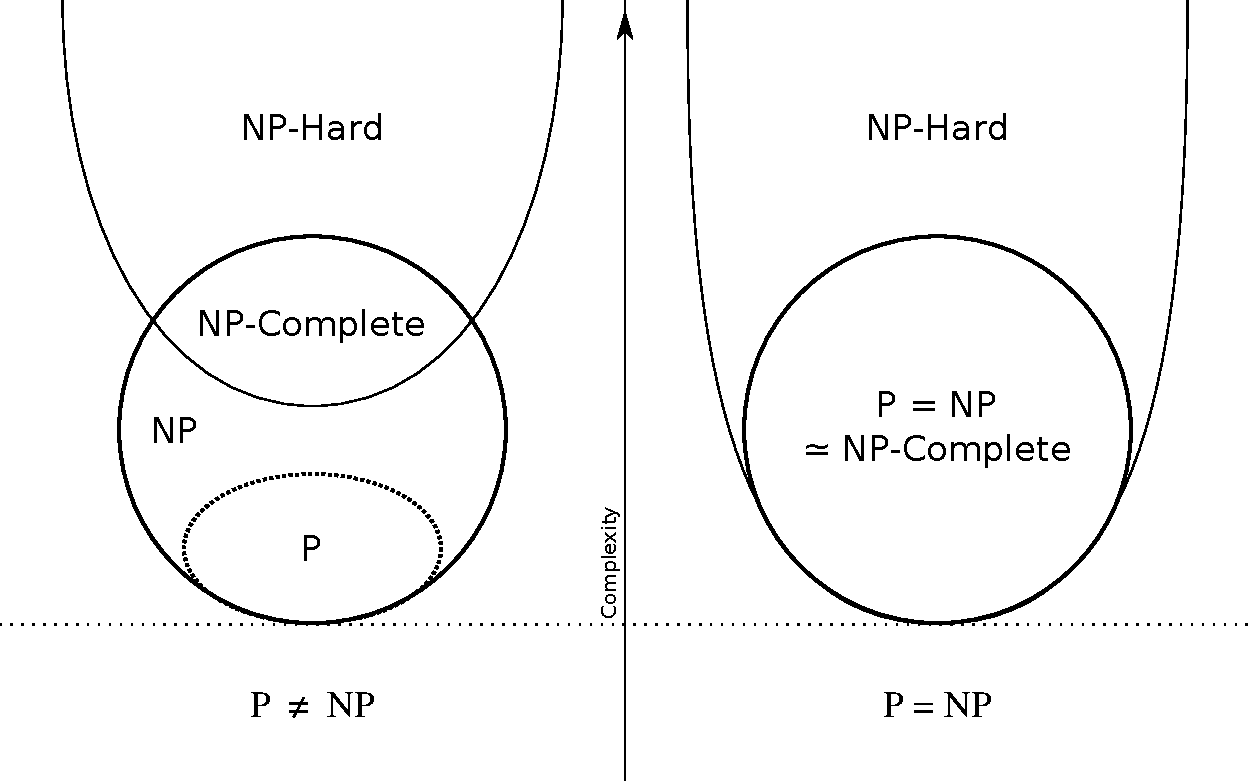
\includegraphics[scale=.4]{images/Euler-Diagram-P-NP-NPh-NPc.pdf}
	\caption{Ойлерова диаграма за класовете P, NP, NP-h и NP-c}
\end{figure}
\noindent
Изобщо не е тривиално да се докаже, че ВСИЧКИ задачи за разпознаване от NP са Karp\,-\,сводими до дадена задача за разпознаване. Ако имаме такава задача и при това намерим детерминирано полиномиално нейно решение, то ще имаме детерминирано полиномиално решение на ВСИЧКИ задачи за разпознаване от NP, откъдето ще следва, че P=NP. Първата задача за разпознаване, за която е доказано, че е NP-hard е така наречената SAT (от satisfiability):
\begin{boxzzr}{SAT}{sat}
	\dproblem{\varphi$ - булева формула в КНФ$}{$Удволетворима ли е $\varphi$?$}
\end{boxzzr}
\begin{examplecp}
	$\begin{cases}
		\varphi=(x_1\lor x_2\lor x_3\lor x_4)\land(\overline{x_1}\lor x_2\lor\overline{x_5}\lor x_8)\land(\overline{x_1}\lor\overline{x_2})\land x_6\land x_7\\\
		\!\!\text{да //сертификат: }\langle x_1,x_2,x_3,x_4,x_5,x_6,x_7,x_8\rangle=\langle T,F,F,T,F,T,T,F\rangle
	\end{cases}$
\end{examplecp}\leavevmode\newline

\begin{boxtheorem}{Cook-Levin}{}
	SAT е NP-трудна.
\end{boxtheorem}
\begin{proof}
	Накратко, само идеята. Всеки недетерминиран алгоритъм може да се представи чрез недетерминирана машина на тюринг (всъщност "истинската"\ дефиницията на NP използва недетерминирани МТ, вместо недетерминирани алгоритми). Тази машина бива представяна чрез булеви формули, т.е. състоянията ѝ, преходите ѝ, началните ѝ състояния, финалните ѝ състояния, лентата ѝ и т.н., като "връзките"\ между тях биват правени отново чрез булеви формули. Съответно тези формули са в КНФ.
\end{proof}\vspace{0.3cm}

\noindent
Следното твърдение ще ни е основния инструмент, с помощта на който ще доказваме, че дадена задача за разпознаване е NP-трудна. Съответно е инструмент, с който да доказваме, че не сме ние глупавите, а че самите задачи са с трудна природа (тоест никой човек досега не е успял да ги реши полиномиално).
\begin{boxproposition}{}{}
	Нека $\mathcal{A},\mathcal{B}\in\mathcal{DP}$. Тогава ако $\mathcal{B}\in$ NP-h и $\mathcal{B}\le_p\mathcal{A}$, то $\mathcal{A}\in$ NP-h.
\end{boxproposition}
\begin{proof}
	Нека $\mathcal{C}$ е произволна от NP. Тъй като $\mathcal{B}\in$ NP-h, то $\mathcal{C}\le_p\mathcal{B}$, но по условие имаме $\mathcal{B}\le_p\mathcal{A}$. Сега от транзитивността имаме $\mathcal{C}\le_p\mathcal{A}$. Но $\mathcal{C}\in$ NP беше произолно, следователно $\big(\forall\mathcal{C}\in$ NP$\big)\big(\mathcal{C}\le_p\mathcal{A}\big)$, т.е. $\mathcal{A}\in$ NP-h (по дефиниция).
\end{proof}

%	\begin{pseudocode}
%		\SetKwData{Left}{left}\SetKwData{This}{this}\SetKwData{Up}{up}
%		\SetKwFunction{Union}{Union}\SetKwFunction{FindCompress}{FindCompress}
%		\SetKwInOut{Input}{input}\SetKwInOut{Output}{output}
%		Function2(a,b)://a-int, b-float\\
%		%		\BlankLine
%		\Begin{
%			\emph{special treatment of the first line}\;
%			\For{$i\leftarrow 2$ \KwTo $l$}{
%				\emph{special treatment of the first element of line $i$}\;
%				\For{$j\leftarrow 2$ \KwTo $w$}{\label{forins}
%					\Left$\leftarrow$ \FindCompress{$Im[i,j-1]$}\;
%					\Up$\leftarrow$ \FindCompress{$Im[i-1,]$}\;
%					\This$\leftarrow$ \FindCompress{$Im[i,j]$}\;
%					\If(\tcp*[h]{O(\Left,\This)==1}){\Left compatible with \This}{\label{lt}
%						\lIf{\Left $<$ \This}{\Union{\Left,\This}}
%						\lElse{\Union{\This,\Left}}
%					}
%					\If(\tcp*[f]{O(\Up,\This)==1}){\Up compatible with \This}{\label{ut}
%						\lIf{\Up $<$ \This}{\Union{\Up,\This}}
%						\tcp{\This is put under \Up to keep tree as flat as possible}\label{cmt}
%						\lElse{\Union{\This,\Up}}%\tcp*[h]{\This linked to \Up}\label{lelse}
%					}
%				}
%				\lForEach{element $e$ of the line $i$}{\FindCompress{p}}
%			}
%		}
%		\caption{disjoint decomposition}\label{algo_disjdecomp}
%	\end{pseudocode}


\end{document}